% Paquets généraux
\documentclass[a4paper,12pt,titlepage,twoside]{article}
\usepackage[T1]{fontenc}
\usepackage[utf8]{inputenc}
\usepackage[french]{babel}
\usepackage{subcaption}
\addto\captionsfrench{%
  \renewcommand{\tablename}{Tableau}%
}
\usepackage[gen]{eurosym}
%\usepackage[dvips]{graphicx}
\usepackage{minted}
\usepackage{fancyhdr}
\usepackage{pdfpages} 
\usepackage{multido}
\usepackage{hyperref}
\usepackage{textcomp}
\usepackage{schemabloc}
%\usepackage[bitstream-charter]{mathdesign}
\usepackage{array}
\newcolumntype{P}[1]{>{\centering\arraybackslash}p{#1}}
\usepackage[shortlabels]{enumitem}
\usepackage[framemethod=TikZ]{mdframed}

\newcommand{\id}{71}
\newcommand{\nom}{Théorie des mécanismes}
\newcommand{\sequence}{04}
\newcommand{\nomsequence}{Liaisons entre les solides}
\newcommand{\num}{02}
\newcommand{\type}{KH}
\newcommand{\descrip}{Liaisons équivalentes, hyperstatisme, liaisons en série et en parallèle, théorie des graphes}
\newcommand{\competences}{B2-12: Proposer une modélisation des liaisons avec leurs caractéristiques géométriques. \\ &  B2-13: Proposer un modèle cinématique paramétré à partir d'un système réel, d'une maquette numérique ou d'u \\ &  B2-17: Simplifier un modèle de mécanisme. \\ &  B2-18: Modifier un modèle pour le rendre isostatique. \\ &  C1-04: Proposer une démarche permettant d'obtenir une loi entrée-sortie géométrique.  \\ &  C2-05: Caractériser le mouvement d'un repère par rapport à un autre repère. \\ &  C2-06: Déterminer les relations entre les grandeurs géométriques ou cinématiques. }
\newcommand{\nbcomp}{7}
\newcommand{\systemes}{}
\newcommand{\systemesnum}{}
\newcommand{\systemessansaccent}{}
\newcommand{\ilot}{2}
\newcommand{\ilotstr}{02}
\newcommand{\dossierilot}{\detokenize{Ilot_02 }}

%\usepackage{style}
\usepackage{bodegraph}
\usepackage{rpcinematik}
\usepackage[locale = FR]{siunitx}
\usepackage{caption}
\newcommand{\institute}{Lycée Dorian}

\usepackage{listings}
\usepackage{fancyvrb}
\usepackage{color}
\usepackage{xcolor}
\usepackage{colortbl}
\usepackage{helvet}
\usepackage[frenchmath]{newtxsf} % for sans serif symbols
\renewcommand{\familydefault}{\sfdefault}
%\usepackage{amsfonts}
%\usepackage{amsmath}
%\usepackage{lmodern}
\usepackage{mathastext}
%\usepackage{xspace}
\usepackage{varioref}
\usepackage{tabularx}
%\usepackage{floatflt}
\usepackage{graphics}
\usepackage{wrapfig}
\usepackage{textcomp}
\usepackage{tikz,tkz-tab}
\usepackage[european resistor, european voltage, european current]{circuitikz}
\usepackage{wrapfig}
\usepackage{gensymb}
\usepackage[percent]{overpic}
\usetikzlibrary{babel}
\usepackage{ifthen}
\usepackage{cancel}
\usepackage{etoolbox}
\usepackage{multirow}
%\usepackage{boxedminipage}
\definecolor{gris25}{gray}{0.75}
\definecolor{bleu}{RGB}{18,33,98}
\definecolor{bleuf}{RGB}{42,94,171}
\definecolor{bleuc}{RGB}{231,239,247}
\definecolor{bleum}{RGB}{160,195,226}
\definecolor{rougef}{RGB}{185,18,27}
\definecolor{rougec}{RGB}{255,188,204}%255,230,231
\definecolor{vertf}{RGB}{103,126,82}
\definecolor{vertc}{RGB}{220,255,191}
\definecolor{forestgreen}{rgb}{0.13,0.54,0.13}
\definecolor{blcr}{rgb}{0.59,0.69,0.84}
\definecolor{blfr}{rgb}{0.32,0.51,0.75}
\definecolor{orfr}{rgb}{0.90,0.42,0.15}
\definecolor{orcr}{rgb}{0.90,0.65,0.50}
\definecolor{orangef}{rgb}{0.659,0.269,0.072}
\definecolor{orange}{rgb}{0.58,0.35,0.063}
\definecolor{orangec}{rgb}{0.43,0.32,0.25}
\definecolor{rcorrect}{rgb}{0.6,0,0}
\definecolor{sequence}{rgb}{0.75,0.75,0.75}
\definecolor{competences}{rgb}{0.61,0.73,0.35}
\definecolor{rose}{HTML}{ff00ff}
\definecolor{grisf}{HTML}{222222}
\definecolor{grisc}{HTML}{636363}
\definecolor{normal}{HTML}{4087c4}
\definecolor{info}{HTML}{5bc0de}
\definecolor{success}{RGB}{92,184,92}
\definecolor{warning}{RGB}{240,173,78}
\definecolor{danger}{RGB}{217,83,79}
\hypersetup{                    % parametrage des hyperliens
    colorlinks=true,                % colorise les liens
    breaklinks=true,                % permet les retours à la ligne pour les liens trop longs
    urlcolor= blfr,                 % couleur des hyperliens
    linkcolor= orange,                % couleur des liens internes aux documents (index, figures, tableaux, equations,...)
    citecolor= forestgreen                % couleur des liens vers les references bibliographiques
    }

\newcolumntype{M}[1]{>{\centering\arraybackslash}m{#1}}
\definecolor{codegreen}{rgb}{0,0.6,0}
\definecolor{codegray}{rgb}{0.5,0.5,0.5}
\definecolor{codepurple}{rgb}{0.58,0,0.82}
\definecolor{backcolour}{rgb}{0.95,0.95,0.92}

\lstdefinestyle{mystyle}{
    backgroundcolor=\color{backcolour},   
    commentstyle=\color{codegreen},
    keywordstyle=\color{magenta},
    numberstyle=\tiny\color{codegray},
    stringstyle=\color{codepurple},
    basicstyle=\ttfamily\footnotesize,
    breakatwhitespace=false,         
    breaklines=true,                 
    captionpos=b,                    
    keepspaces=true,                 
    numbers=left,                    
    numbersep=5pt,                  
    showspaces=false,                
    showstringspaces=false,
    showtabs=false,                  
    tabsize=2
}

\lstset{style=mystyle}

% Mise en page
\pagestyle{fancy}

\setlength{\hoffset}{-18pt}
\setlength{\oddsidemargin}{0pt} 	% Marge gauche sur pages impaire2s
\setlength{\evensidemargin}{0pt} 	% Marge gauche sur pages paires
\setlength{\marginparwidth}{00pt} 	% Largeur de note dans la marge
\setlength{\headwidth}{481pt} 	 	% Largeur de la zone de tête (17cm)
\setlength{\textwidth}{481pt} 	 	% Largeu\textbf{r de la zone de texte (17cm)
\setlength{\voffset}{-18pt} 		% Bon pour DOS
\setlength{\marginparsep}{7pt}	 	% Séparation de la marge
\setlength{\topmargin}{-30pt} 		% Pas de marge en haut
\setlength{\headheight}{55pt} 		% Haut de page
\setlength{\headsep}{20pt} 		% Entre le haut de page et le texte
\setlength{\footskip}{30pt} 		% Bas de\textbf{ page + séparation
\setlength{\textheight}{700pt} 		% Hauteur de l'icone zone de texte (25cm)
\setlength\fboxrule{1 pt}
\renewcommand{\baselinestretch}{1}
\setcounter{tocdepth}{1}
\newcommand{\cadre}[2]
{\fbox{
  \begin{minipage}{#1\linewidth}
   \begin{center}
    #2\\
   \end{center}
  \end{minipage}
 }
}

\newcommand{\repon}[1]
{
~\ \\
\begin{tabular}{|m{\linewidth}|}
 \hline
\multido{}{#1}{\\ \hline}
\end{tabular}
}


\newcommand{\objectif}[1]{
\mdfsetup{%
frametitle={%
\tikz[baseline=(current bounding box.east),outer sep=0pt]
\node[anchor=east,rectangle,fill=bleum]
{\strut Objectif~};}}
\mdfsetup{innertopmargin=10pt,linecolor=bleum,%
linewidth=2pt,topline=true,%
frametitleaboveskip=\dimexpr-\ht\strutbox\relax
}
\begin{mdframed}[]\relax%
#1
\end{mdframed}}


\newcounter{num_quest} \setcounter{num_quest}{0}
\newcounter{num_rep} \setcounter{num_rep}{0}
\newcounter{num_cor} \setcounter{num_cor}{0}

\newcommand{\feuilleDR}[1]{
	\begin{tikzpicture}
		\draw[gray!30](0,0)grid[step=0.5cm](\linewidth,#1);
	\end{tikzpicture}
}

%\newcommand{\question}[1]{\refstepcounter{num_quest}\par
%~\ \\ \parbox[t][][t]{0.15\linewidth}{\textbf{Question \arabic{num_quest}}}\parbox[t][][t]{0.85\linewidth}{#1\label{q\the\value{num_quest}}}\par
%}

\newcommand{\question}[1]{\refstepcounter{num_quest}\par
~\ \\ \textbf{Question \arabic{num_quest} : }#1\label{q\the\value{num_quest}}\par
}

\newcommand{\posetafigure}[3]{
\begin{figure}[ht!]
 \begin{center}
  \includegraphics[width=#2\linewidth]{img/#1}
 \end{center}
 \caption{\label{#1} #3}
\end{figure}}

\newcommand{\goforum}{
\begin{figure}

\end{figure}
\begin{center}
 
\includegraphics[width=0.7\linewidth]{../../../img/go_forum}
\end{center}
\label{go_forum}
\caption{J'pète les plombs}
\end{figure}}

\newcommand{\reponse}[4][1]
{\noindent
\parbox{\textwidth}{
\rule{\linewidth}{.5pt}\\
\textbf{Question\ifthenelse{#1>1}{s}{} \multido{}{#1}{%
\refstepcounter{num_rep}\ref{q\the\value{num_rep}} }:} ~\ \\
\ifdef{\public}{#3 \ifthenelse{#2>0}{~\ \\ 	\feuilleDR{#2}}}{#4}
}}

\newcommand{\cor}
{\refstepcounter{num_cor}
\noindent
\rule{\linewidth}{.5pt}
\textbf{Question \arabic{num_cor}:} \\
}

\newcommand{\finsujet}
{
    \begin{center}
    \Large{FIN}
    \end{center}

    \cleardoublepage

    \ifdef{\public}{\pagestyle{docreponse}}{\pagestyle{correction}}

    \ifdef{\public}{
        \begin{tikzpicture} 
            \draw (0,0) rectangle (2,2);
            \draw (0,0) -- (2,2);
            \draw (1.5,0.5) node {\large 20};
            \draw (2.5,0) rectangle (16,2);
            \draw (4.5,1.7) node {\large Commentaires:};
        \end{tikzpicture}
    }
    ~\ \\
}


%\newcommand{\repcarre}[2]
%{
%~\ \\
%\begin{tikzpicture}
%\draw [fill=white] (0,0) rectangle +(\linewidth,#1);
%\node[align=left] at (1.1,#2-0.3) {\textbf{Question #1:}};
%\end{tikzpicture}
%}

\newcommand{\titre}[1]
{\begin{center}
\cadre{0.8}{\huge #1} 
\end{center}
}


%Définition des torseurs :
\newcommand{\torseur}[2]{\left\{\mathcal{#1}_{#2} \right\}}
\newcommand{\torseurh}[3]{\left\{\genfrac{}{}{0pt}{0}{#1}{#2}\right\}_{#3}}
\newcommand{\torseurv}[8]{\left\{
\begin{matrix}
#1 & #4 \\ #2 & #5 \\ #3 &#6
\end{matrix}
\right\}_{{#7},{#8}}}

%Définition des torseurs :
%\newcommand{\torseur}[2]{\left \{\mbox{\relsize{2}{$\mathcal {#1}$}\relsize{-2}}\phantom{}_{\mbox{\scriptsize $#2$}} \right \}}
%\newcommand{\torseurh}[3]{\left\{\genfrac{}{}{0pt}{0}{#1}{#2}\right\}_{#3}}
%\newcommand{\torseurv}[8]{
%\left\{\begin{array}{@{}c|c@{}} #1 & #4 \\ #2 & #5 \\ #3 & #6 \end{array} \right\}_{#7,#8}
%}
\newcommand{\derivee}[2]{\left.\dfrac{\d #1}{\d t}\right|_{#2}}
\newcommand{\tripleint}{\int\!\!\!\!\!\int\!\!\!\!\!\int}

% Notation cinématique et statique
\newcommand{\cinematique}[2]{\mbox{#1}/\mbox{#2}}
\newcommand{\statique}[2]{\mbox{#1}\rightarrow\mbox{#2}}
\newcommand{\moment}[3]{\vv {#1}_{\scriptsize{#3}}(#2)}
\newcommand{\resultante}[2]{\vv {#1}_{\scriptsize{#2}}}


%Commande de base
\newcommand{\jo}{\left(j\omega\right)} % j \omega dans l'analyse fréquentielle
\newcommand{\tl}{\xrightarrow{\mathcal{L}}} % transformée de laplace sur fleche
\newcommand{\tli}{\xrightarrow{\mathcal{L}^{-1}}} % transformée inverse de laplace sur fleche
\renewcommand{\d}[1][]{\mathrm{d#1}}
\newcommand{\dd}[1][]{\mathrm{d#1}}
\newcommand{\vect}[2]{{#1}\wedge{#2}}
\newcommand{\base}[3]{(\vec #1,\vec #2,\vec #3)}
\newcommand{\vectbase}[4]{{\vphantom{\left| \begin{matrix}
#1\\#2\\#3 \end{matrix} \right|}}_{#4}{\left| \begin{matrix}
#1\\#2\\#3 \end{matrix} \right.}}
%Pour avoir les paragraphes sous la forme I, II, III
\renewcommand{\thesection}{\Roman{section}}
\setcounter{secnumdepth}{3}
\renewcommand{\Frlabelitemii}{$\bullet$}

% En tête et pied de page
\lhead{\nom}
\rhead{
\includegraphics[width=2cm]{../../../img/logo}}
\lfoot{\auteurun,\ \auteurdeux}
\cfoot{Page \thepage}

\fancypagestyle{docreponse}{%
  \fancyhf{}
  \fancyhead[LO]{NOM Prénom: .............................}
  \rhead{
\includegraphics[width=2cm]{../../../img/logo}\hspace{2pt}}
  \ifdef{\auteurdeux}{\lfoot{\auteurun,\ \auteurdeux}}{\lfoot{\auteurun}}
  \rfoot{\nom}
  \lfoot{Document réponse}
  \cfoot{Page \thepage}
   }

\fancypagestyle{correction}{%
  \fancyhf{}
  \lhead{\colorbox{danger}{\begin{minipage}{0.65\paperwidth} \textcolor{white}{\textbf{Correction}} \end{minipage}} }
  \rhead{
\includegraphics[width=2cm]{../../../img/logo}}
  \lfoot{Renaud Costadoat, Françoise Puig}
  \rfoot{\colorbox{danger}{\begin{minipage}{0.4\paperwidth} \begin{flushright}\textcolor{white}{\textbf{Correction}}\end{flushright} \end{minipage}} }}

\fancypagestyle{correctioninfo}{%
  \fancyhf{}
  \lhead{\colorbox{danger}{\begin{minipage}{0.65\paperwidth} \textcolor{white}{\textbf{Correction}} \end{minipage}} }
  \rhead{
\includegraphics[width=2cm]{../../../img/logo}}
  \lfoot{Renaud Costadoat, Juliette Genzmer}
  \rfoot{\colorbox{danger}{\begin{minipage}{0.6\paperwidth} \begin{flushright}\textcolor{white}{\textbf{Correction}}\end{flushright} \end{minipage}} }}

\renewcommand{\footrulewidth}{0.4pt}

\usepackage{eso-pic}
\newcommand{\BackgroundPic}{%
\put(0,0){%
\parbox[b][\paperheight]{\paperwidth}{%
\vfill
\begin{center}
\hspace{0.5cm}\vspace{0.5cm}

\includegraphics[width=\paperwidth,height=\paperheight,%
keepaspectratio]{../../../img/fond3}%
\end{center}
\vfill
}}}

\newcommand{\BackgroundPicdeux}{%
\put(25,-30){%
\parbox[b][\paperheight]{\paperwidth}{%
\vfill
\begin{center}
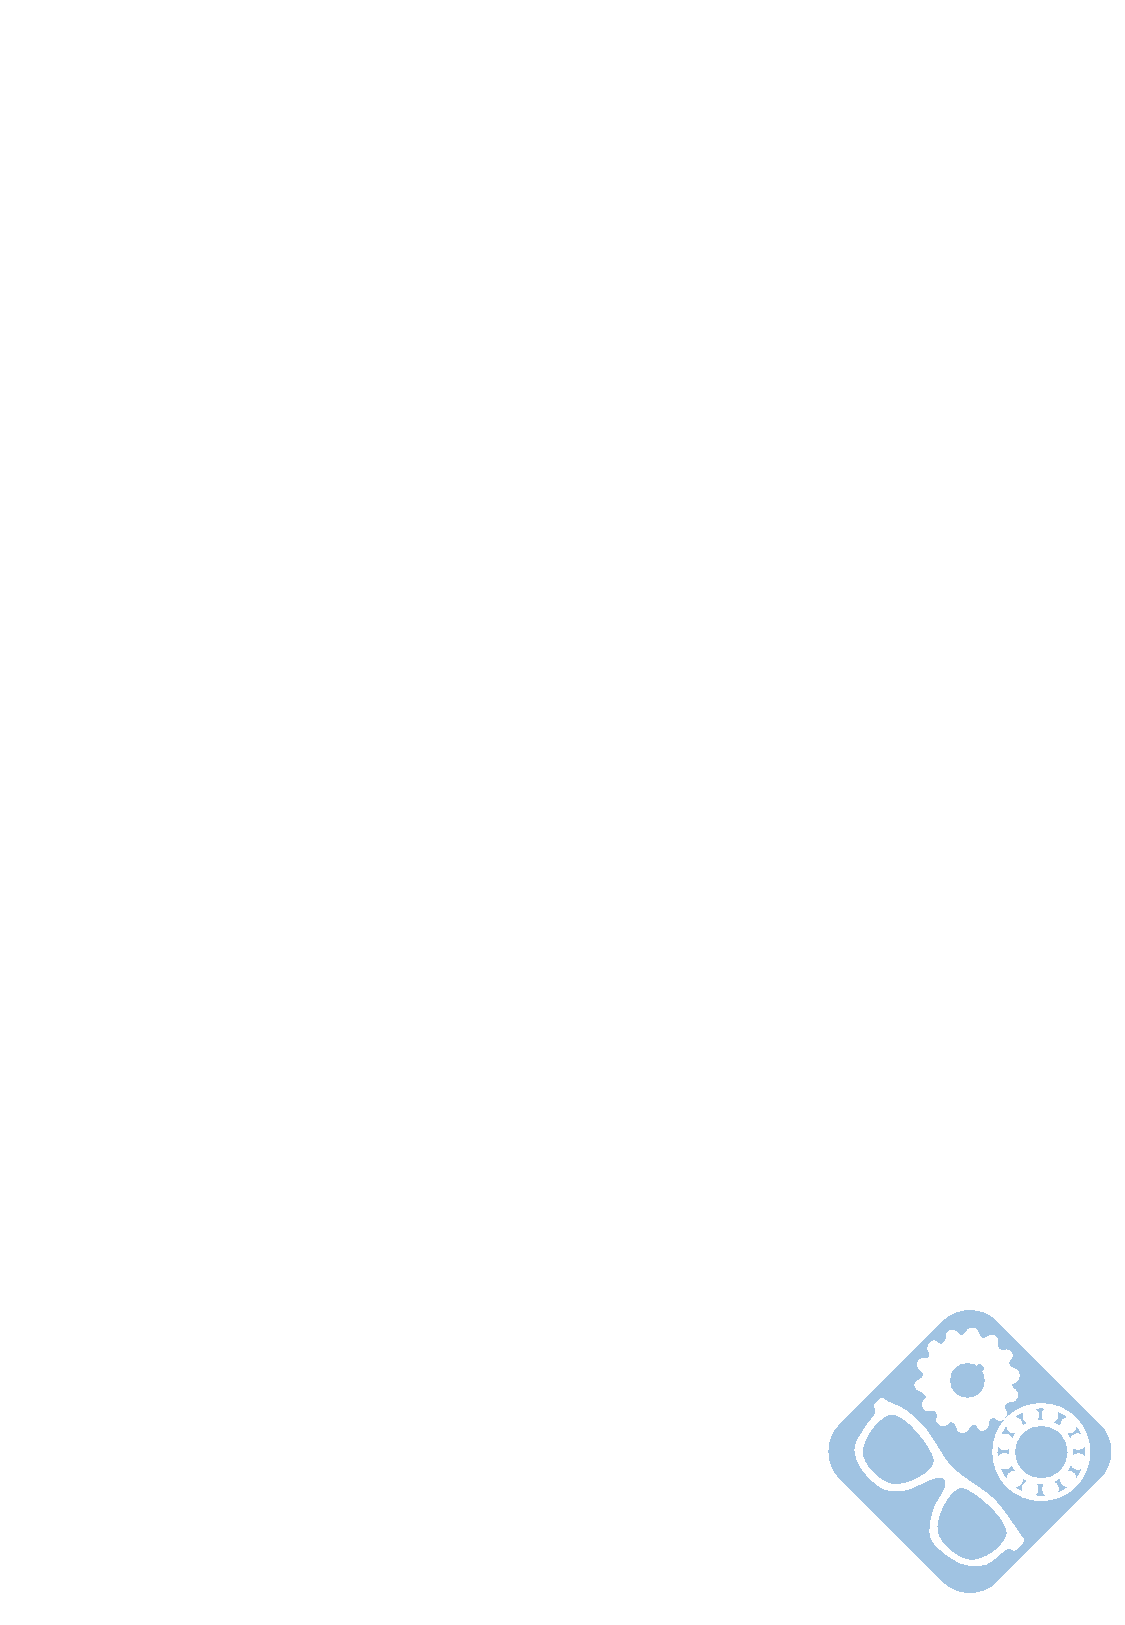
\includegraphics[width=\paperwidth,height=\paperheight,%
keepaspectratio]{../../../img/fond4}%
\end{center}
\vfill
}}}

\begin{document}

\pagestyle{empty}

\AddToShipoutPicture*{\BackgroundPic}


\includegraphics[width=2cm]{../../../img/logo}

\Huge{DS \numero - \sujet}

\vspace{1cm}

\ifdef{\prive}{\begin{center}\colorbox{danger}{\Huge{Avec Correction}}\end{center}}{}

\begin{center}
\centering\huge{PTSI}
\end{center}

\vspace{2cm}


\begin{center}
\centering\Large{\jour}
\end{center}

\vspace{2cm}

\normalsize

\tableofcontents

\newpage

\AddToShipoutPicture{\BackgroundPicdeux}

\pagestyle{fancy}

\begin{center}
\Huge \sujet
\end{center}


\normalsize



\paragraph{Présentation générale}

Le sujet porte sur l’étude d’une cabine de soudage (annexe 1 et figure \ref{img01}) qui permet l’assemblage d’une partie de l’armature d’assise de sièges automobiles.

\begin{figure}[!h]
\centering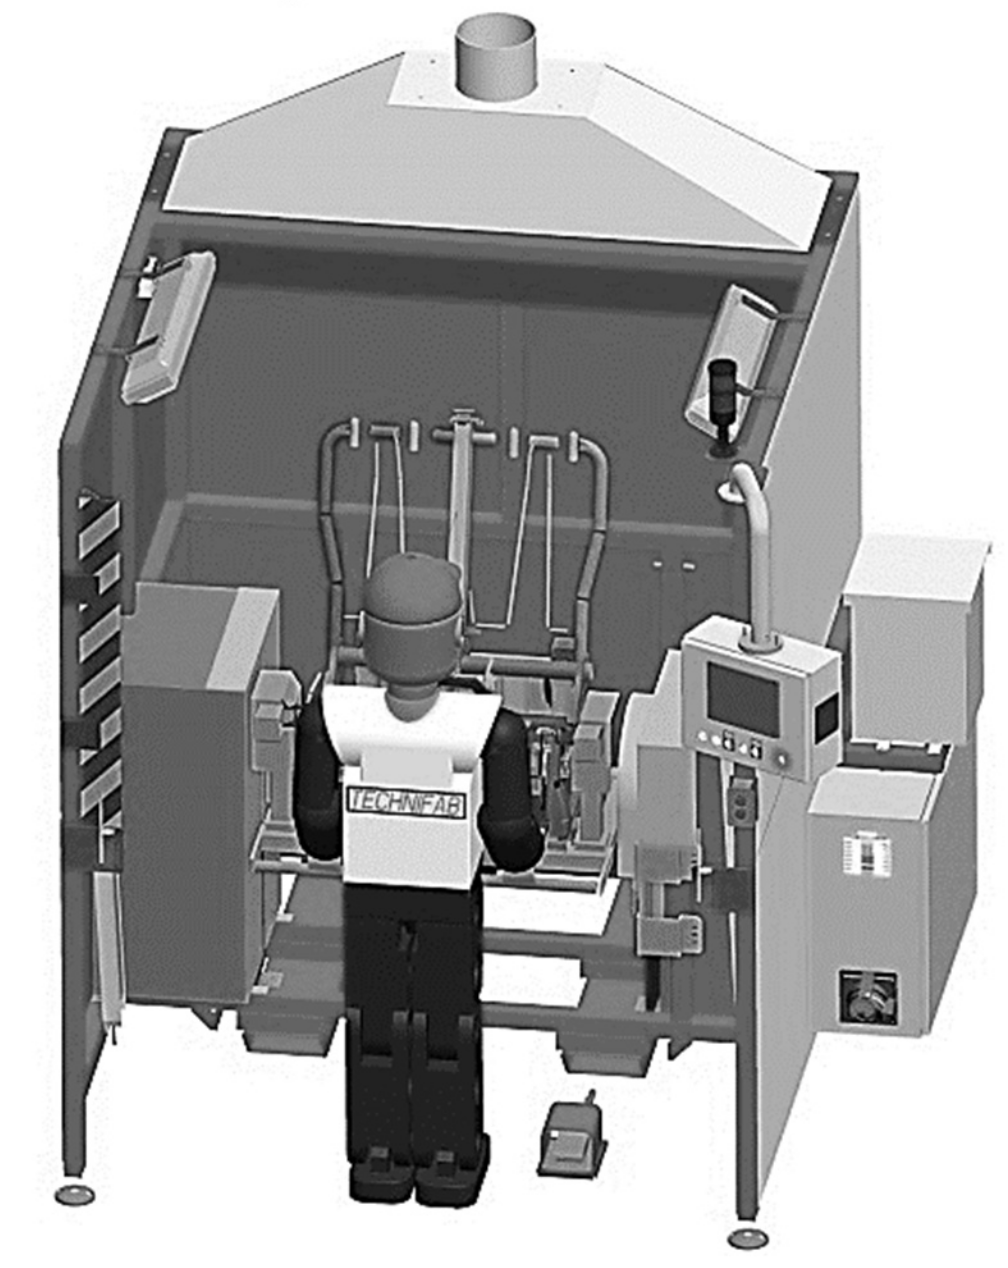
\includegraphics[width=0.35\linewidth]{img/fig01}
 \caption{Cabine de soudage}
 \label{img01}
\end{figure}

Le siège d’une automobile est composé d’une armature d’assise et d’un dossier, d’une mousse et d’une coiffe (figure \ref{img02}).

\begin{figure}[!h]
\centering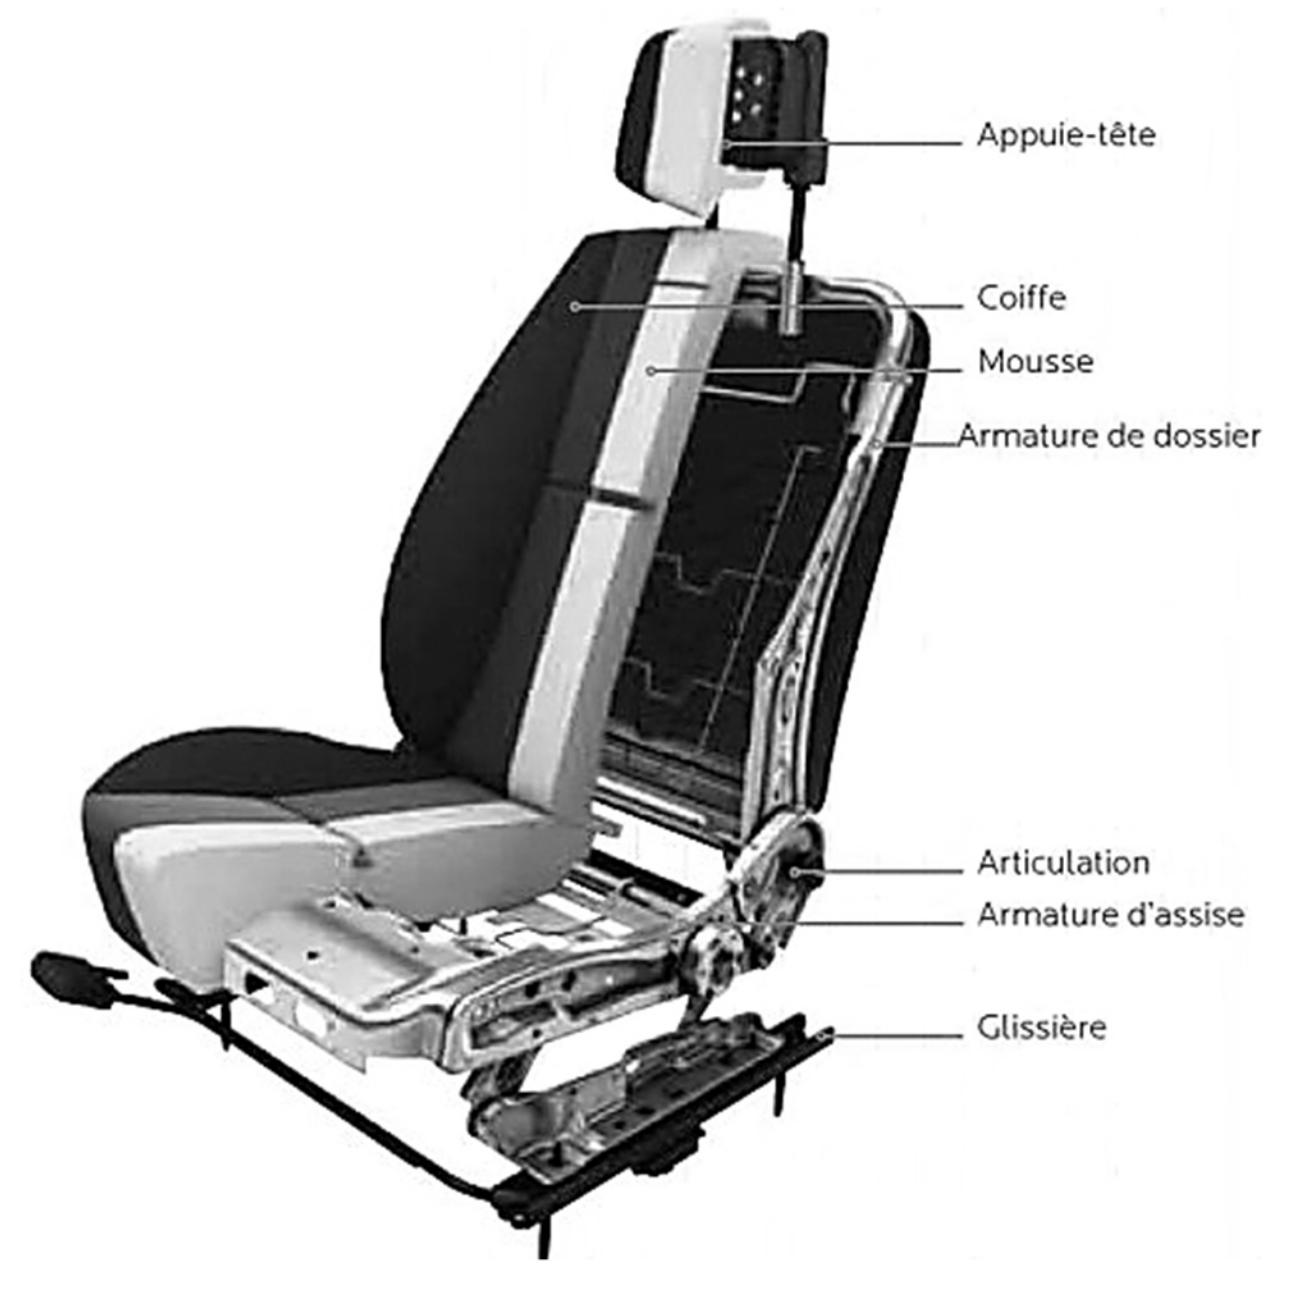
\includegraphics[width=0.5\linewidth]{img/fig02}
 \caption{Composition d’un siège automobile}
 \label{img02}
\end{figure}

La cabine de soudage permet la mise en place et le soudage de 4 fils sur l’armature d’une banquette arrière de véhicule de tourisme lors de sa fabrication (figure \ref{img03}). Dans le cas d’une banquette arrière, l’armature d’assise et l’armature de dossier ne font qu’une.

\begin{figure}[!h]
\centering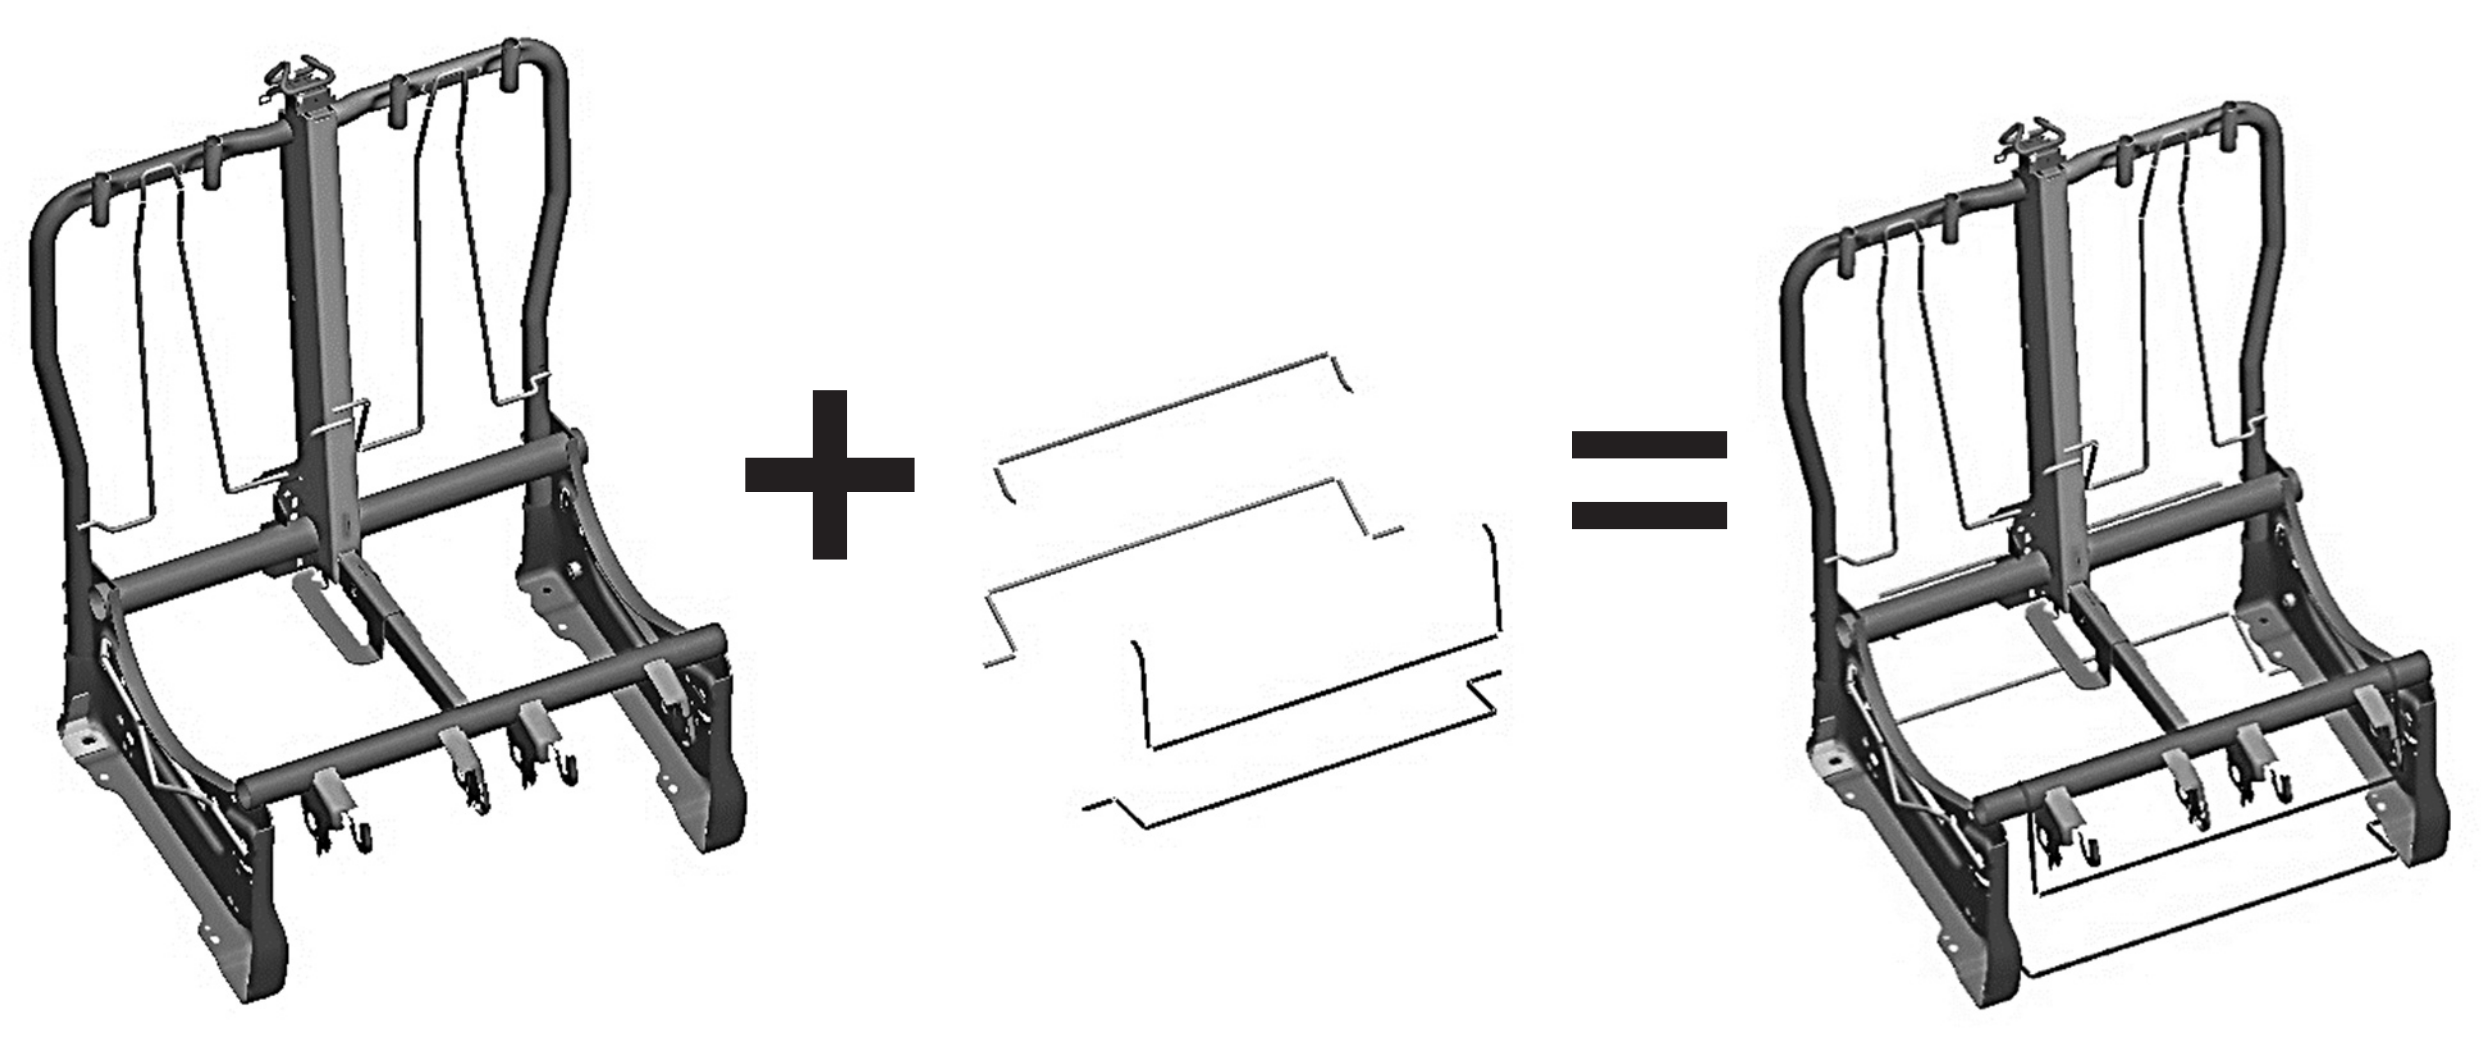
\includegraphics[width=0.8\linewidth]{img/fig03}
 \caption{Armature et fils à assembler}
 \label{img03}
\end{figure}

La cabine de soudage permet d’assurer une ergonomie optimale du poste de travail en s’adaptant à la taille de l’opérateur et en l’assistant dans les taches de bridage et de retournement de l’ensemble armature et fils (figure \ref{img04}).

\begin{figure}[!h]
\centering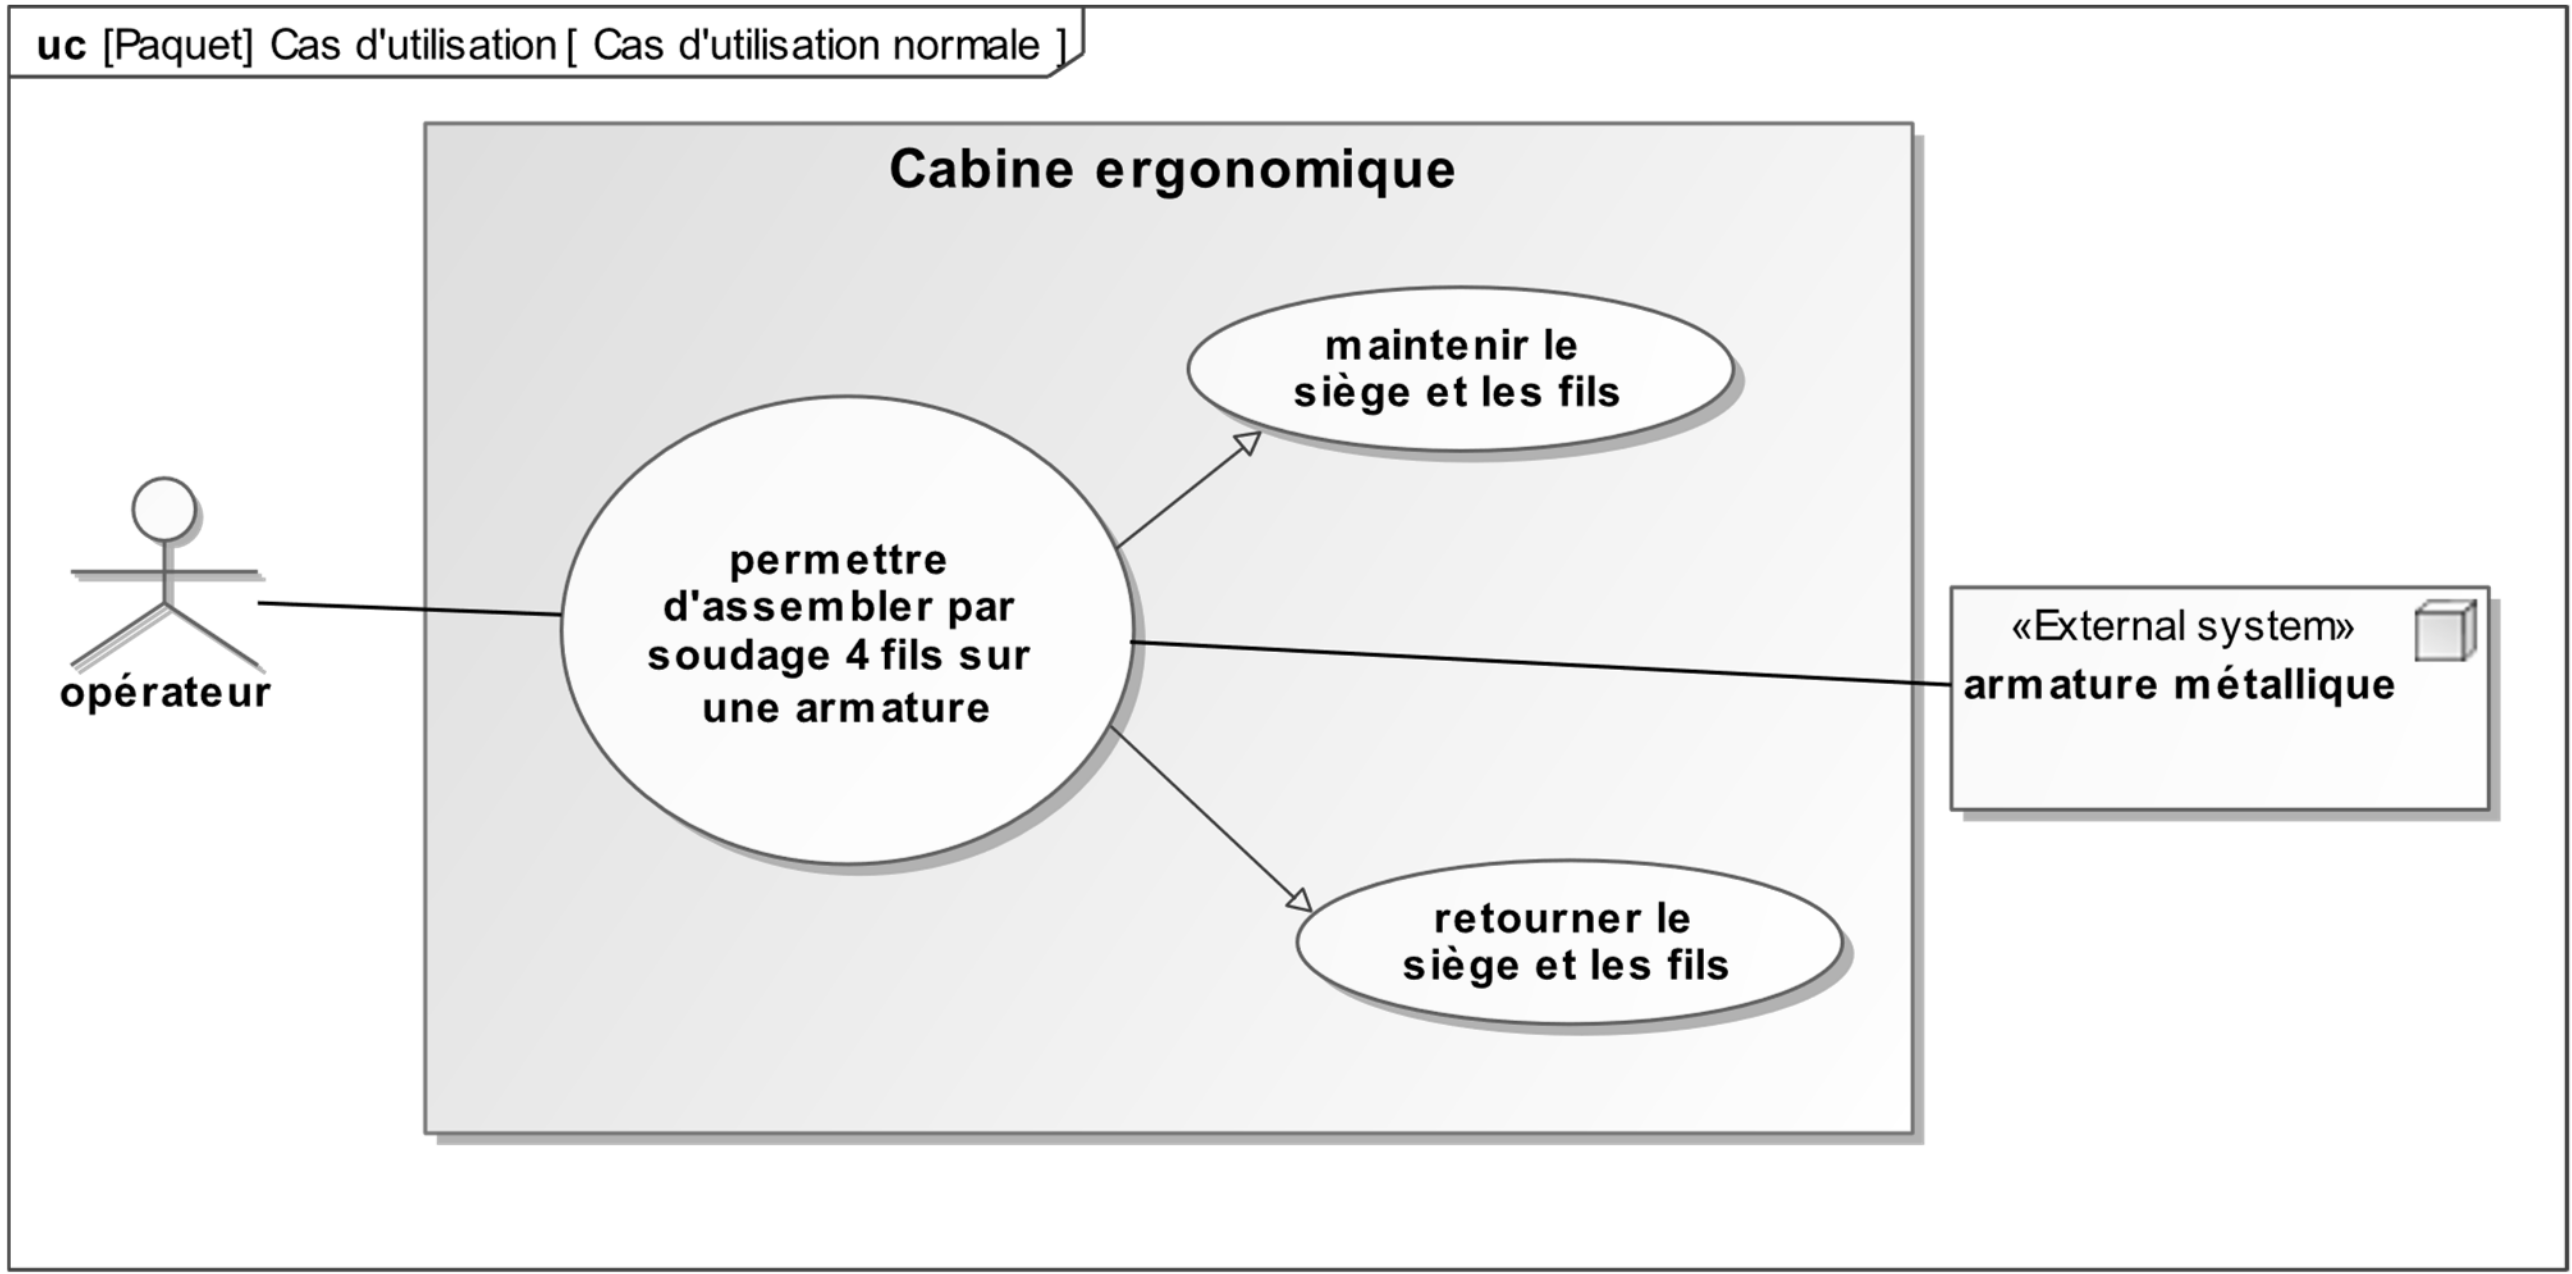
\includegraphics[width=\linewidth]{img/fig04}
 \caption{Diagramme des cas d’utilisation}
 \label{img04}
\end{figure}

En fin de processus de soudage, l’armature du siège est prête à être habillée.

Le cahier des charges partiel est donné et présente les acteurs en relation avec le système (figure \ref{img05}) ainsi que certaines exigences fonctionnelles (figure \ref{img06}) étudiées dans cette étude.

\begin{figure}[!h]
\centering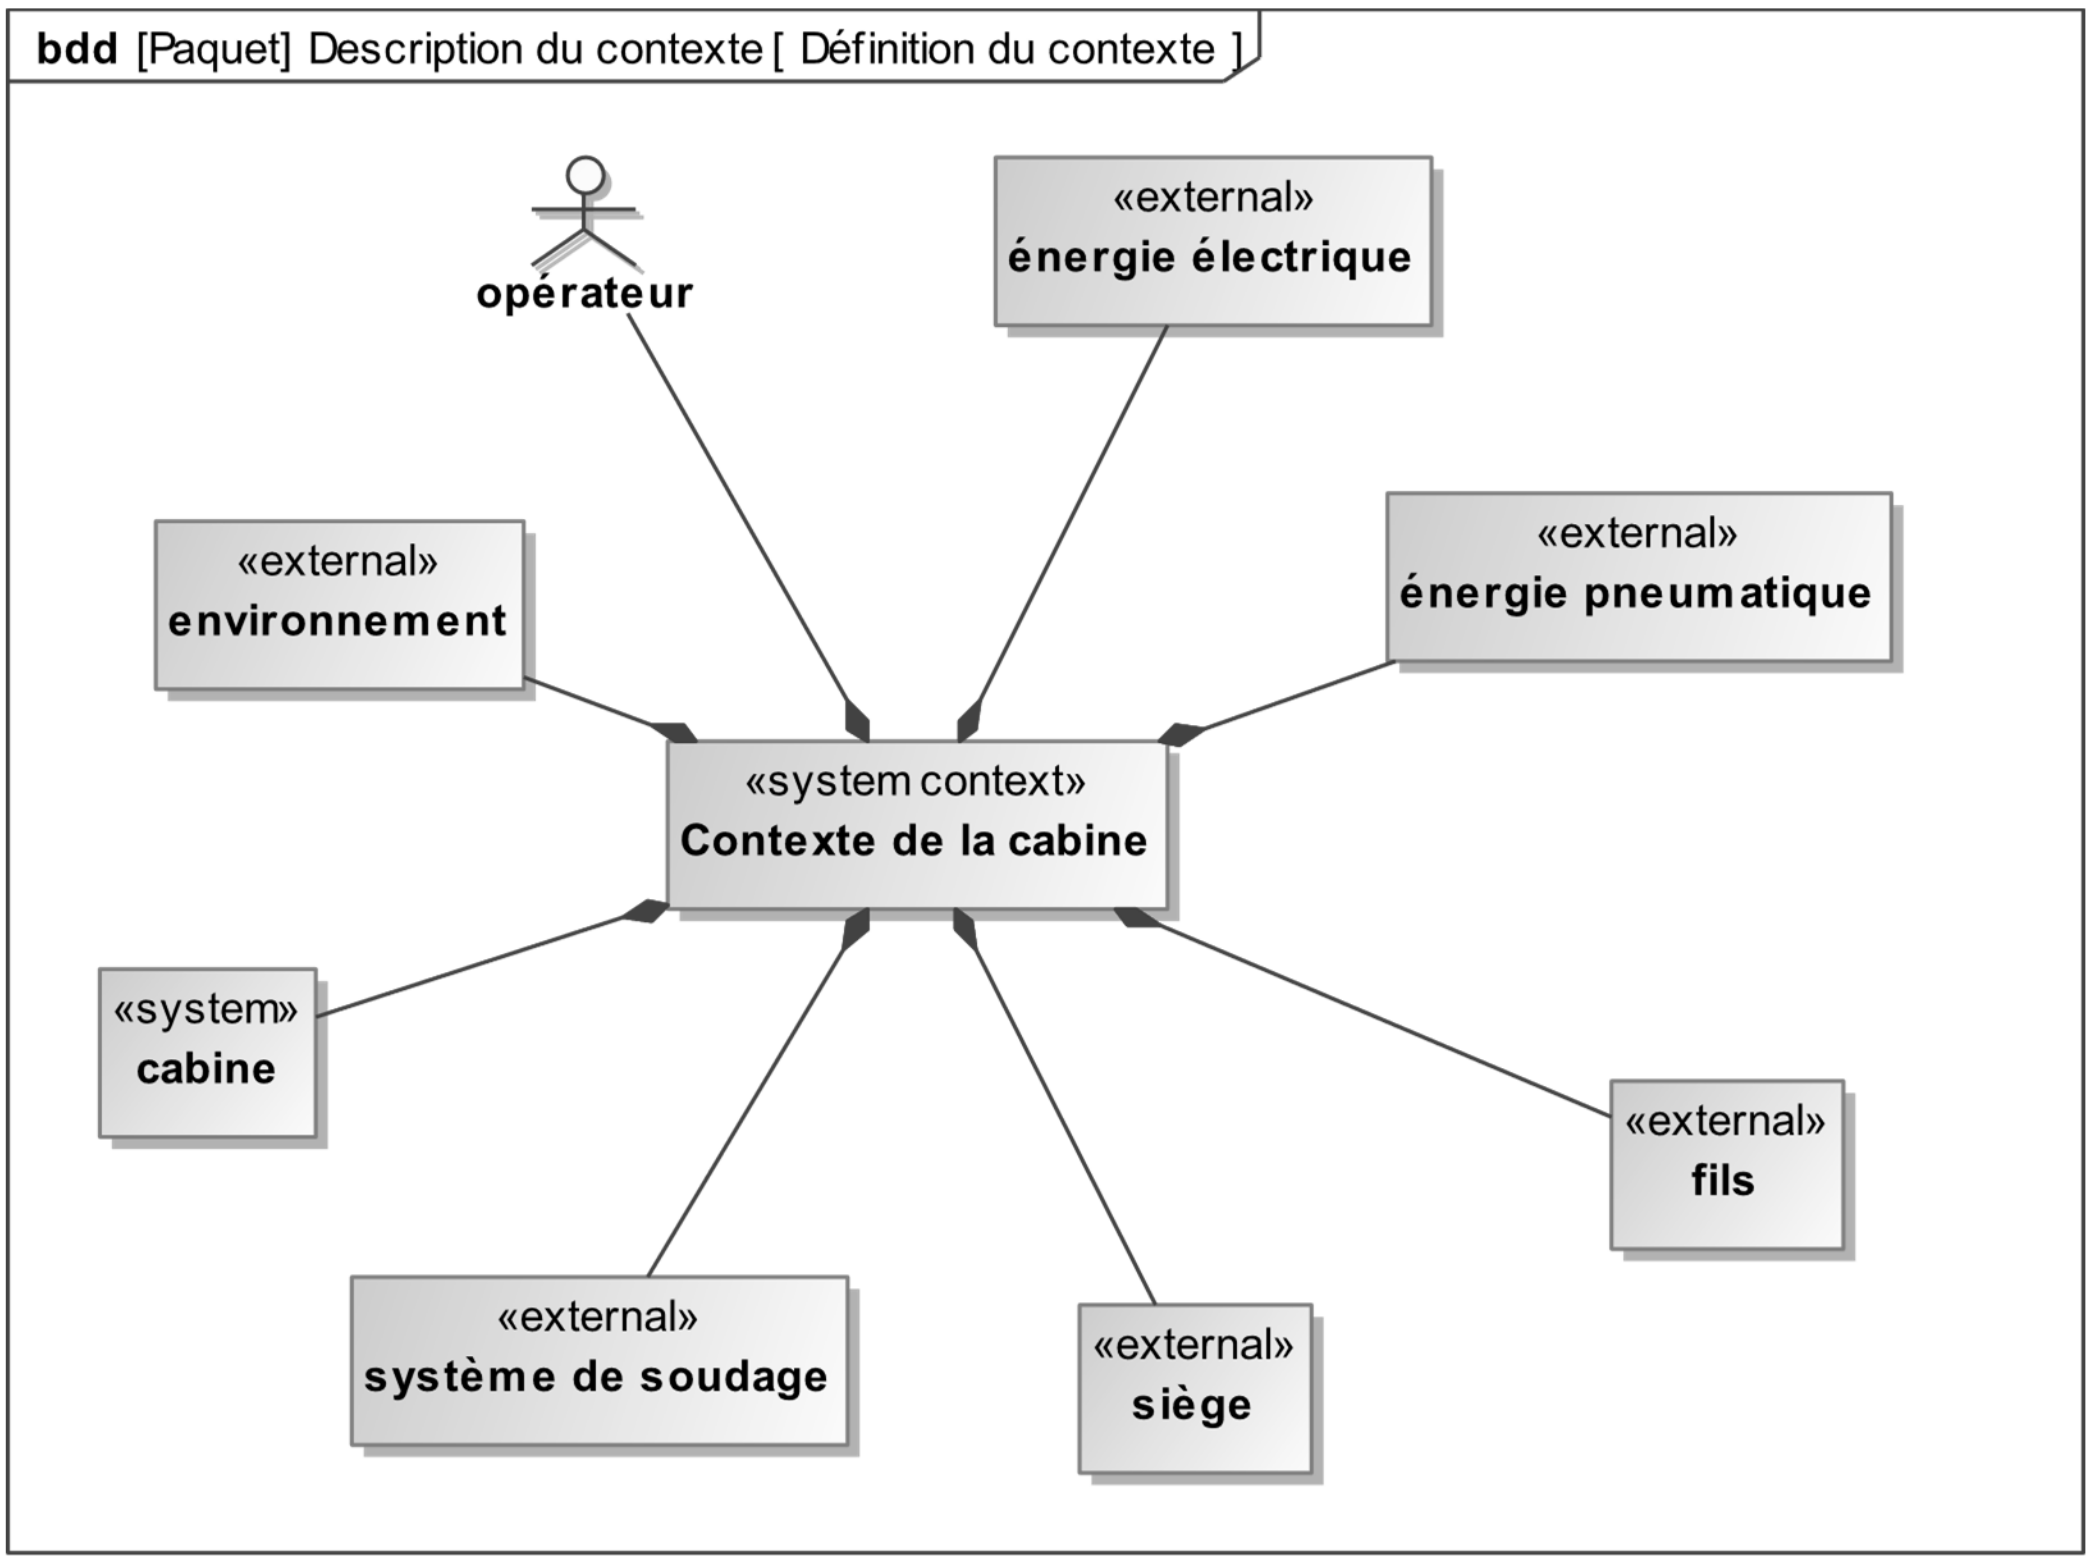
\includegraphics[width=\linewidth]{img/fig05}
 \caption{Définition du contexte}
 \label{img05}
\end{figure}

\begin{figure}[!h]
\centering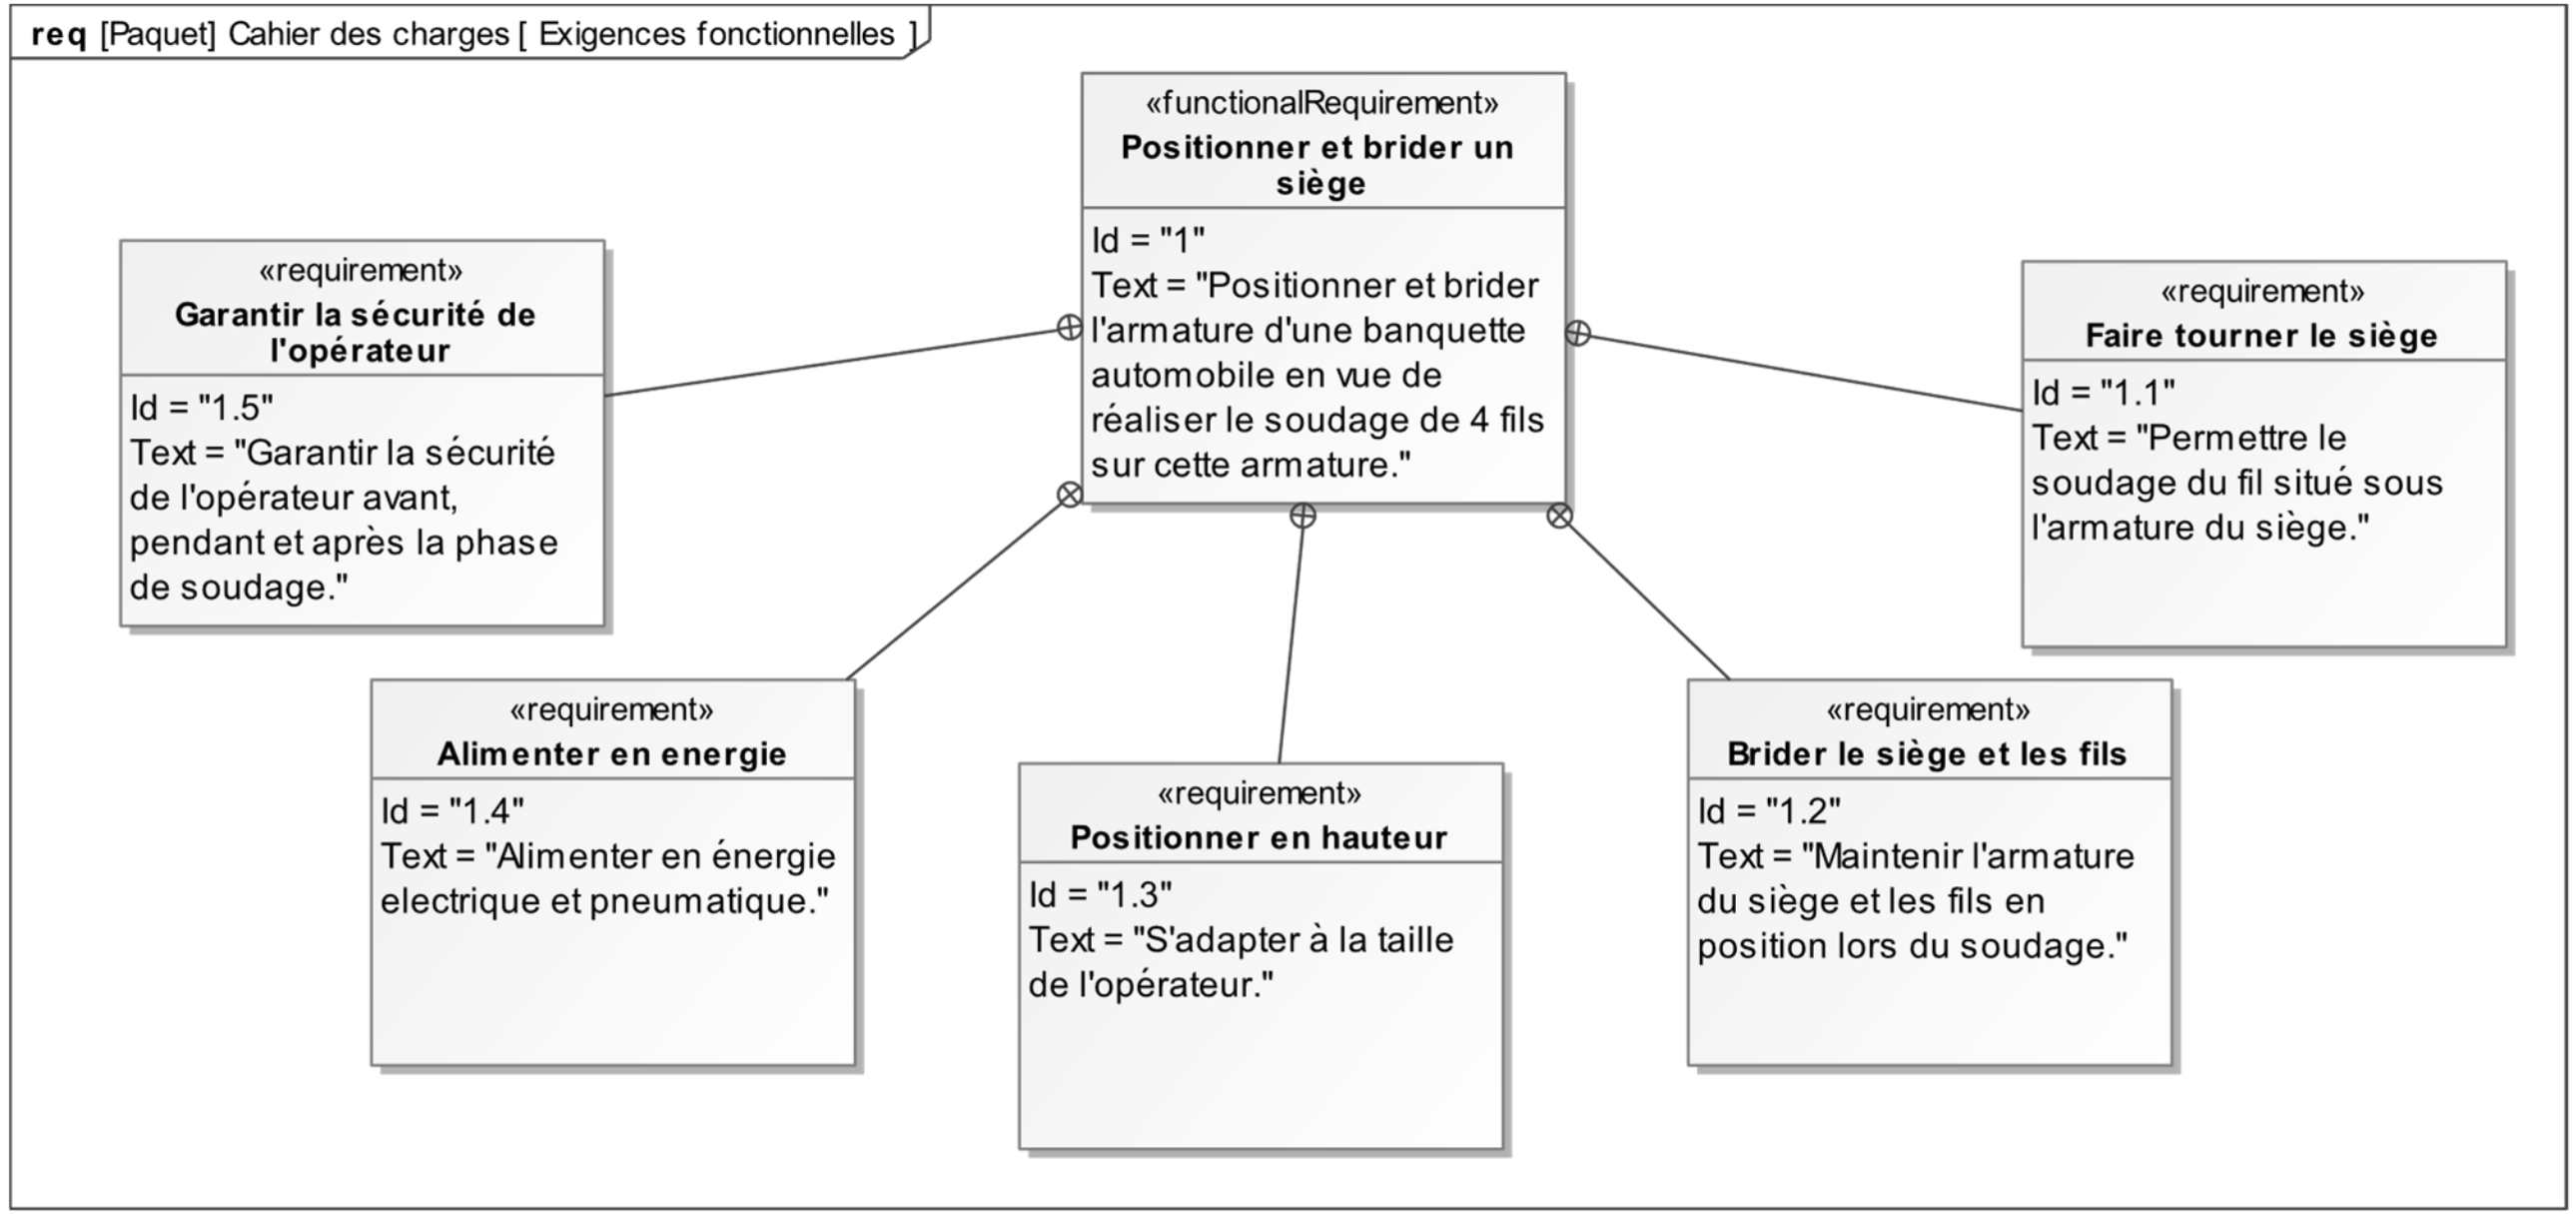
\includegraphics[width=\linewidth]{img/fig06}
 \caption{Exigences fonctionnelles}
 \label{img06}
\end{figure}

\clearpage

\section{Exigence \og Faire tourner le siège \fg}

Afin de faciliter la tâche de soudage à l’opérateur, il est possible de basculer l’ensemble du berceau dans deux positions de travail, permettant de souder par le dessus ou par le dessous.

Afin de s’adapter à la taille de l’opérateur, le système peut être réglé en hauteur. Ce réglage ne peut s’effectuer que si le berceau est en position horizontale. Un système d’indexage est présent dans la partie gauche de la machine. Cette position est captée par un détecteur de position tout ou rien actionné par une came placée sur l’axe de rotation (figure \ref{img07}).

\subsection{Étude de l’indexage de l’axe de rotation}

L’objectif de cette sous-partie est de concevoir la liaison encastrement de la came avec l’axe de rotation.

\begin{figure}[!h]
\centering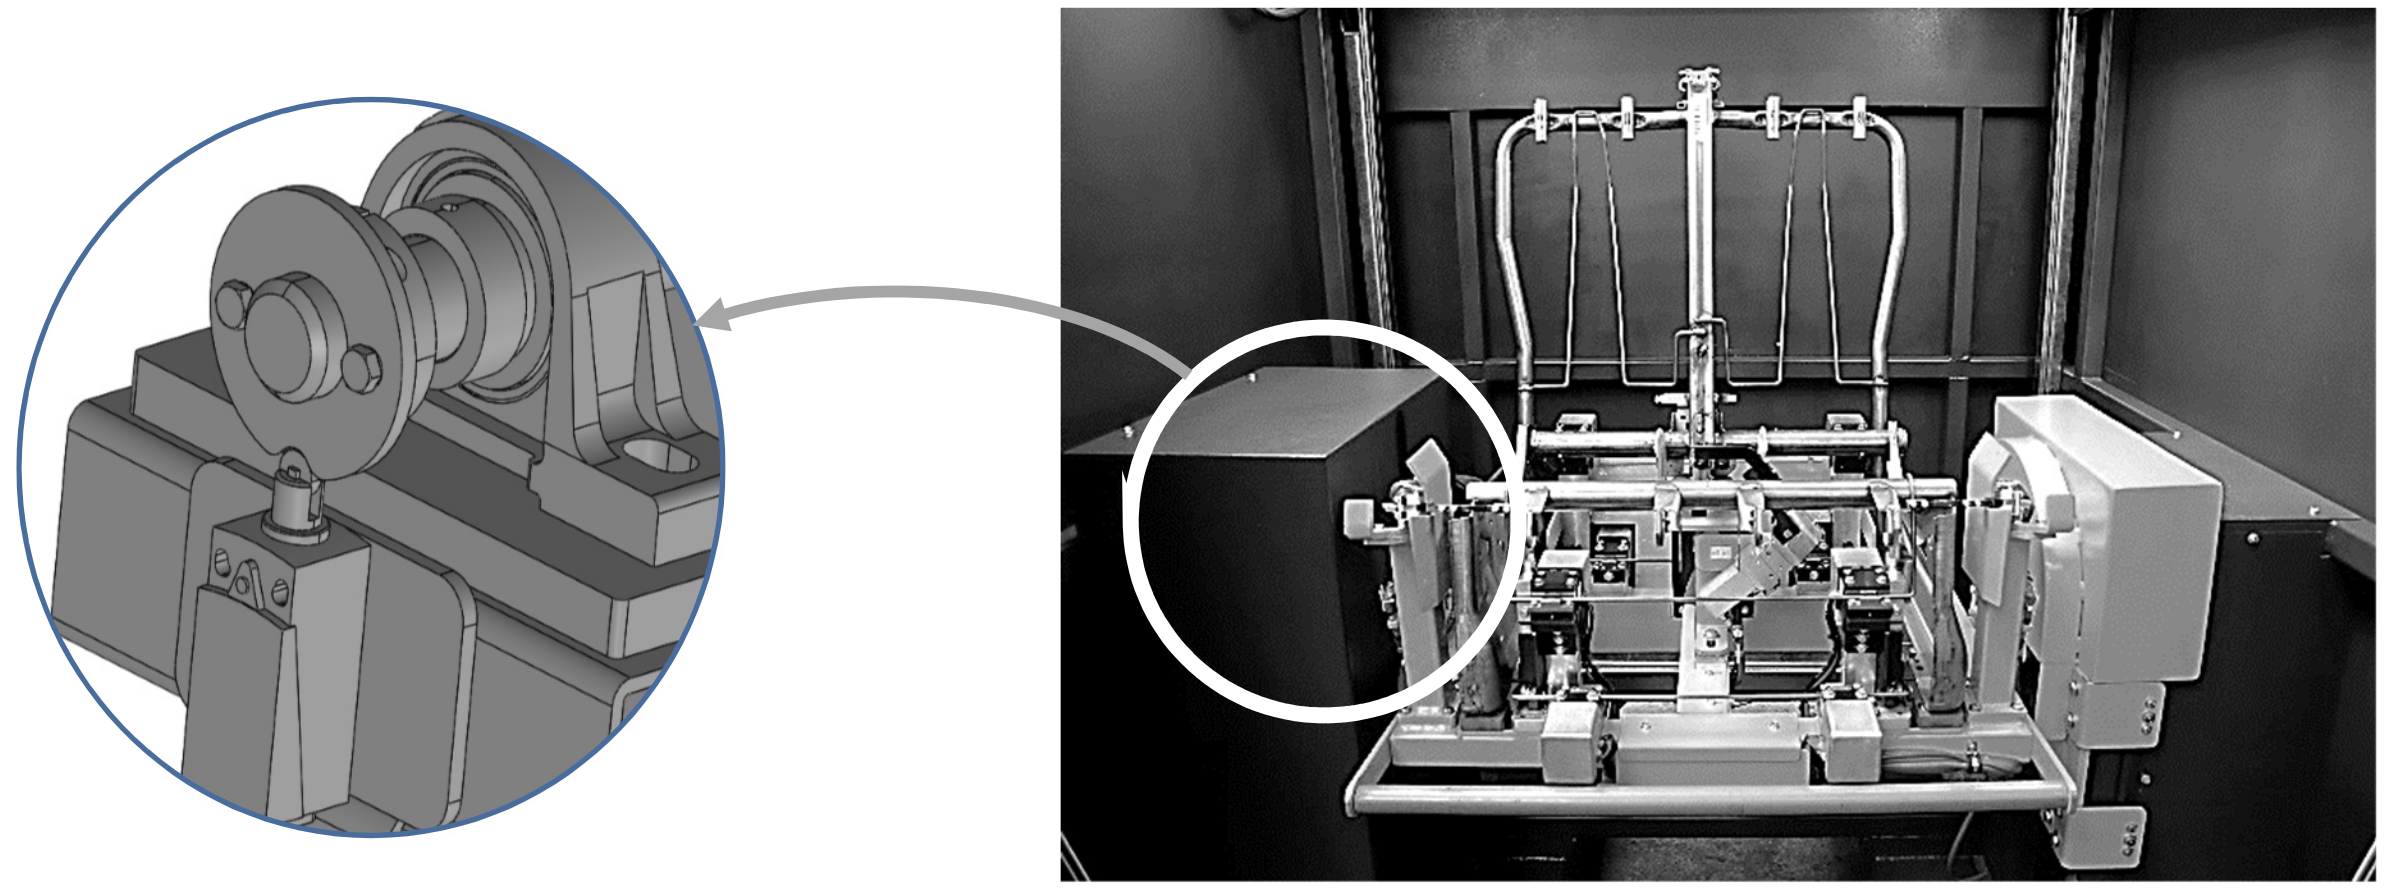
\includegraphics[width=0.8\linewidth]{img/fig07}
 \caption{Détail de la zone étudiée}
 \label{img07}
\end{figure}

On donne le schéma technologique de la solution retenue :

\begin{figure}[!h]
\centering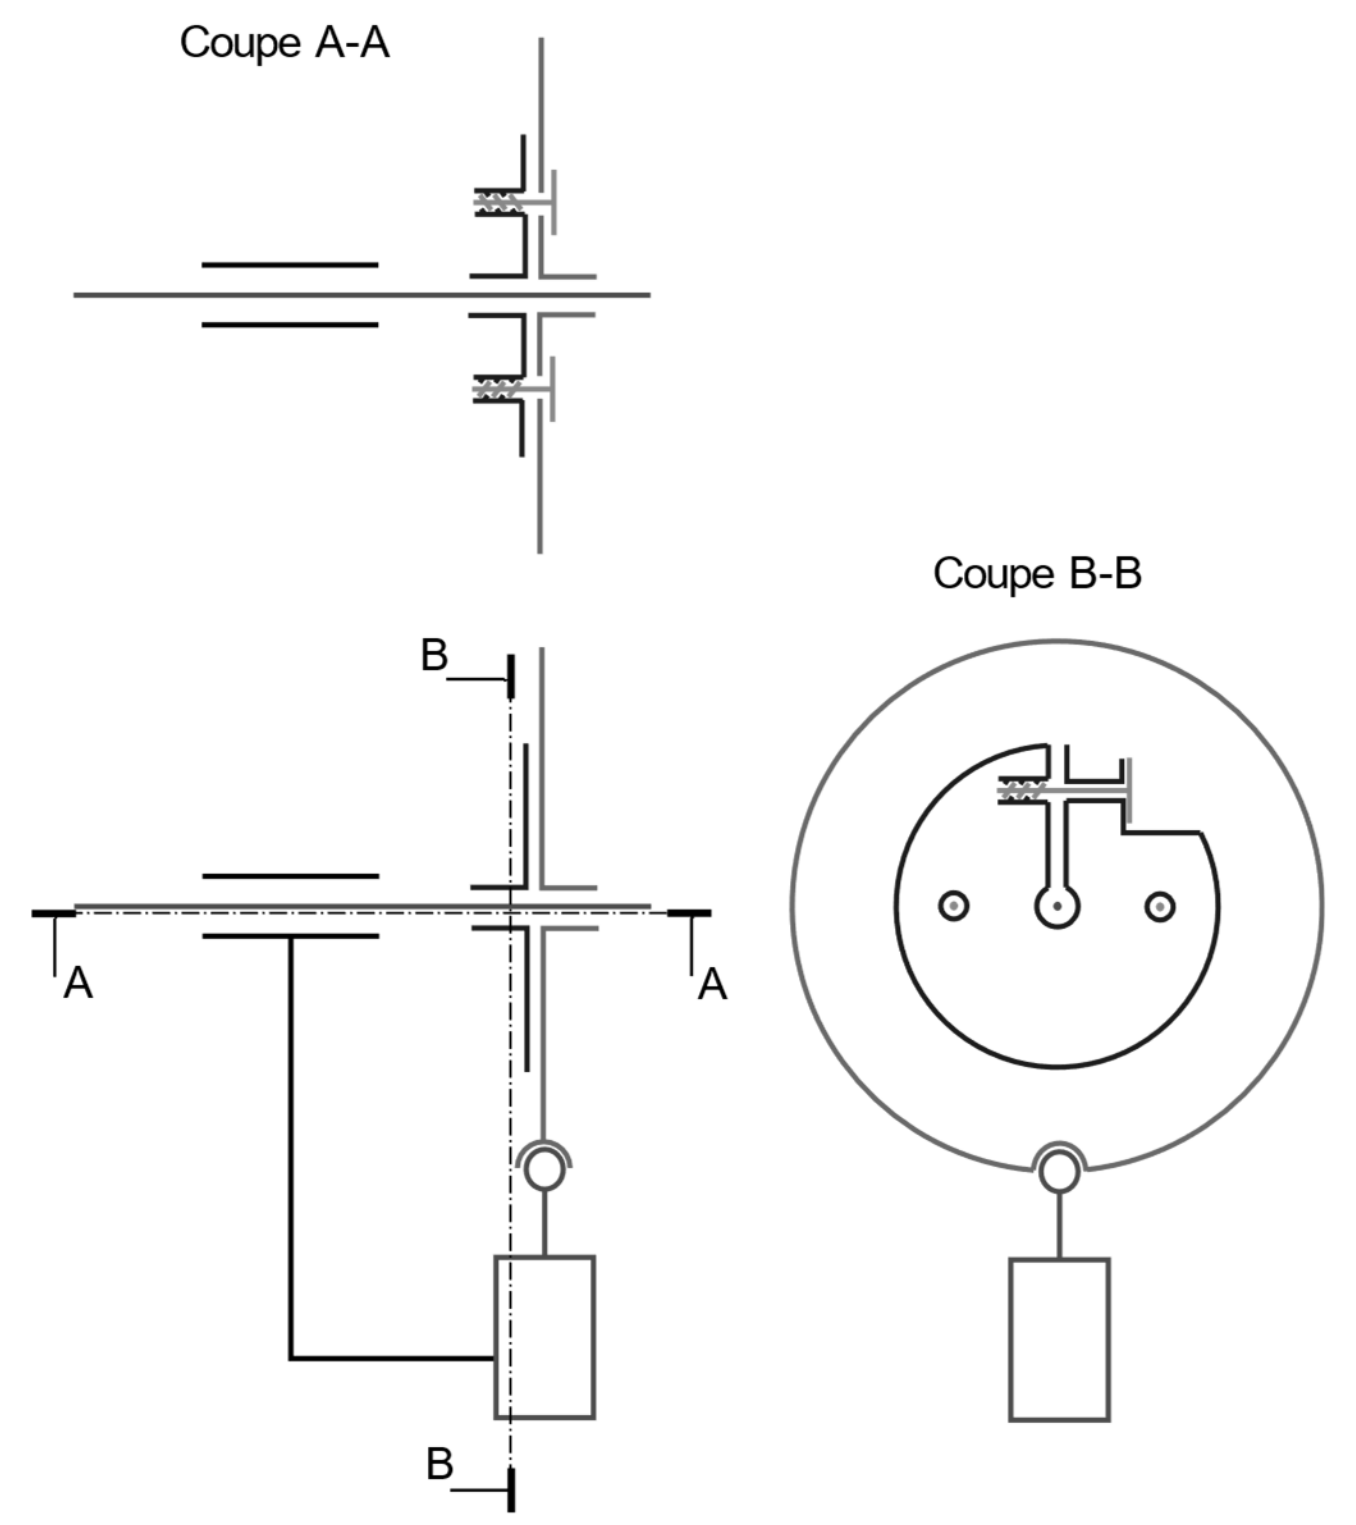
\includegraphics[width=0.45\linewidth]{img/fig08}
 \caption{Schéma technologique}
 \label{img08}
\end{figure}

\question{Compléter sur le document réponse DR1 les coupes A-A et B-B en définissant la solution d’encastrement retenue, présentée dans le schéma technologique (figure \ref{img08}).}

\question{Proposer un ajustement entre la came et l’axe au niveau de l’encastrement réalisé.}

\subsection{Étude de l’équilibrage de l’ensemble tournant}

Afin de limiter au maximum les efforts fournis par l’opérateur lors de la phase de retournement, il est nécessaire d’équilibrer statiquement l’ensemble tournant composé du berceau et du siège en positionnant une masse d’équilibrage M A (figure \ref{img09}).

\begin{figure}[!h]
\centering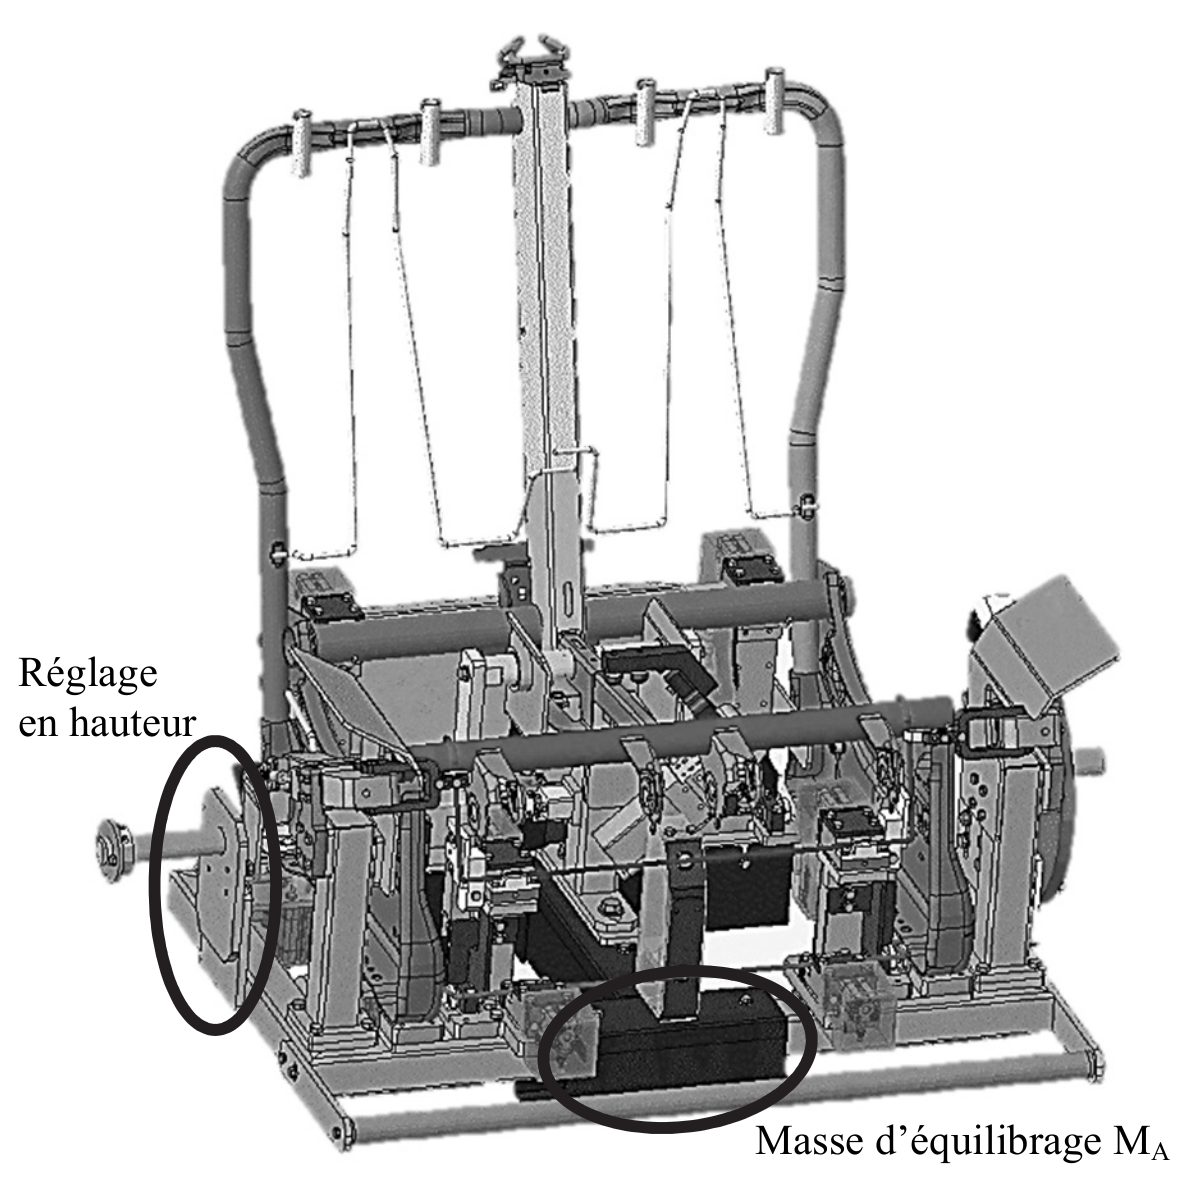
\includegraphics[width=0.45\linewidth]{img/fig09}
 \caption{Ensemble tournant à équilibrer}
 \label{img09}
\end{figure}

\question{Pour équilibrer statiquement un ensemble tournant, où doit se trouver le centre de gravité de l’ensemble ?}

~\

On propose un modèle simplifié d’étude pour lequel on connait la masse M G et la position du centre de gravité $G$ de l’ensemble tournant $E_T$ (berceau + siège) avant équilibrage statique.

\begin{figure}[!h]
\centering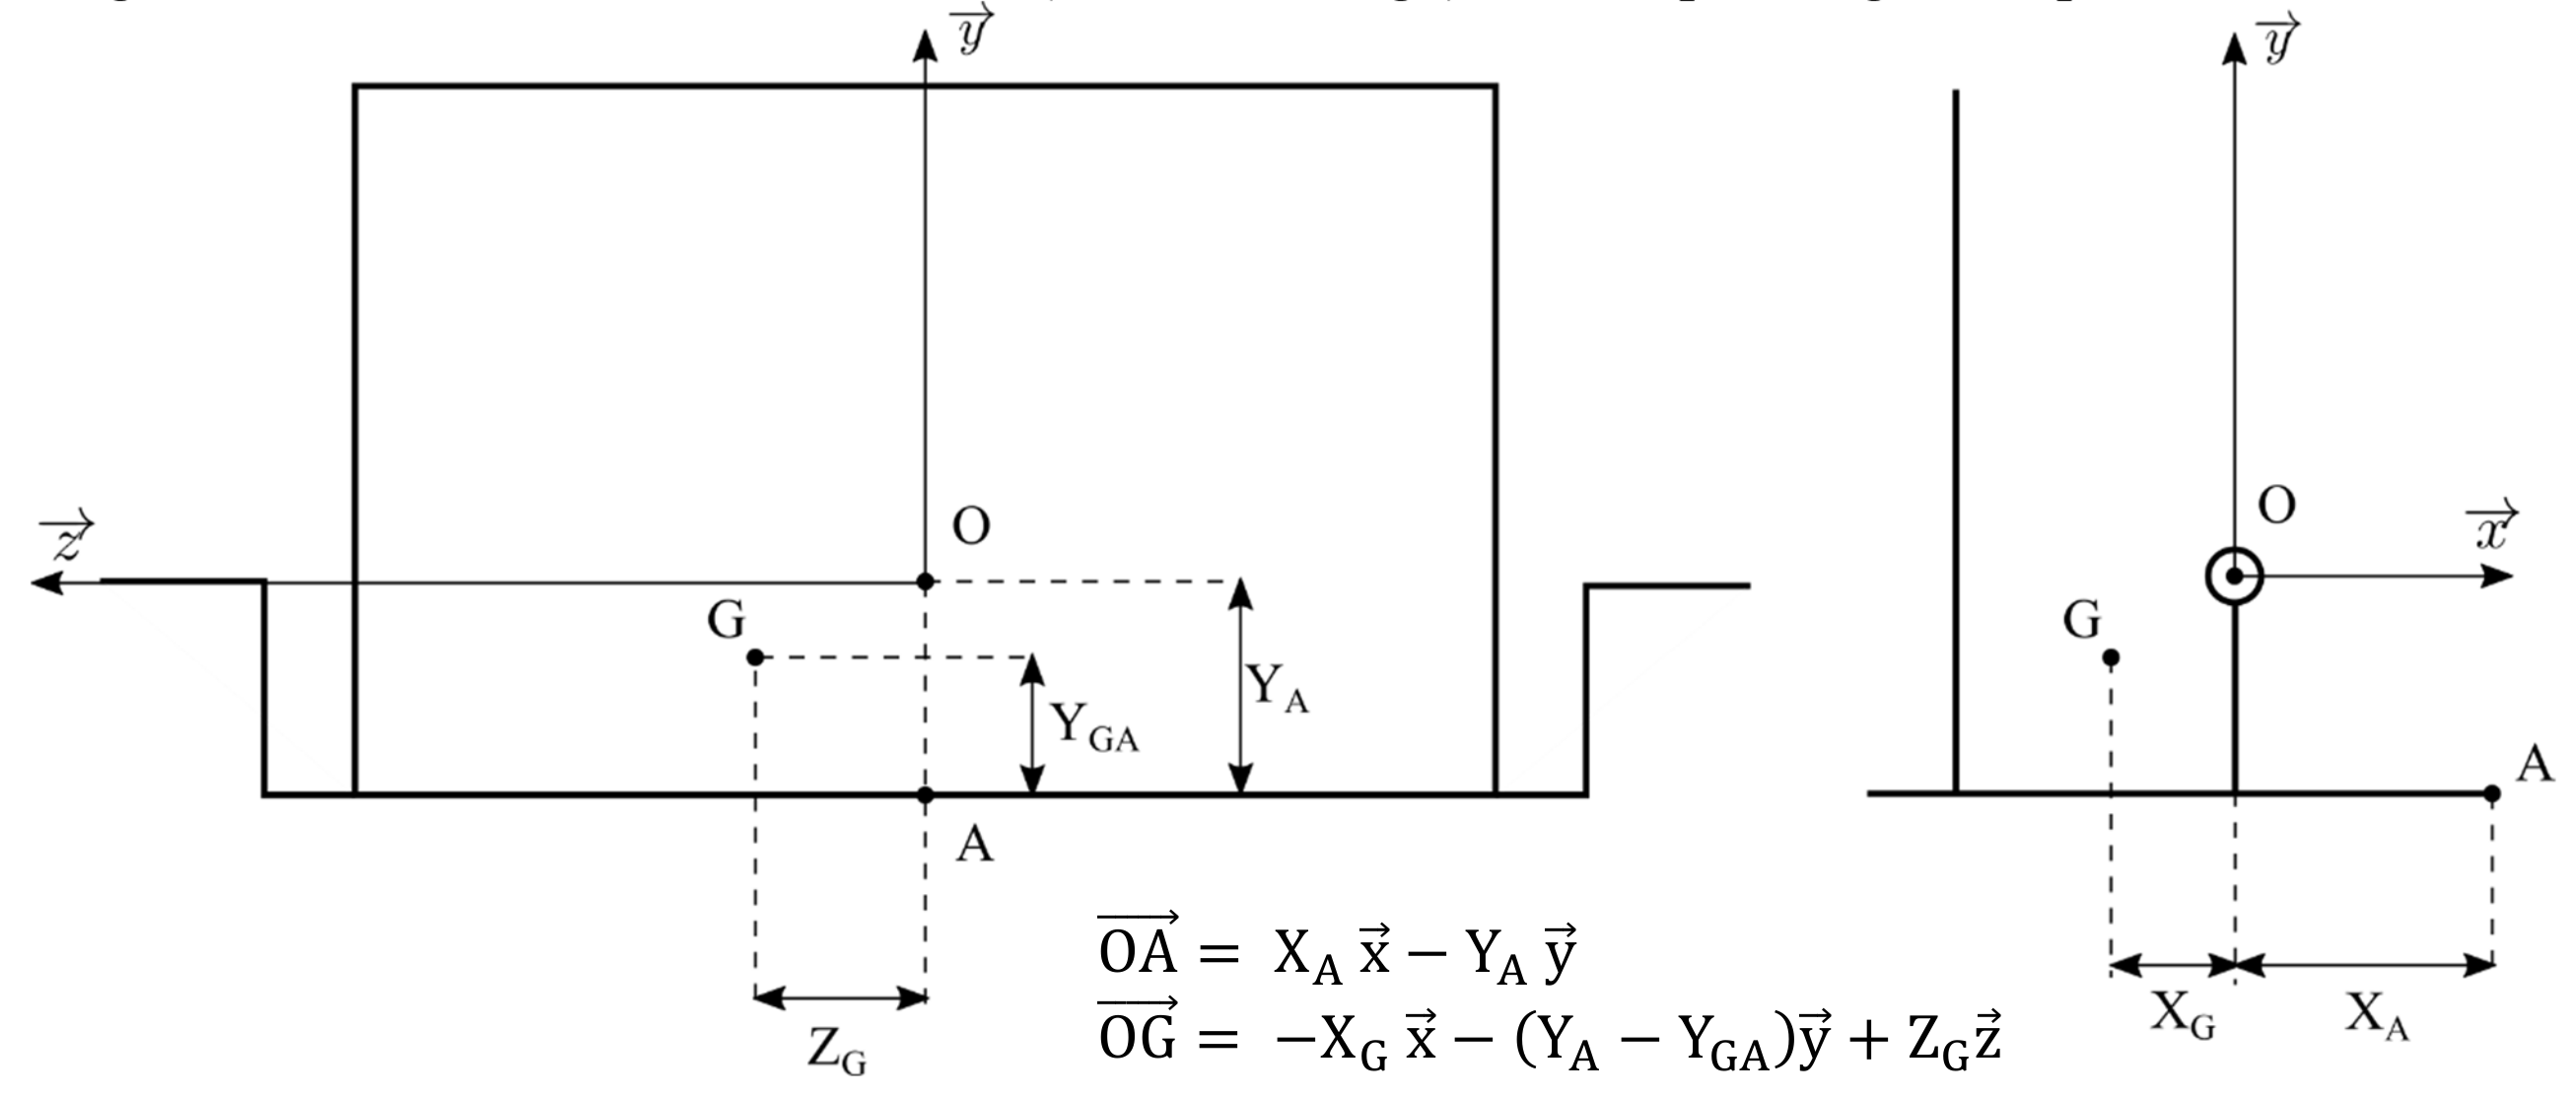
\includegraphics[width=0.8\linewidth]{img/fig10}
 \caption{Modèle simplifié pour l’étude de l’équilibrage}
 \label{img10}
\end{figure}

La solution retenue consiste à :
\begin{itemize}
 \item ajouter une masse d’équilibrage $M_A$ au point A, afin de positionner le centre de gravité $G$ dans le plan $(O,\vec{y},\vec{z})$,
 \item régler $Y_A$, hauteur suivant $\vec{y}$ du vecteur $\overrightarrow{OA}$, afin de positionner le centre de gravité sur l’axe
$(O, \vec{z})$.
\end{itemize}

On considère l’ensemble tournant dans sa position horizontale (figure \ref{img10}). Dans cette position particulière, la pesanteur est portée par la direction $\vec{y}$.

On donne la formule du barycentre:
$\overrightarrow{OG}=\frac{\sum m_i\cdot \overrightarrow{OG_i}}{\sum m_i}$

\question{En utilisant la méthode barycentrique permettant de déterminer un centre de gravité, établir les deux équations en projection sur $\vec{x}$ et $\vec{y}$ liant respectivement $X_A$, $X_G$, $M_A$, $M_G$ et $Y_A$, $Y_G$, $M_A$, $M_G$.}

\question{En déduire l’expression de M A en fonction de X A , X G et M G puis l’expression de $Y_A$ en fonction de $X_A$, $X_G$ et $Y_{GA}$.}

On note $M_{GT}$ la nouvelle masse et $G_T$ le nouveau centre de gravité de l’ensemble $E_T$.

\question{Donner l’expression de $M_{GT}$ en fonction de $M_G$ et de $M_A$. Donner les coordonnées ($X_{GT}$; $Y_{GT}$; $Z_{GT}$) du nouveau centre de gravité $G_T$ de l’ensemble tournant $E_T$.}

\section{Exigence \og Brider le siège et les fils \fg}

\subsection{Étude de la genouillère de bridage}

La genouillère de bridage permet de maintenir en position le siège sur le berceau de soudage (figure \ref{img11} et \ref{img12}).

\begin{figure}[!h]
\centering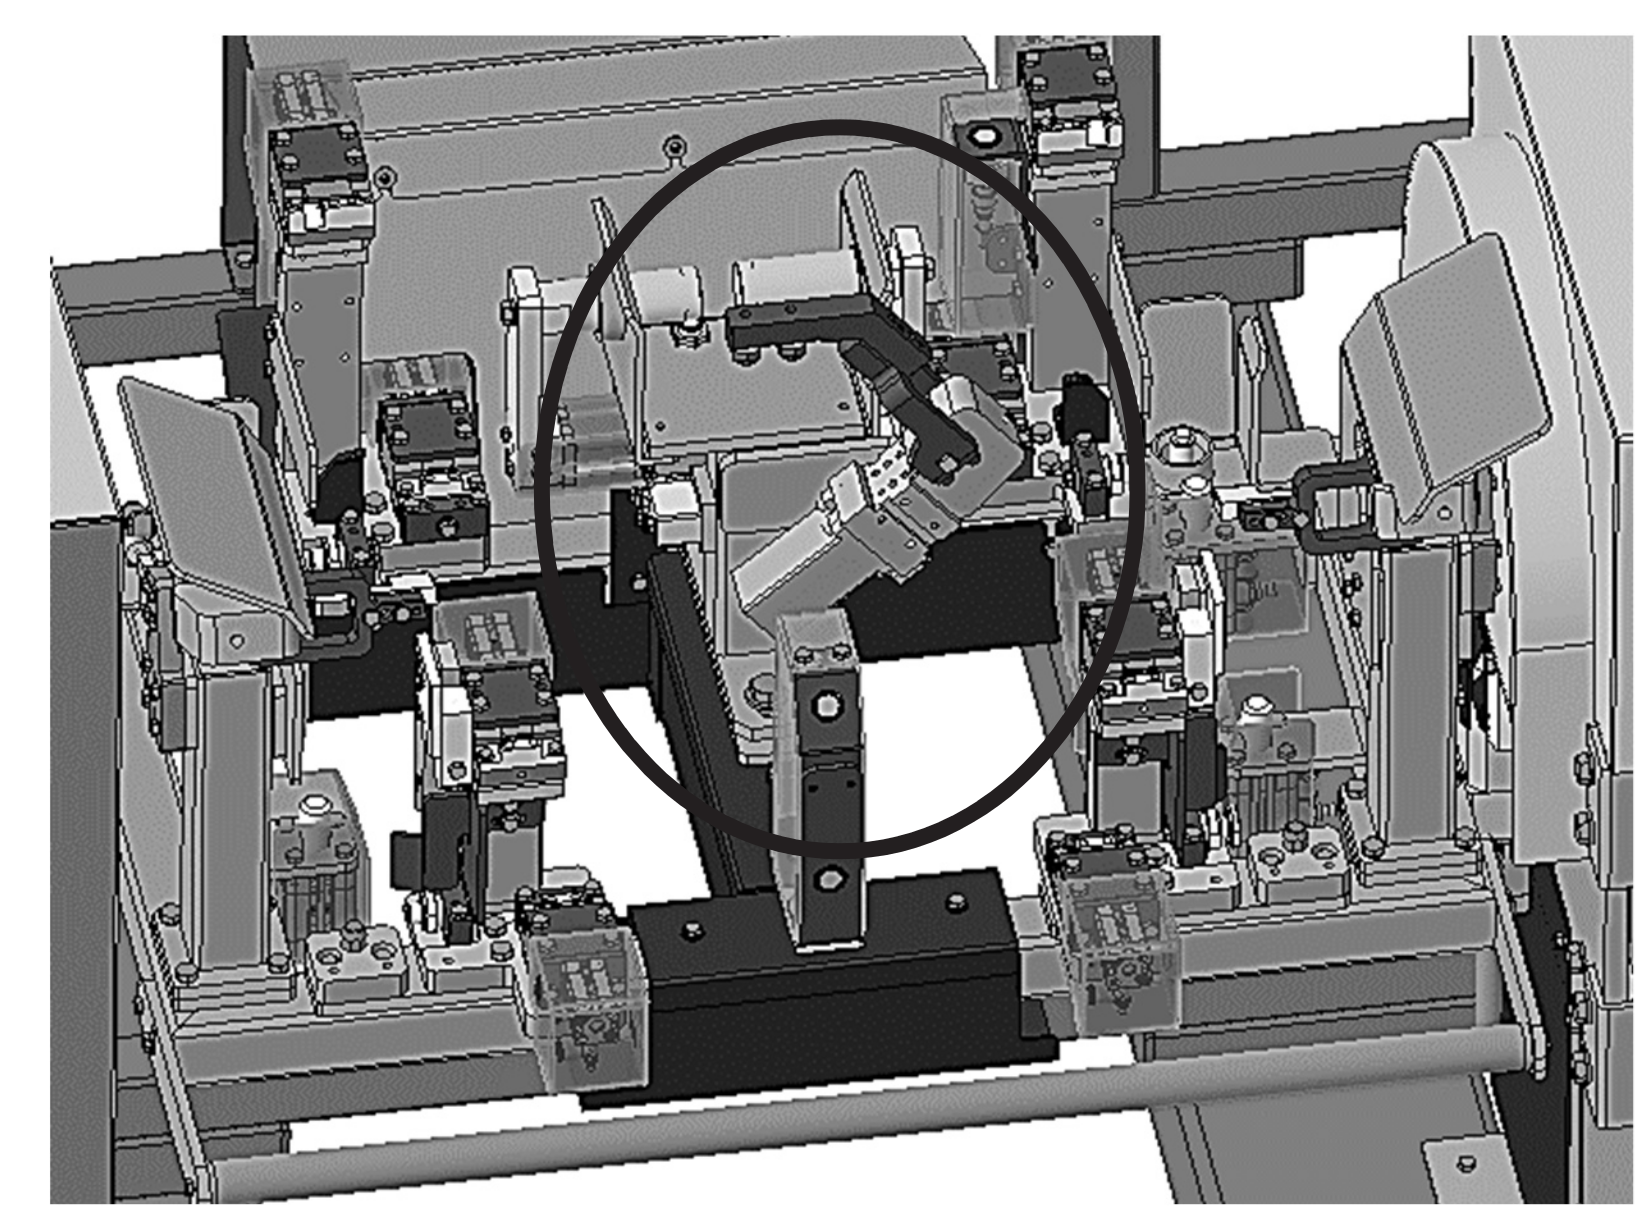
\includegraphics[width=0.7\linewidth]{img/fig11}
 \caption{Genouillère en situation}
 \label{img11}
\end{figure}

\begin{figure}[!h]
\centering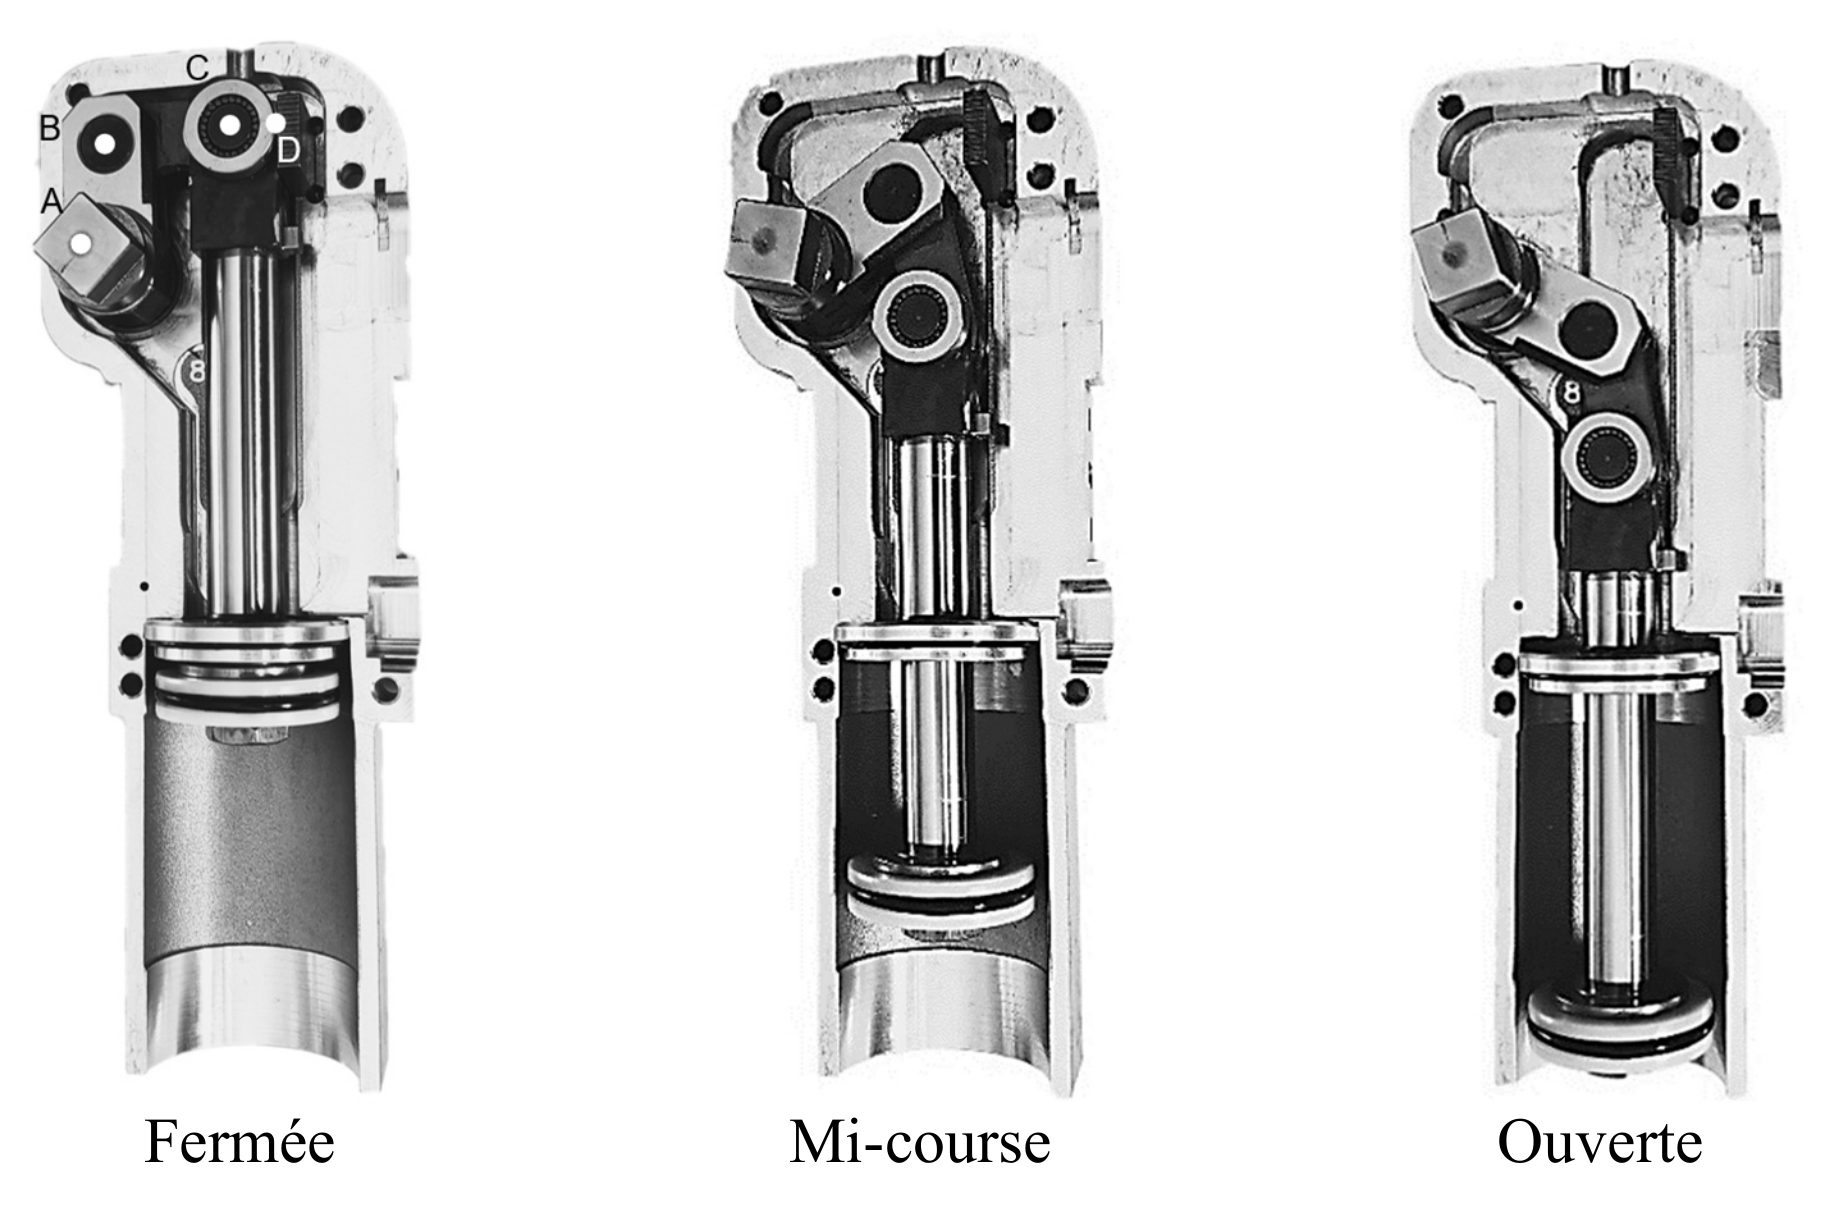
\includegraphics[width=0.6\linewidth]{img/fig12}
 \caption{Positions de la genouillère}
 \label{img12}
\end{figure}

\newpage

Le schéma cinématique plan de la genouillère de bridage utilisée dans le système est donné figure \ref{img13}.

Le paramétrage décrit ci-dessous sera utilisé :
\begin{itemize}
 \item le solide \textbf{1} est en translation de direction $\vec{y}_0$,
 \item le solide \textbf{2} est en rotation d'axe $(E,\vec{z})$ avec le solide \textbf{1}. On pose: $\alpha=(\vec{x}_1,\vec{x}_2)$,
 \item le solide \textbf{3} est en rotation d'axe $(D,\vec{z})$ avec le solide \textbf{2},
 \item le solide \textbf{3} est en rotation d'axe $(C,\vec{z})$ avec le solide \textbf{0}. On pose: $\beta=(\vec{x}_1,\vec{x}_3)$,
 \item $\overrightarrow{CD}=l_3\cdot\vec{x}_3$, $\overrightarrow{DE}=-l_2\cdot\vec{y}_2$, $\overrightarrow{EF}=l_1\cdot\vec{x}_1$, $\overrightarrow{OE}=\lambda\cdot\vec{y}_0$ et $\overrightarrow{OC}=l_x\cdot\vec{x}_0+l_y\cdot\vec{y}_0$.
\end{itemize}

\begin{figure}[!h]
\centering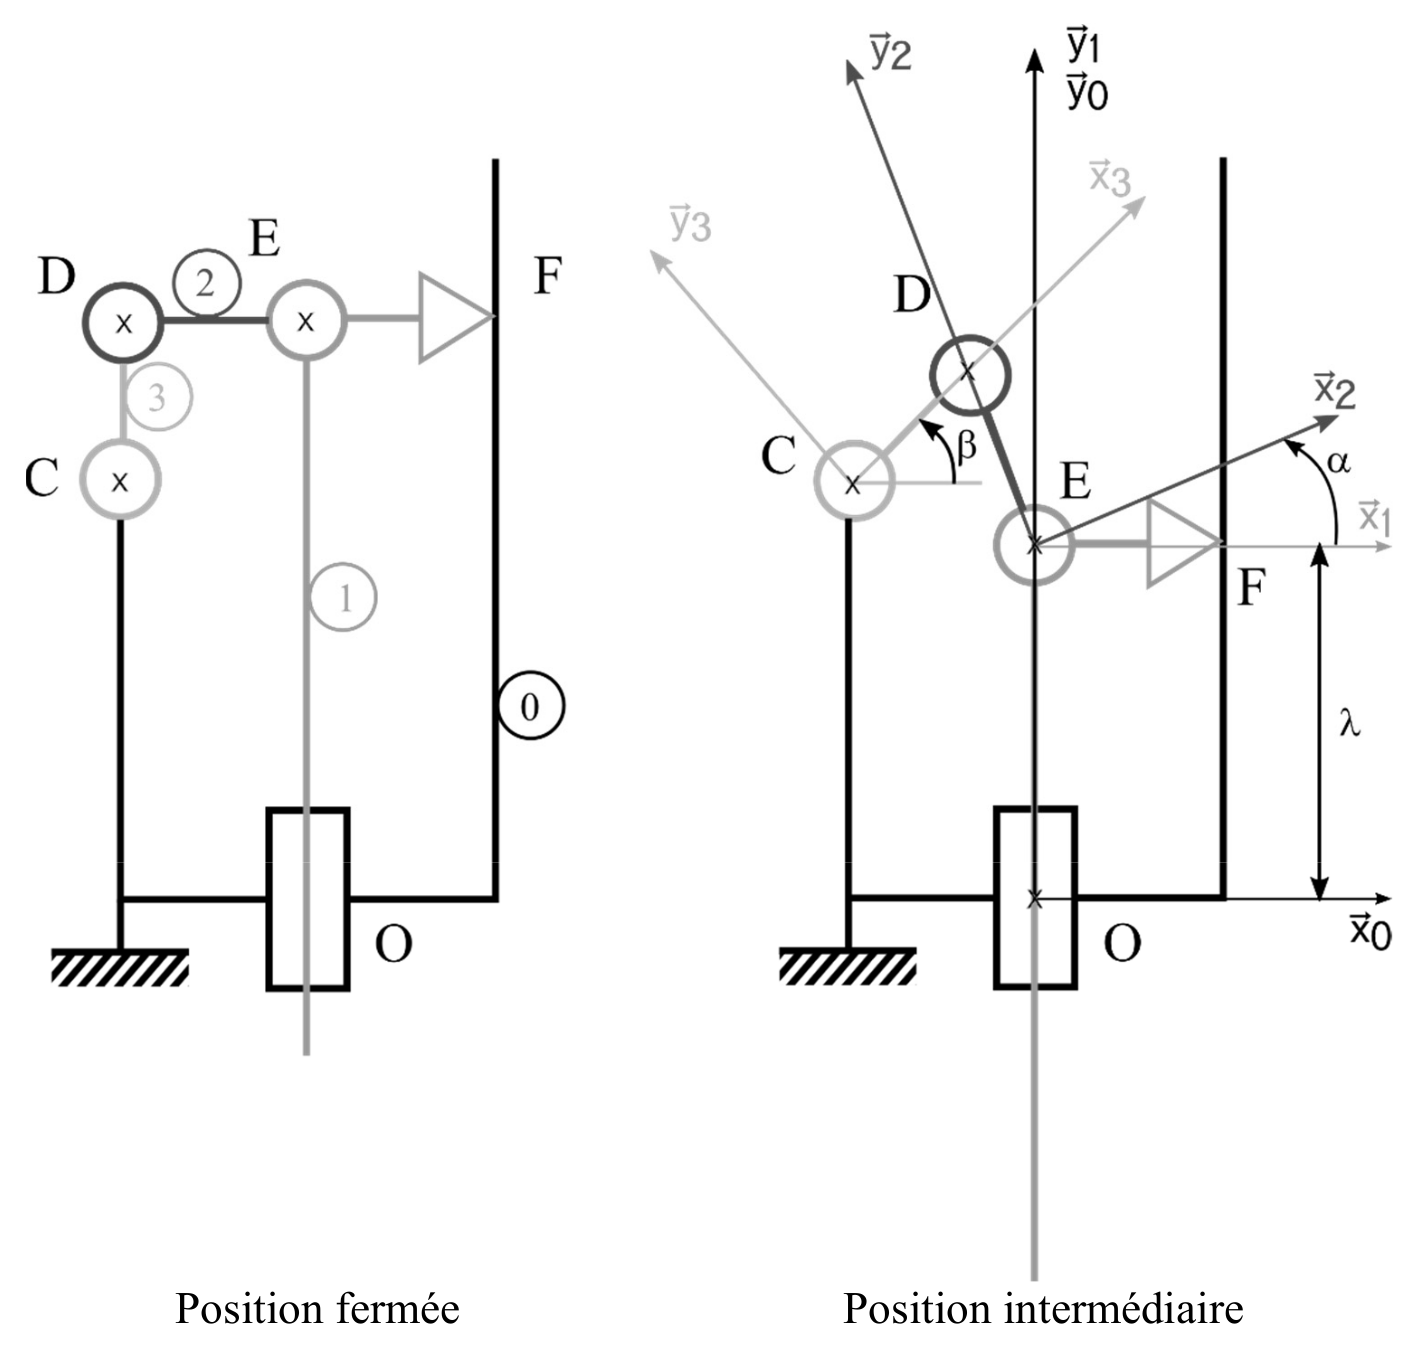
\includegraphics[width=0.65\linewidth]{img/fig13}
 \caption{Schéma cinématique de la genouillère}
 \label{img13}
\end{figure}

\question{Écrire la fermeture géométrique permettant de déterminer la loi entrée/sortie de la genouillère.}

\question{Projeter cette équation vectorielle dans le repère $R_0(O,\vec{x}_0,\vec{y}_0,\vec{z}_0)$.}

\question{En déduire une relation entre $\beta$ et $\lambda$.}

Afin de garantir un bridage irréversible, il faut que les 3 points D, E, F soient alignés, comme le montrent les positions fermées des figures \ref{img12} et \ref{img13}. Dans cette configuration particulière, le piston n’est soumis à aucune action mécanique verticale.

\question{En réalisant une étude statique simple, justifier que dans le cas où les 3 points D, E et F sont alignés, le piston \textbf{1} n’est soumis à aucune action mécanique extérieure selon la direction
$\vec{y}_0$.}
-
\subsection{Étude pneumatique}

La cabine de soudure dispose d’une genouillère de bridage, de différents vérins d’indexation et d’une alimentation pneumatique. Tous ces dispositifs utilisent le même type de distributeur.

\begin{figure}[!h]
\centering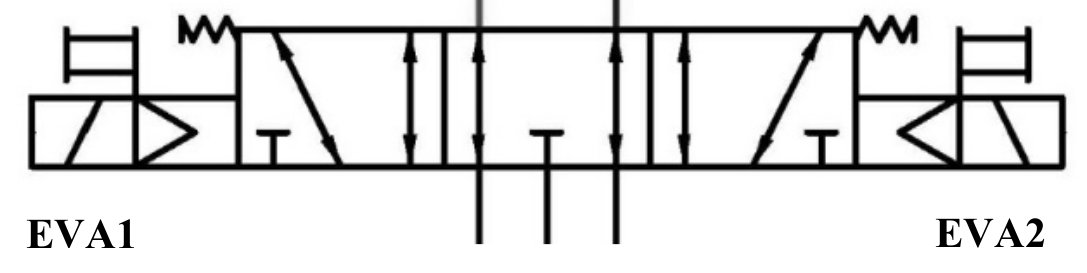
\includegraphics[width=0.4\linewidth]{img/fig14}
 \caption{Distributeur utilisé pour le bridage}
 \label{img14}
\end{figure}

\question{Donner la désignation normalisée de ce distributeur (figure \ref{img14}).}

\question{Compléter le schéma pneumatique des deux ensembles brides A et B sur le DR2. Le distributeur A permet d’actionner la bride A1 et les 2 brides A2.

Le distributeur B permet d’actionner les deux brides B1.}

\subsection{Étude électrique}

On souhaite dimensionner l’alimentation électrique de la cabine de soudure. Le schéma électrique unifilaire d’alimentation de la cabine de soudage est fourni en annexe 2.

\question{Pour quelle raison est-il nécessaire d’utiliser le transformateur T0508 ?
D’autres solutions seraient-elles possibles ?}

~\

On souhaite dimensionner ce transformateur. Pour cela, il est nécessaire de faire un bilan des puissances consommées par l’ensemble des récepteurs. On considérera le facteur de puissance de chaque récepteur \og $cos \varphi$ \fg\ et les rendements des convertisseurs égaux à 1.

La puissance et les courants maximums de tous les récepteurs sont indiqués sur le schéma électrique en annexe 2.

On tiendra compte d’une prévision d'évolution de l’ensemble des charges de + 20\%.

\question{Déterminer la puissance apparente S, en VA, du transformateur à installer.}

\subsection{Étude de la partie commande}

On donne en annexe 3 le graphe d’état de fonctionnement normal du système.

\question{Compléter les chronogrammes d’évolution du système sur le DR3.}

~\

On souhaite ajouter un état \og défaut de bridage \fg lorsque le bridage A, B, ou C n’est pas validé.

Pour sortir de l’état \og défaut de bridage \fg, il sera nécessaire d’appuyer sur DCY afin de passer dans l’état \og Remise à l’état initial \fg.

\question{Compléter, sur le DR6, le graphe d’état \og fonctionnement \fg en ajoutant l’état \og défaut de bridage \fg et les transitions associées.}

\section{Exigence \og Positionner en hauteur \fg}

Le réglage en hauteur du berceau permet d’adapter le poste de travail à la morphologie de chaque opérateur (figure \ref{img16}).

\begin{figure}[!h]
\centering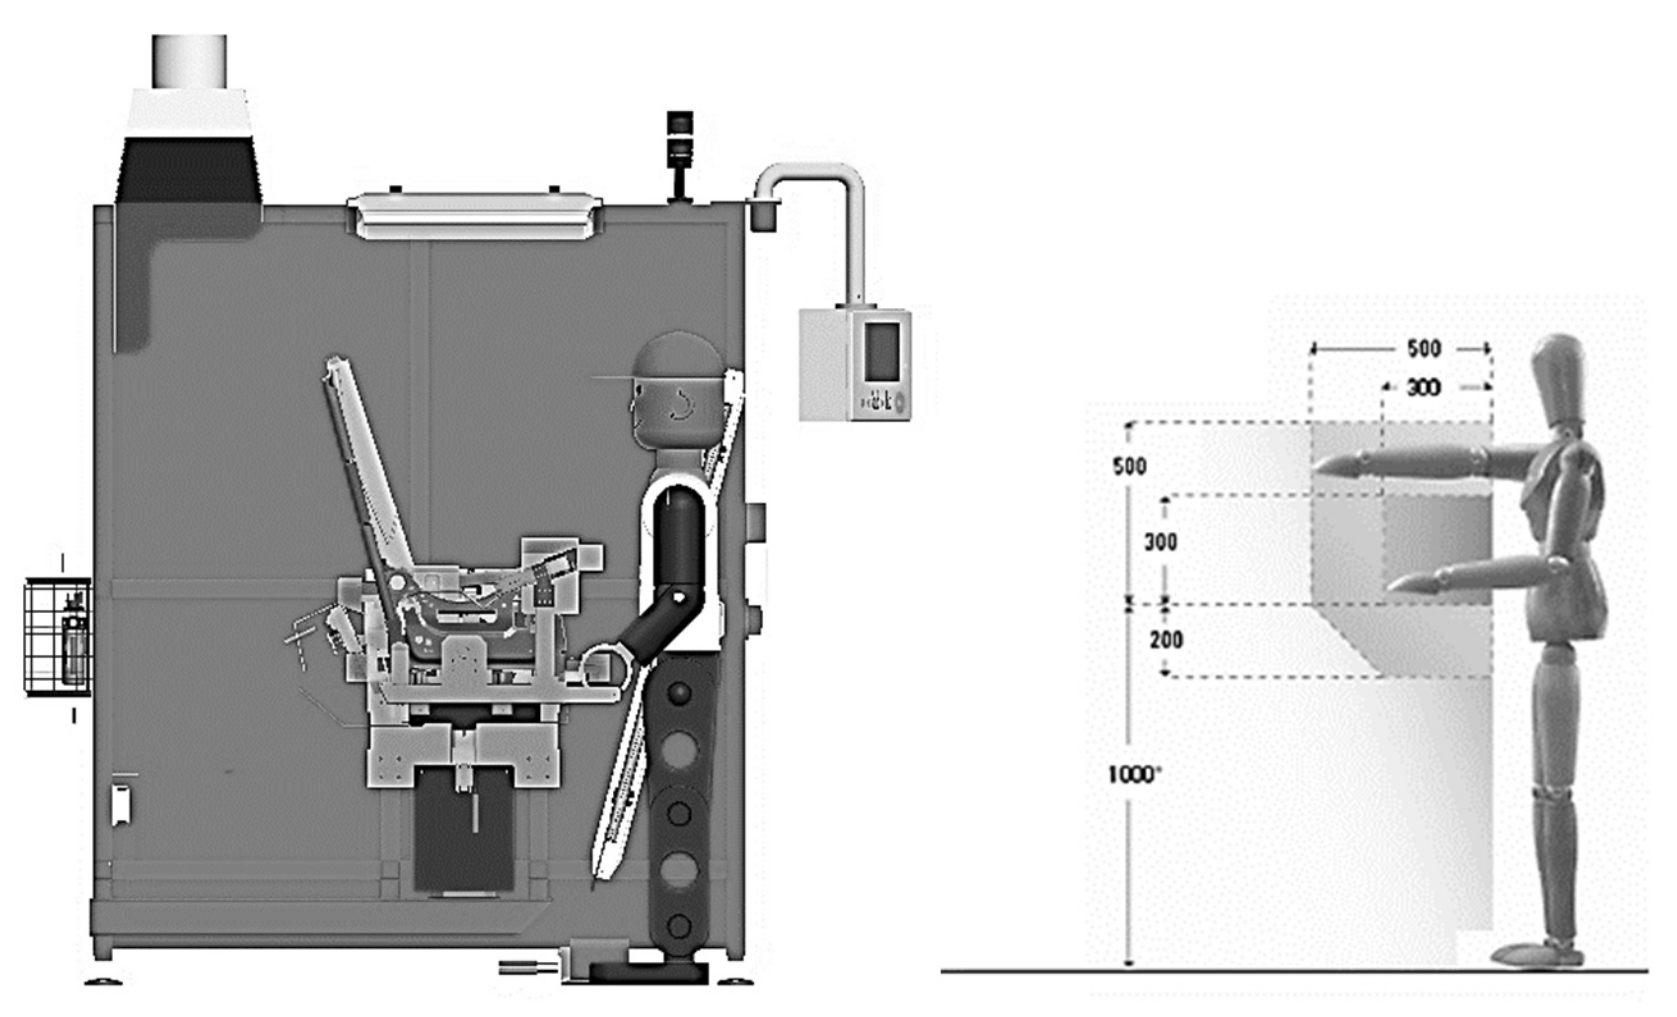
\includegraphics[width=0.7\linewidth]{img/fig16}
 \caption{Position préconisée}
 \label{img16}
\end{figure}

L’opérateur règle la hauteur de son poste de travail en appuyant sur les boutons \og haut \fg ou \og bas \fg positionnés à sa droite.

Le réglage de cette hauteur est réalisé par deux vérins linéaires électriques dont les positions sont asservies l’une par rapport à l’autre.

\subsection{Horizontalité du poste de travail}

Pendant toute la phase de mouvement, le poste de travail doit rester horizontal afin de ne pas forcer sur les deux liaisons glissières, droite et gauche et sur les vérins linéaires électriques.

La hauteur de chaque vérin est notée $\lambda$ et $\lambda'$ (figure \ref{img17}). On notera $\Delta\lambda=(\lambda-\lambda')$ l’écart de
longueur de sortie des tiges des vérins droit et gauche. La distance entre les centres I et J des guidages verticaux, notée $L$, est égale à $1 000 mm$.

\newpage

\begin{figure}[!h]
\centering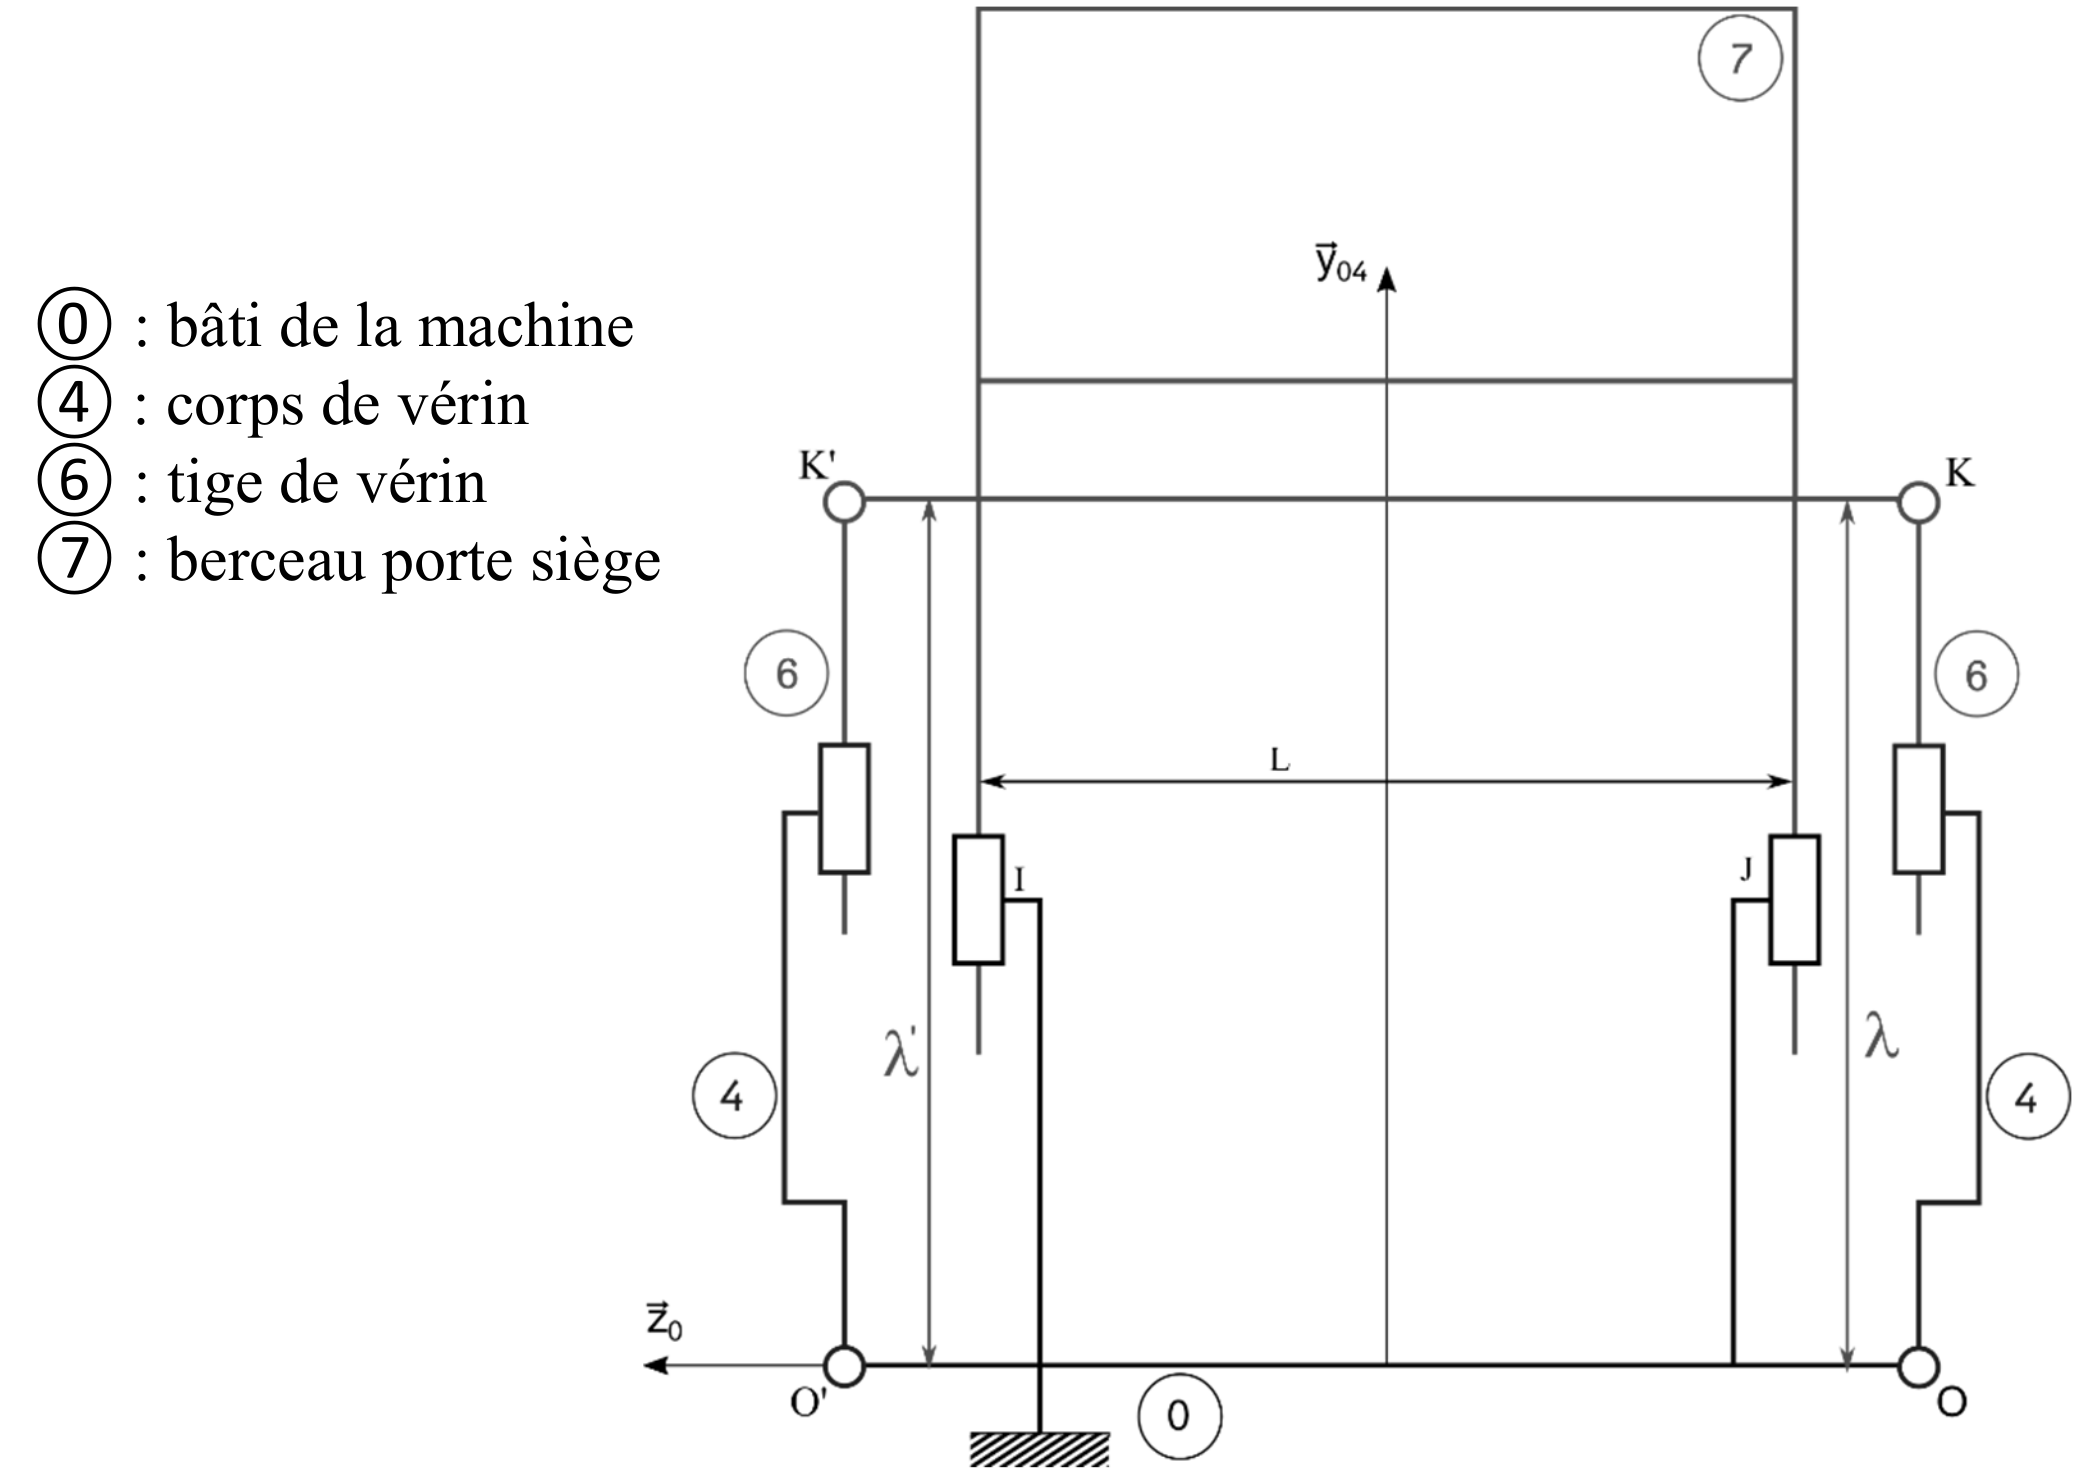
\includegraphics[width=0.6\linewidth]{img/fig17}
 \caption{Schéma cinématique du système de réglage de la hauteur}
 \label{img17}
\end{figure}

\question{Déterminer l’écart de longueur maximum $\Delta\lambda_{max}$ acceptable pour que la table garde un angle d’inclinaison inférieur à $0,1\degree\ $ qui sera absorbé par le jeu existant dans les liaisons glissières.}

~\

Afin d’assurer un écart de longueur entre les deux vérins compatibles avec l’inclinaison maximum tolérée, il faudra garantir un positionnement des vérins aux alentours du millimètre.

\subsection{Étude structurelle}

On souhaite étudier la structure du système mécanique.

Il est donc nécessaire de modéliser l’ensemble \og vérins + (berceau + siège + fils) \fg pour obtenir une commande optimale.

Soit le schéma simplifié de cet ensemble :

\begin{figure}[!h]
\centering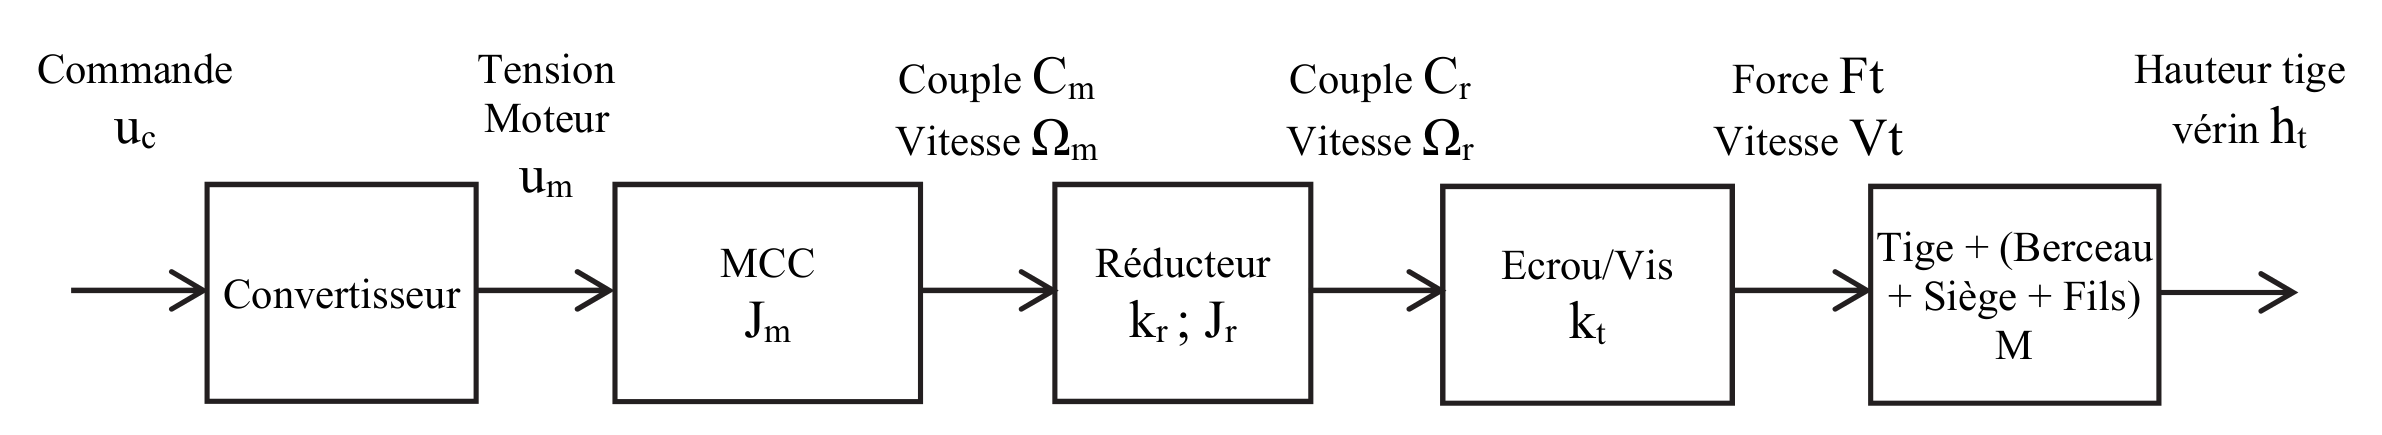
\includegraphics[width=0.8\linewidth]{img/fig18}
 \caption{Schéma fonctionnel d’un vérin linéaire et de sa charge}
 \label{img18}
\end{figure}

On définit les grandeurs caractéristiques suivantes : \\ ~\ 

\begin{minipage}{0.48\linewidth}
\begin{itemize}
 \item $u_c$ : tension de commande,
 \item $u_m$ : tension d’alimentation du moteur,
 \item $C_m$ : couple moteur,
 \item $\Omega_m$ : vitesse angulaire moteur,
 \item $C_r$ : couple en sortie de réducteur,
 \item $\Omega_r$ : vitesse angulaire réducteur,
 \item $F_t$ : force de poussée du vérin,
 \item $V_t$ : vitesse de sortie du vérin,
\end{itemize}
\end{minipage}\hfill
\begin{minipage}{0.48\linewidth}
\begin{itemize}
 \item $J_m$ : inertie moteur,
 \item $k_r$ : rapport de réduction,
 \item $J_r$ : inertie du réducteur sur son arbre de sortie,
 \item $k_t$ : rapport de transmission écrou/vis,
 \item $M$ : masse de l’ensemble tige + (berceau + siège
+ fils).
\end{itemize}
\end{minipage}

~\

Nous allons étudier le mouvement de la masse mobile (berceau + siège + fils) et déterminer son degré d'hyperstatisme afin d'anticiper d'éventuels problèmes d'assemblage.

\begin{figure}[!h]
\centering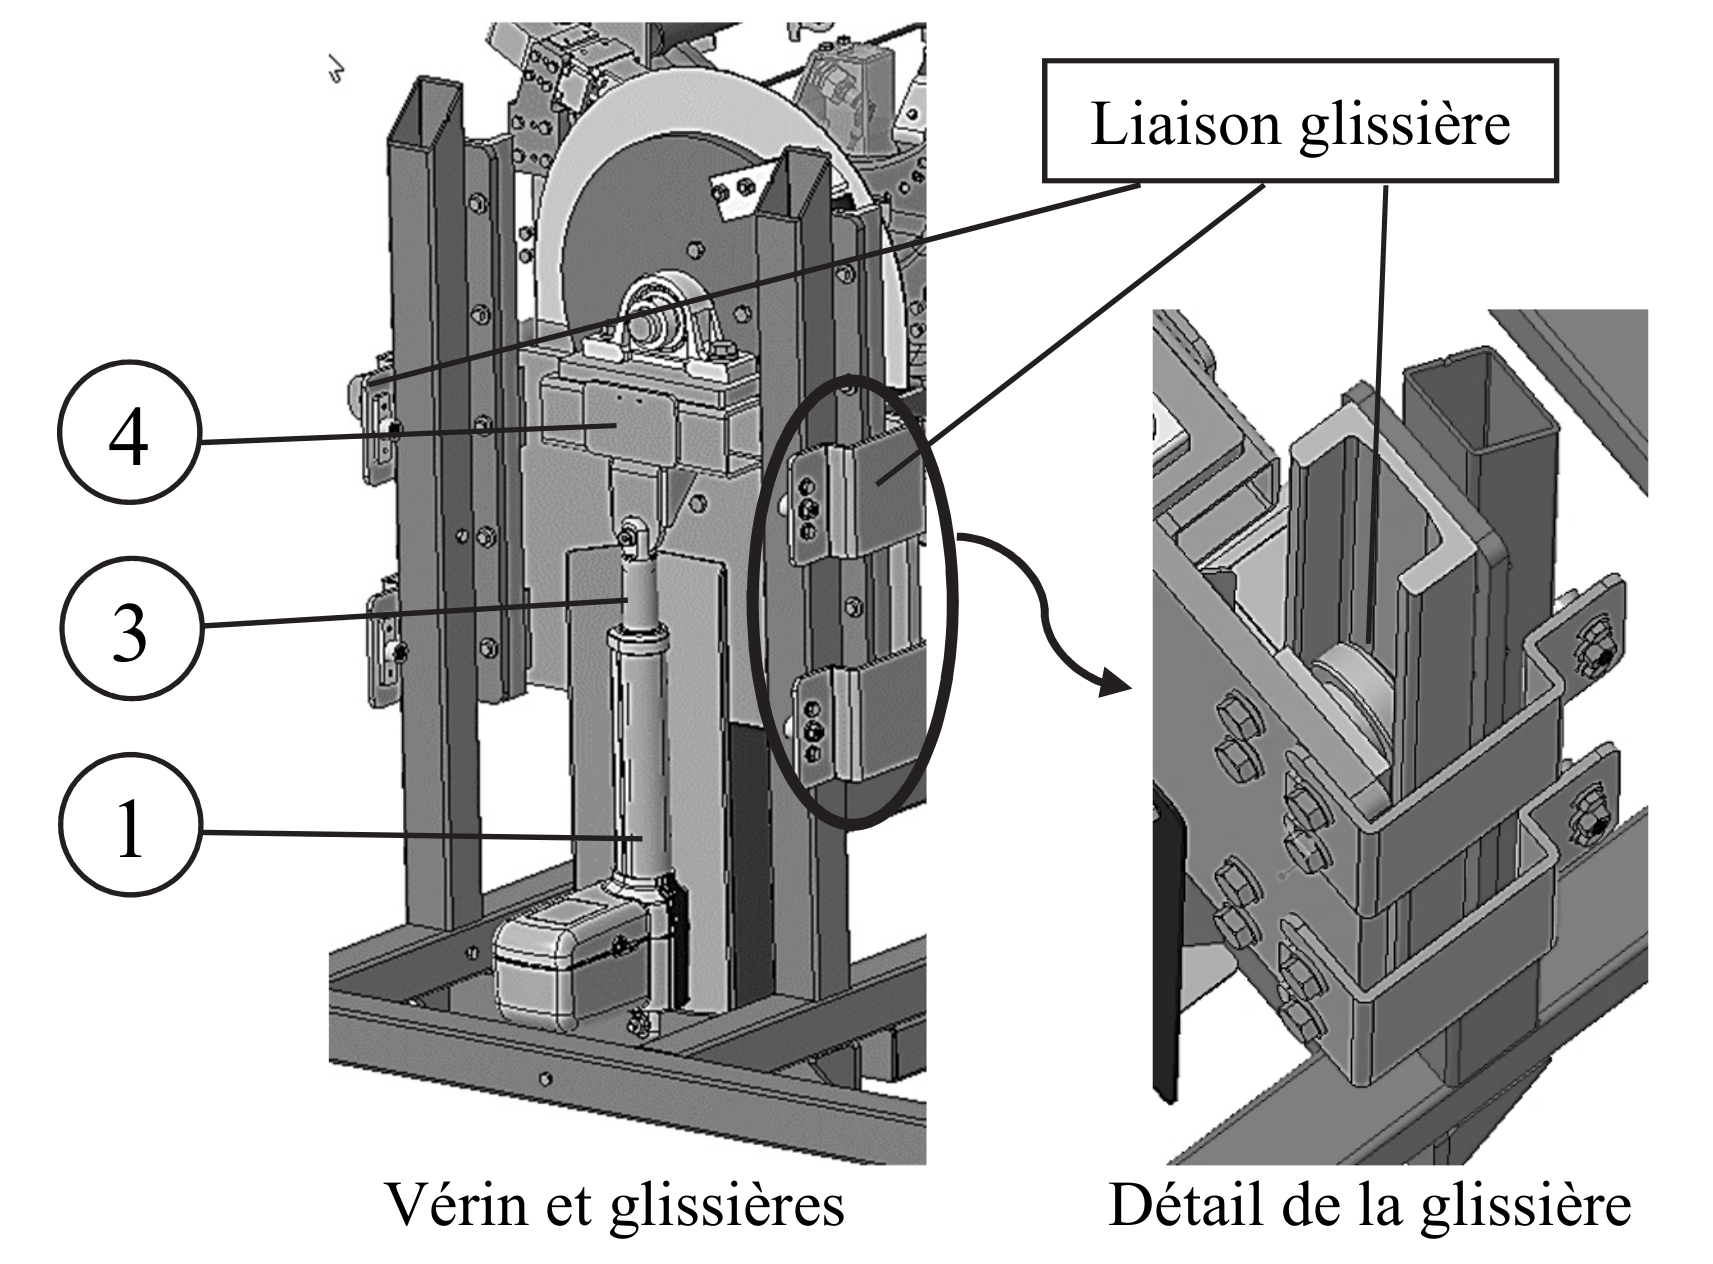
\includegraphics[width=0.6\linewidth]{img/fig19}
 \caption{Système de levage}
 \label{img19}
\end{figure}

Le berceau ayant été équilibré statiquement afin de faciliter sa rotation, on choisit de simplifier l’étude en se ramenant à un mécanisme plan composé de deux liaisons glissières et d’un vérin (figures \ref{img19} et \ref{img20}).

On fera l’hypothèse que toutes les liaisons sont parfaites.

\begin{figure}[!h]
\centering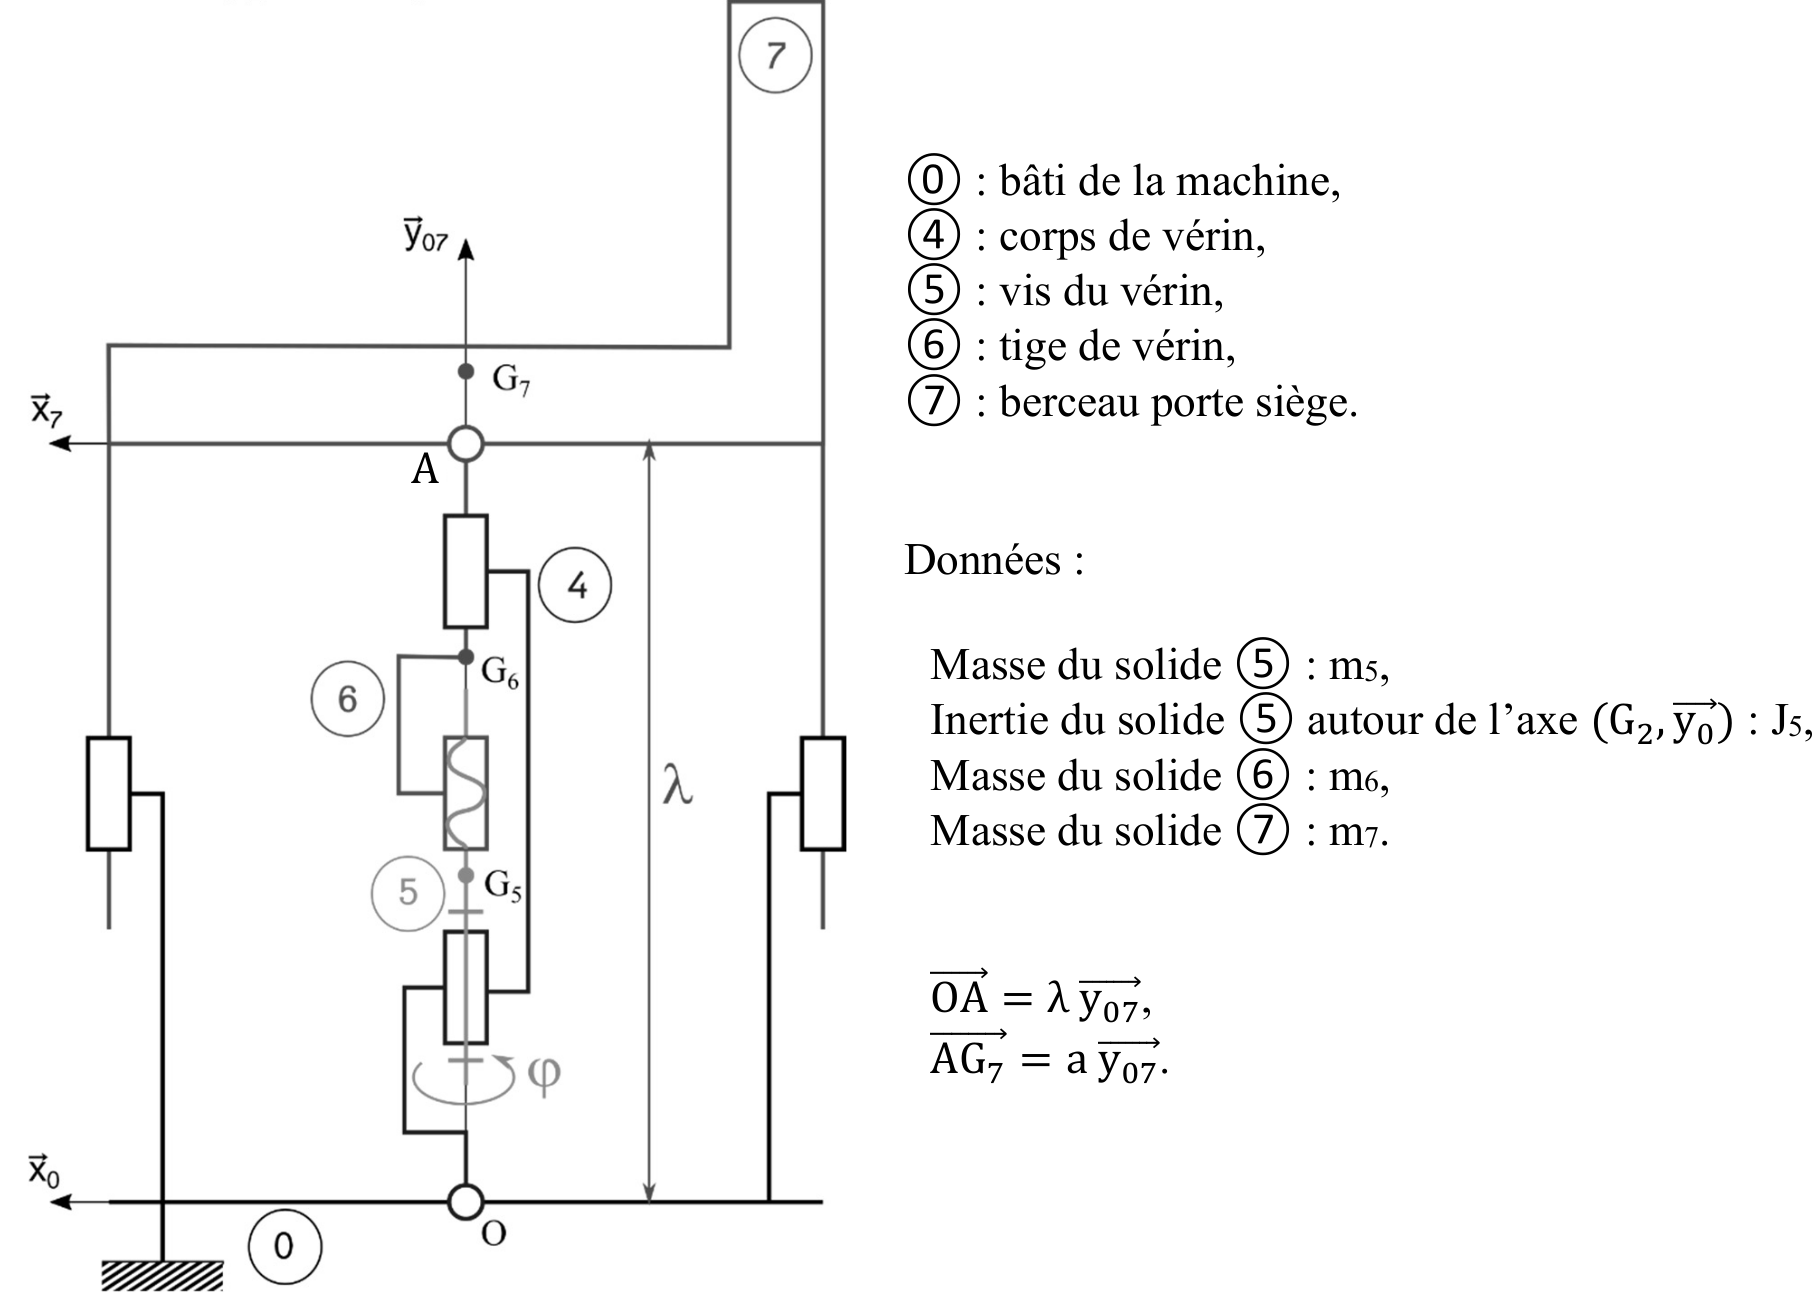
\includegraphics[width=0.8\linewidth]{img/fig20}
 \caption{Schéma cinématique simplifié du réglage de hauteur}
 \label{img20}
\end{figure}

\question{Réaliser le graphe de liaison complet de ce modèle incluant les numéros de pièces, le nom des liaisons, leurs directions/axes...}

\question{Déterminer le degré d'hyperstatisme du modèle cinématique présenté à la figure \ref{img20}.}

\question{Proposer une modification de modèle permettant de diminuer ce degré d'hyperstatisme sans ajouter de mobilité.}

\subsection{Modélisation du moteur à courant continu du vérin.}

\question{Proposer un schéma électrique de l’induit du Moteur à Courant Continu (M.C.C.) en faisant apparaître :}

\begin{itemize}
 \item $R$ : résistance de l’induit [$\Omega$],
 \item $L$ : inductance de l’induit [$H$],
 \item $e(t)$ : la force contre électromotrice [$V$],
 \item $u_m(t)$ : tension aux bornes de l’induit [$V$],
 \item $i_m(t)$ : courant induit du moteur [$A$].
\end{itemize}

\question{Donner l’équation électrique des grandeurs instantanées de ce moteur : tension $u_m(t)$ en fonction du courant $i_m(t)$ et $e(t)$. En déduire l’équation dans le domaine de Laplace reliant : $U_M(p)$, $I_M(p)$ et $E(p)$.}

~\

Pour la suite de l’étude, les grandeurs suivantes sont introduites :
\begin{itemize}
 \item $C_{mr}(t)$ : couple résistant [$N\cdot m$],
 \item $\Omega_m(t)$ : vitesse angulaire moteur [$rad\cdot s^{-1}$],
 \item $u_m(t)$ : tension moteur [$V$],
 \item $i_m (t)$ : courant induit du moteur [$A$],
 \item $J_T$ : moment d’inertie total du système mobile ramené sur l’axe moteur [$kg\cdot m^2$],
 \item $K$ : constante de couple [$N\cdot m\cdot A^{-1}$] ou constante de force contre électromotrice [$V\cdot rad^{-1}\cdot s$].
\end{itemize}

~\

On considère le couple résistant $C_{mr}(t)$ ramené sur l’axe moteur constant.

\question{Exprimer la relation entre $C_m(t)$, $C_{mr}(t)$, $\Omega_m(t)$ et $J$. En déduire l’équation reliant : $C_M(p)$ et $\Omega_M(p)$ dans le domaine de Laplace.}

~\

On propose le schéma bloc suivant pour modéliser le moteur :

\begin{figure}[!h]
\centering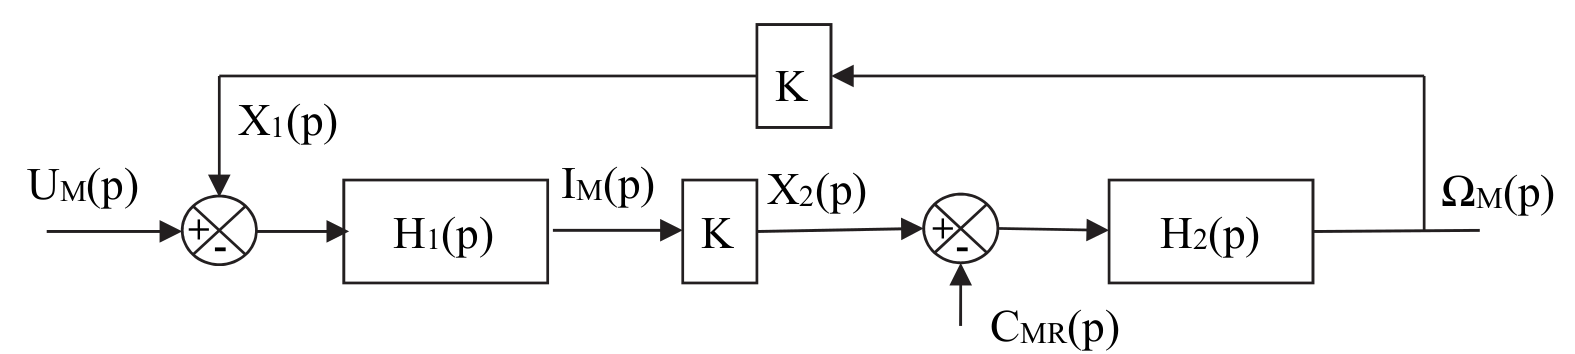
\includegraphics[width=0.8\linewidth]{img/fig21}
 \caption{Schéma bloc du moteur}
 \label{img21}
\end{figure}

\question{Donner le nom et l’unité des deux grandeurs physiques $x_1(t)$, $x_2(t)$ dont les transformées de Laplace sont notées respectivement $X_1(p)$, $X_2(p)$ (figure \ref{img21}).}

\question{À partir des équations de fonctionnement du M.C.C., retrouver l’expression des deux fonctions de transfert $H_1(p)$ et $H_2(p)$ (figure \ref{img21}).}

On néglige maintenant le couple résistant $C_{mr}(t)$ ainsi que l’inductance $L$ du moteur.

\question{Déterminer alors le schéma bloc simplifié ayant pour entrée $U_M(p)$ et pour sortie $\Omega_M(p)$.

En déduire la fonction de transfert $H(p)=\frac{\Omega_M(p)}{U_M(p)}$ et montrer qu'elle peut se mettre sous la forme $H(p)=\frac{K'}{1+\tau_m\cdot p}$. Exprimer alors $K'$ et $\tau_m$.}

\subsection{Étude du positionnement}

On souhaite d’abord étudier le positionnement de la tige du vérin.
Les performances attendues concernant la précision sont : écart par rapport à la consigne $< 1 mm$.

Un codeur incrémental à 2 voies en quadrature est placé sur l'axe de rotation moteur.

\question{Donner le principe de fonctionnement d’un tel codeur. Qualifier les signaux des deux voies du codeur en proposant un chronogramme.}

~\

On donne ci-dessous le schéma de principe d’un vérin électrique.

\begin{figure}[!h]
\centering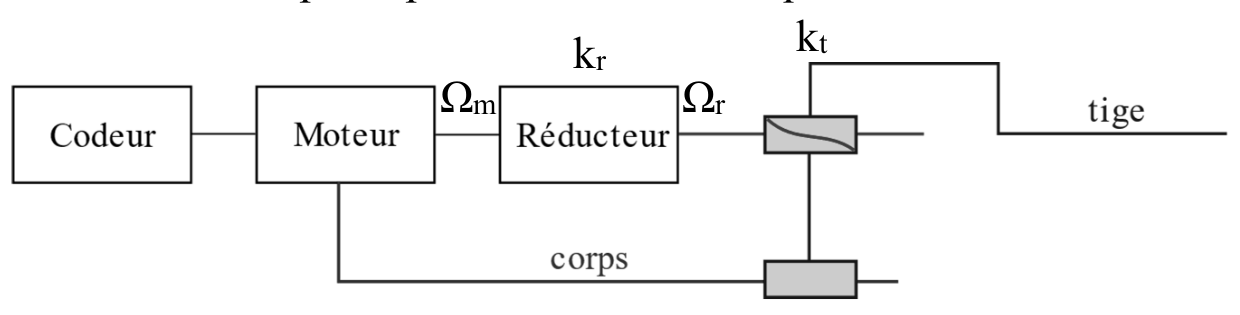
\includegraphics[width=0.7\linewidth]{img/fig22}
 \caption{Schéma de principe du schéma électrique}
 \label{img22}
\end{figure}

Avec $k_r=\frac{1}{3,5}$ (rapport de réduction du réducteur); $k_t=12,7 mm\cdot tr^{-1}$ (rapport de transmission écrou/vis).

\question{En vous aidant de la figure \ref{img22}, déterminer la résolution (nombre d'impulsions par tour) du codeur nécessaire pour obtenir une mesure du déplacement de la tige du vérin avec une précision minimale de 1 mm.}

~\

Le schéma bloc de l’asservissement en position est le suivant :
\begin{figure}[!h]
\centering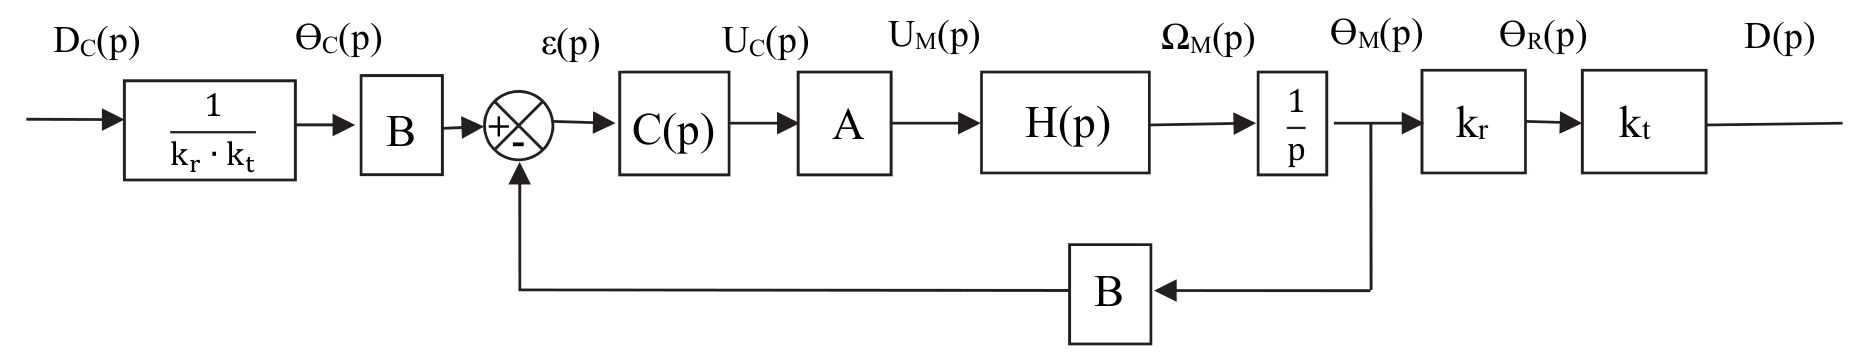
\includegraphics[width=0.9\linewidth]{img/fig24}
 \caption{Schéma bloc de la régulation de position}
 \label{img24}
\end{figure}

Avec:
\begin{itemize}
 \item $D_C$ : consigne de position [$mm$],
 \item $\theta_C$ : consigne d’angle demandée [$\degree\ $],
 \item $B$: gain de la chaîne de mesure de la position angulaire de l’arbre de sortie du moteur,
 \item $\varepsilon(p)$ : erreur,
 \item $C(p)$ : correcteur,
 \item $U_C(p)$ : tension de commande du variateur [$V$],
 \item $A$ : gain du variateur de commande du M.C.C.,
 \item $\Omega_M$ : vitesse de rotation de l’arbre de sortie du moteur [$\degree\cdot s^{-1}$],
 \item $\theta_M$ : angle de l’arbre de sortie du moteur [$\degree\ $],
 \item $k_r$ : rapport de réduction du réducteur,
 \item $\theta_R$ : angle de l’arbre de sortie du réducteur [$\degree\ $],
 \item $k_t$ : rapport de transmission vis/écrou [$mm\cdot tr^{-1}$],
 \item $D$ : position réelle de la tige du vérin [$mm$].
\end{itemize}

~\

On souhaite vérifier la nécessité de placer un correcteur et définir le réglage de celui-ci.

En première approche, le correcteur utilisé sera un correcteur proportionnel, tel que $C(p)=C$.

\question{Donner l’expression de B’ pour que le schéma bloc de l’asservissement puisse se mettre sous la forme du schéma bloc de la figure \ref{img25}. Proposer un schéma bloc équivalent avec un retour unitaire.}

\begin{figure}[!h]
\centering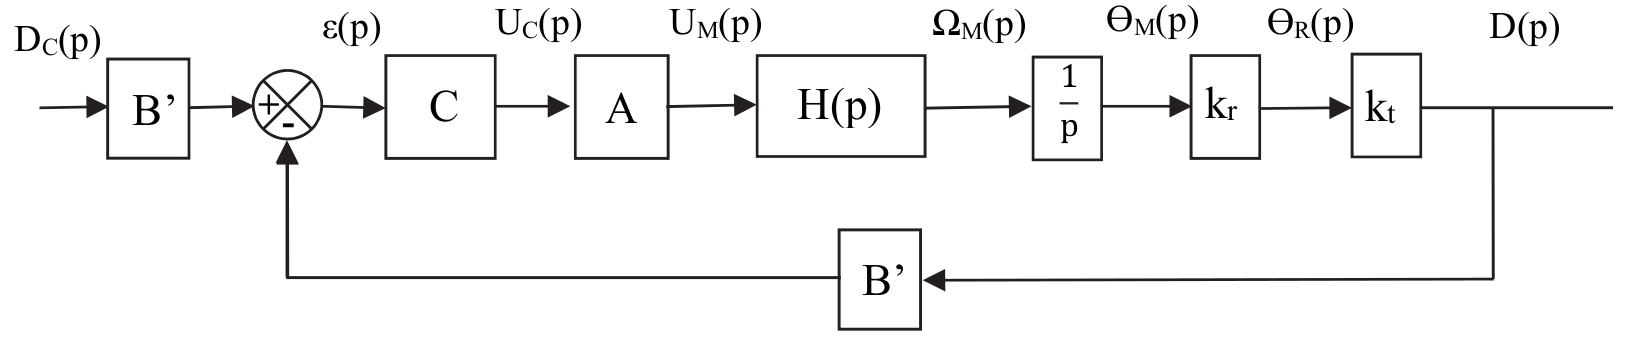
\includegraphics[width=0.75\linewidth]{img/fig25}
 \caption{Schéma bloc modifié de la régulation de position}
 \label{img25}
\end{figure}

\question{Déterminer alors la fonction de transfert en boucle ouverte, $G(p)$ (figure \ref{img26}) ; montrer qu’elle peut se mettre sous la forme : $G(p)=\frac{A_0}{(1+\tau_m\cdot p)\cdot p}$. Déterminer l'expression du gain $A_0$ en fonction de $A$, $B$ et $K'$.}

\begin{figure}[!h]
\centering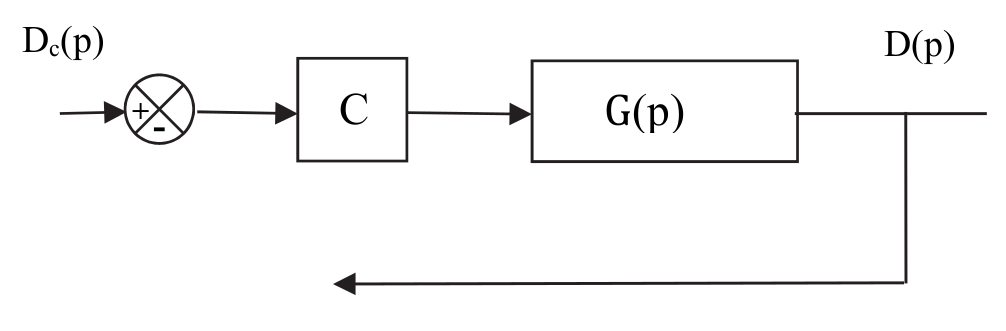
\includegraphics[width=0.45\linewidth]{img/fig26}
 \caption{Schéma bloc de la FTBO : $G(p)$}
 \label{img26}
\end{figure}

\question{Tracer l’allure des diagrammes asymptotiques de Bode (phase et gain) de la fonction de transfert $C\cdot G(p)$ sur le DR5.}

~\

Un essai indiciel, que vous trouverez sur le DR4, a été effectué sur le système décrit par la figure \ref{img27}. Cette schématisation est à relier avec la figure \ref{img24}.

\begin{figure}[!h]
\centering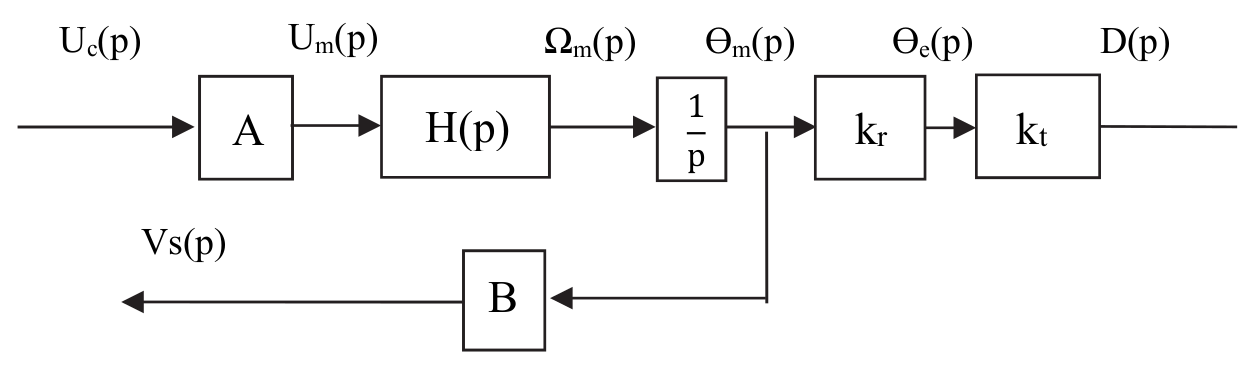
\includegraphics[width=0.55\linewidth]{img/fig27}
 \caption{Schéma bloc de l’essai indiciel}
 \label{img27}
\end{figure}

\newpage

Les courbes suivantes ont été relevées.

\begin{figure}[!h]
\centering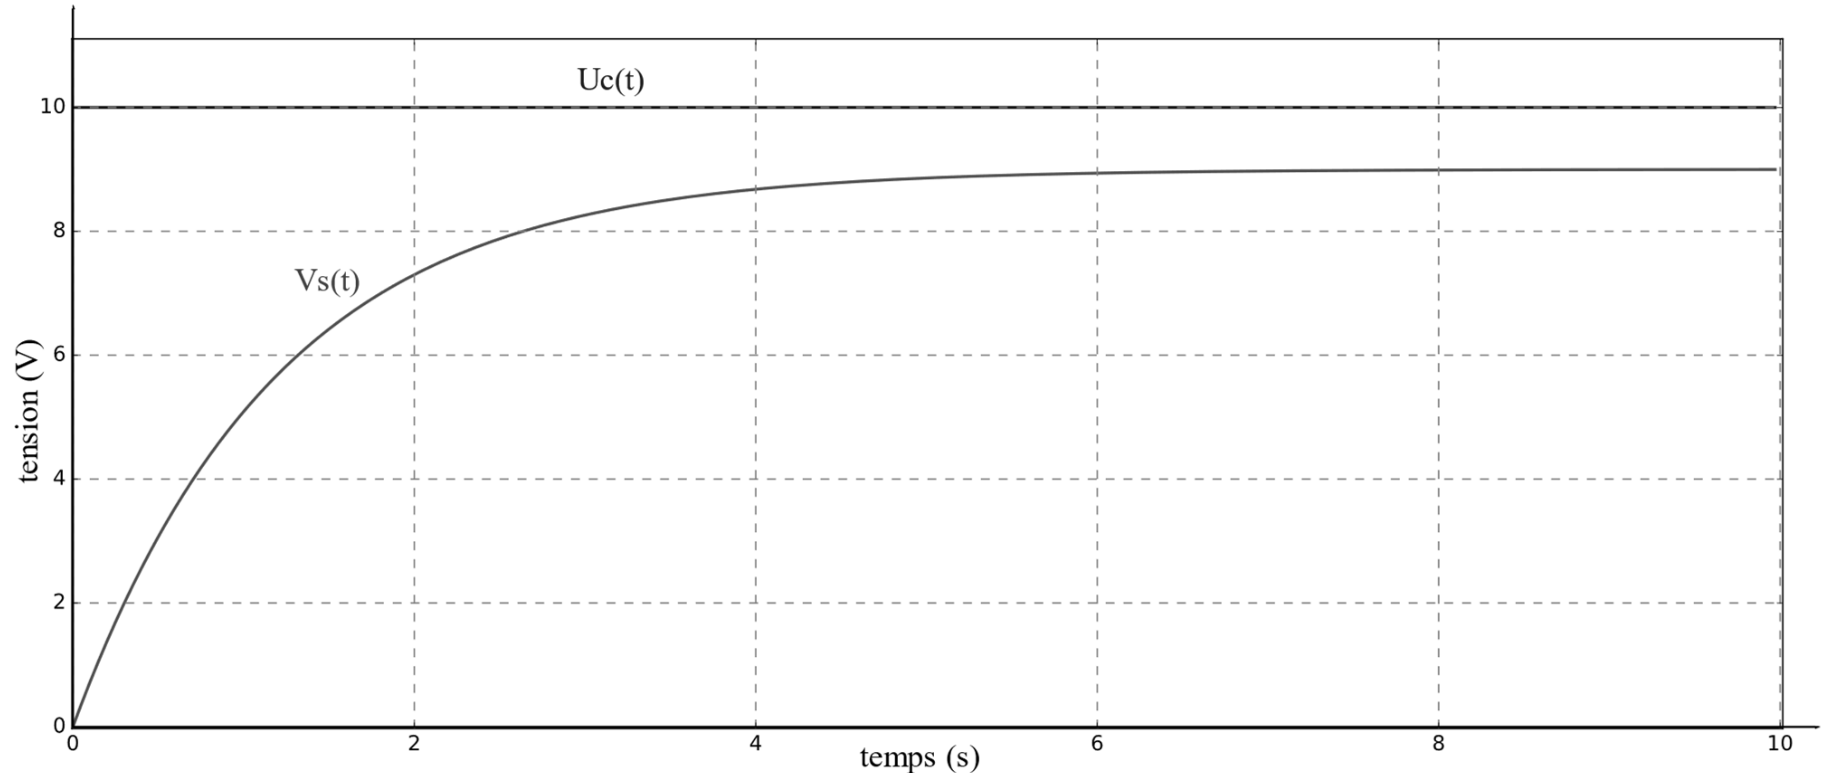
\includegraphics[width=\linewidth]{img/fig28}
 \caption{Consigne et réponse indicielle du système présenté à la figure \ref{img27}}
 \label{img28}
\end{figure}

\question{Déduire graphiquement, à partir du DR4, la constante de temps $\tau_m$ et le gain $A_0$ définis à la question Q33. Indiquer sur le DR4 les grandeurs utiles.}

\subsection{Commande du moteur à courant continu du vérin}

On utilise la structure suivante pour commander le M.C.C.

\begin{figure}[!h]
\centering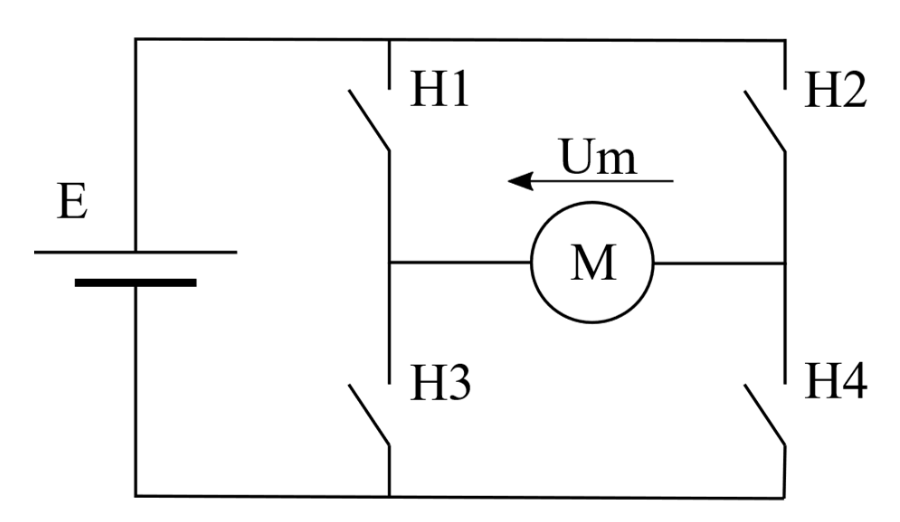
\includegraphics[width=0.5\linewidth]{img/fig30}
 \caption{Schéma de principe de commande du M.C.C.}
 \label{img30}
\end{figure}

\question{Dans quels quadrants de fonctionnement, dans le plan couple-vitesse, le moteur M.C.C. doit-il pouvoir fonctionner ? Justifier votre réponse.

Donner le nom du convertisseur statique de la figure \ref{img30}.}

\question{Proposer un chronogramme de commande des interrupteurs H1, H2, H3 et H4 permettant de faire varier la vitesse du moteur, dans le cas où le berceau monte (Um > 0).

Préciser le type d’interrupteurs à utiliser pour permettre ce fonctionnement.}

\begin{center}
\Large{--- Fin du sujet ---}
\end{center}

\includepdf[offset=0mm -10mm,pages={23-25,27}]{img/sciences_industrielles_TSI7SI.pdf}

\cleardoublepage

\ifdef{\public}{\pagestyle{documentreponse}}{\pagestyle{correction}}

\reponse{0}{\begin{center}
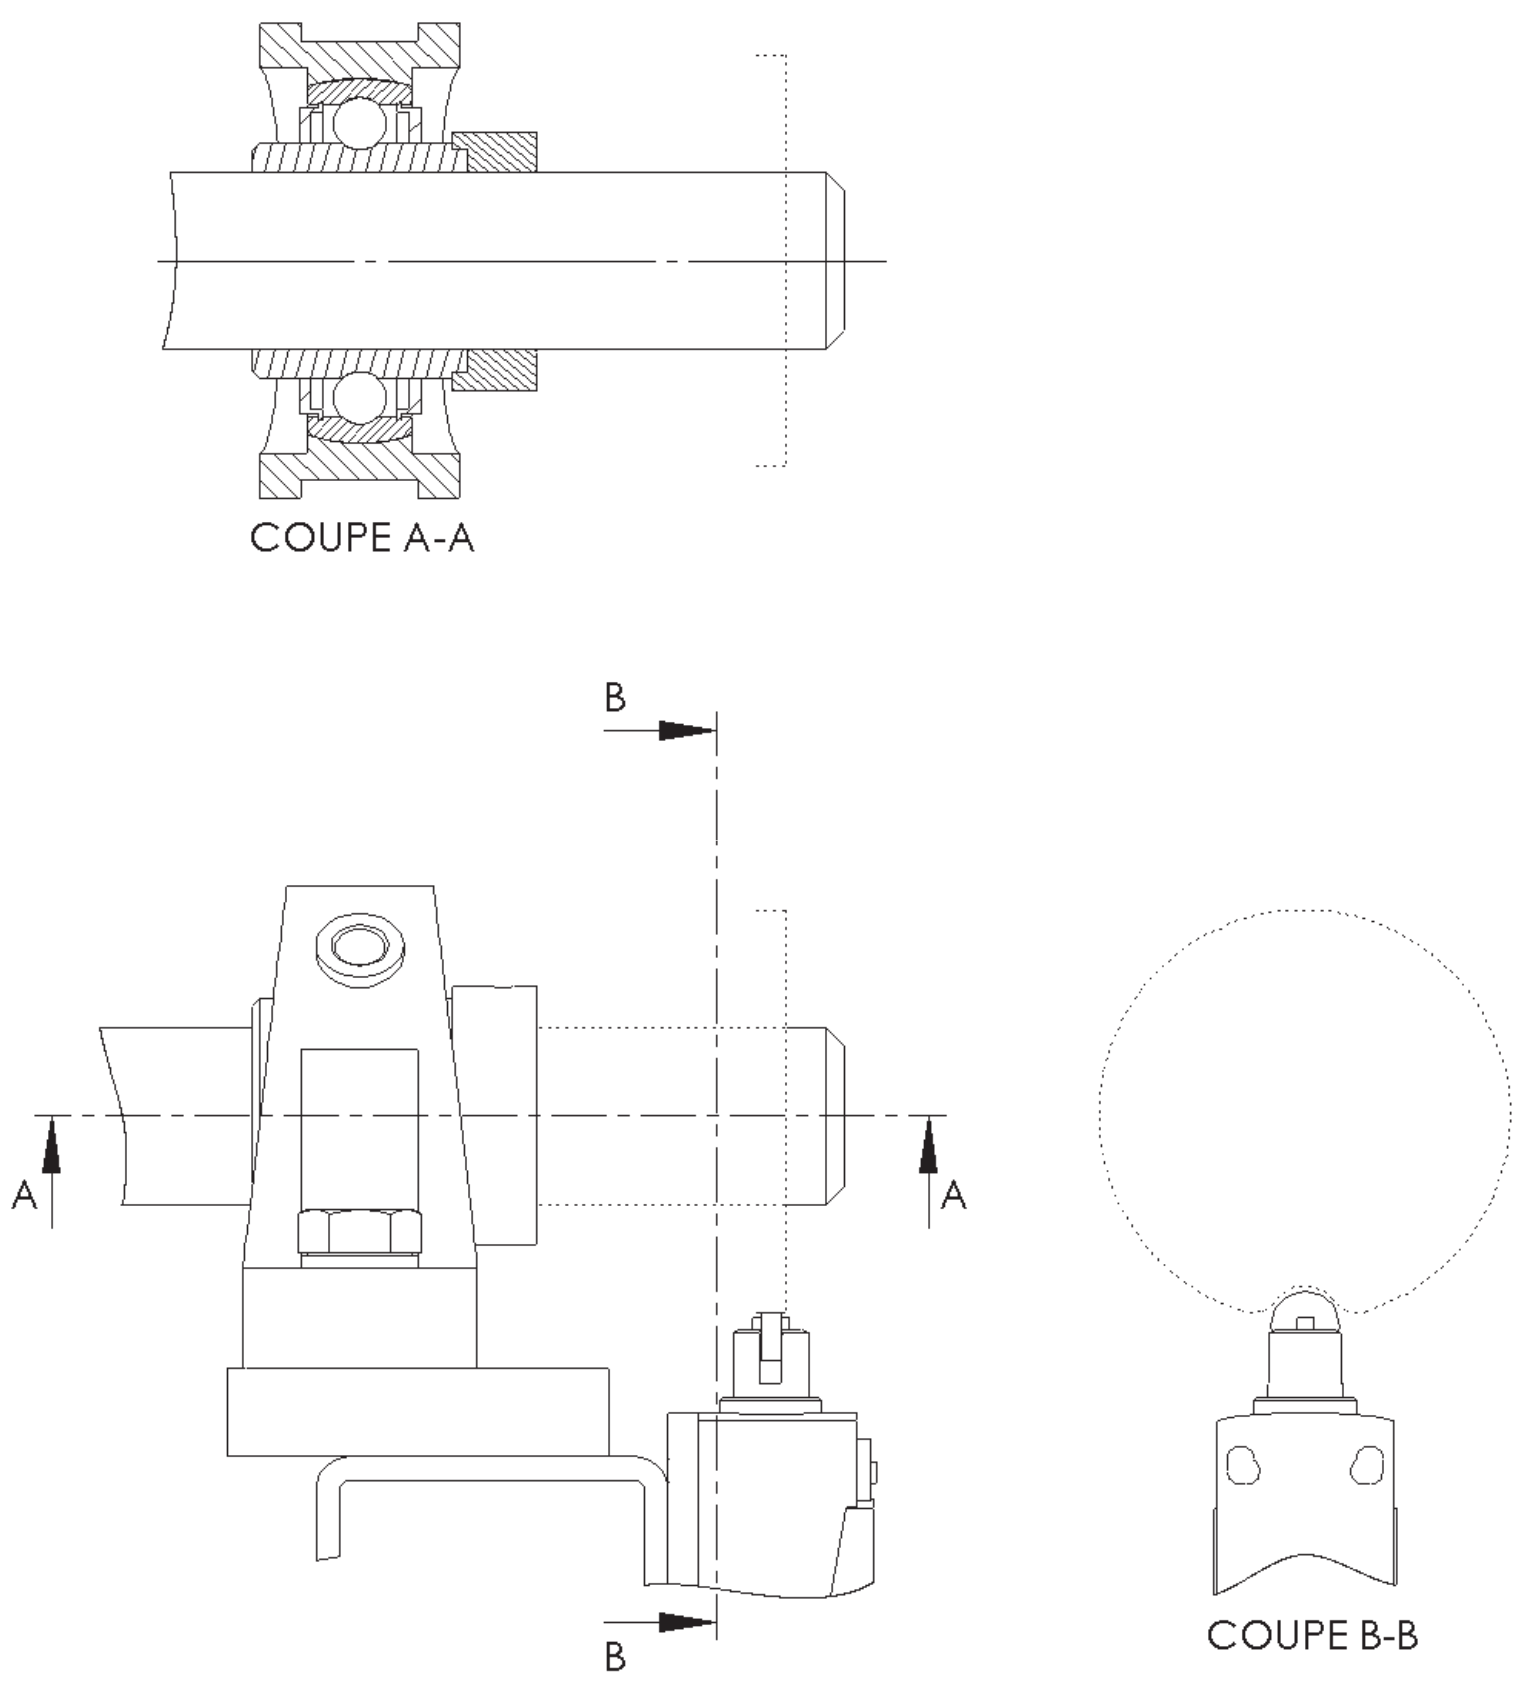
\includegraphics[width=\linewidth]{img/DR01}
\end{center}}{\begin{center}
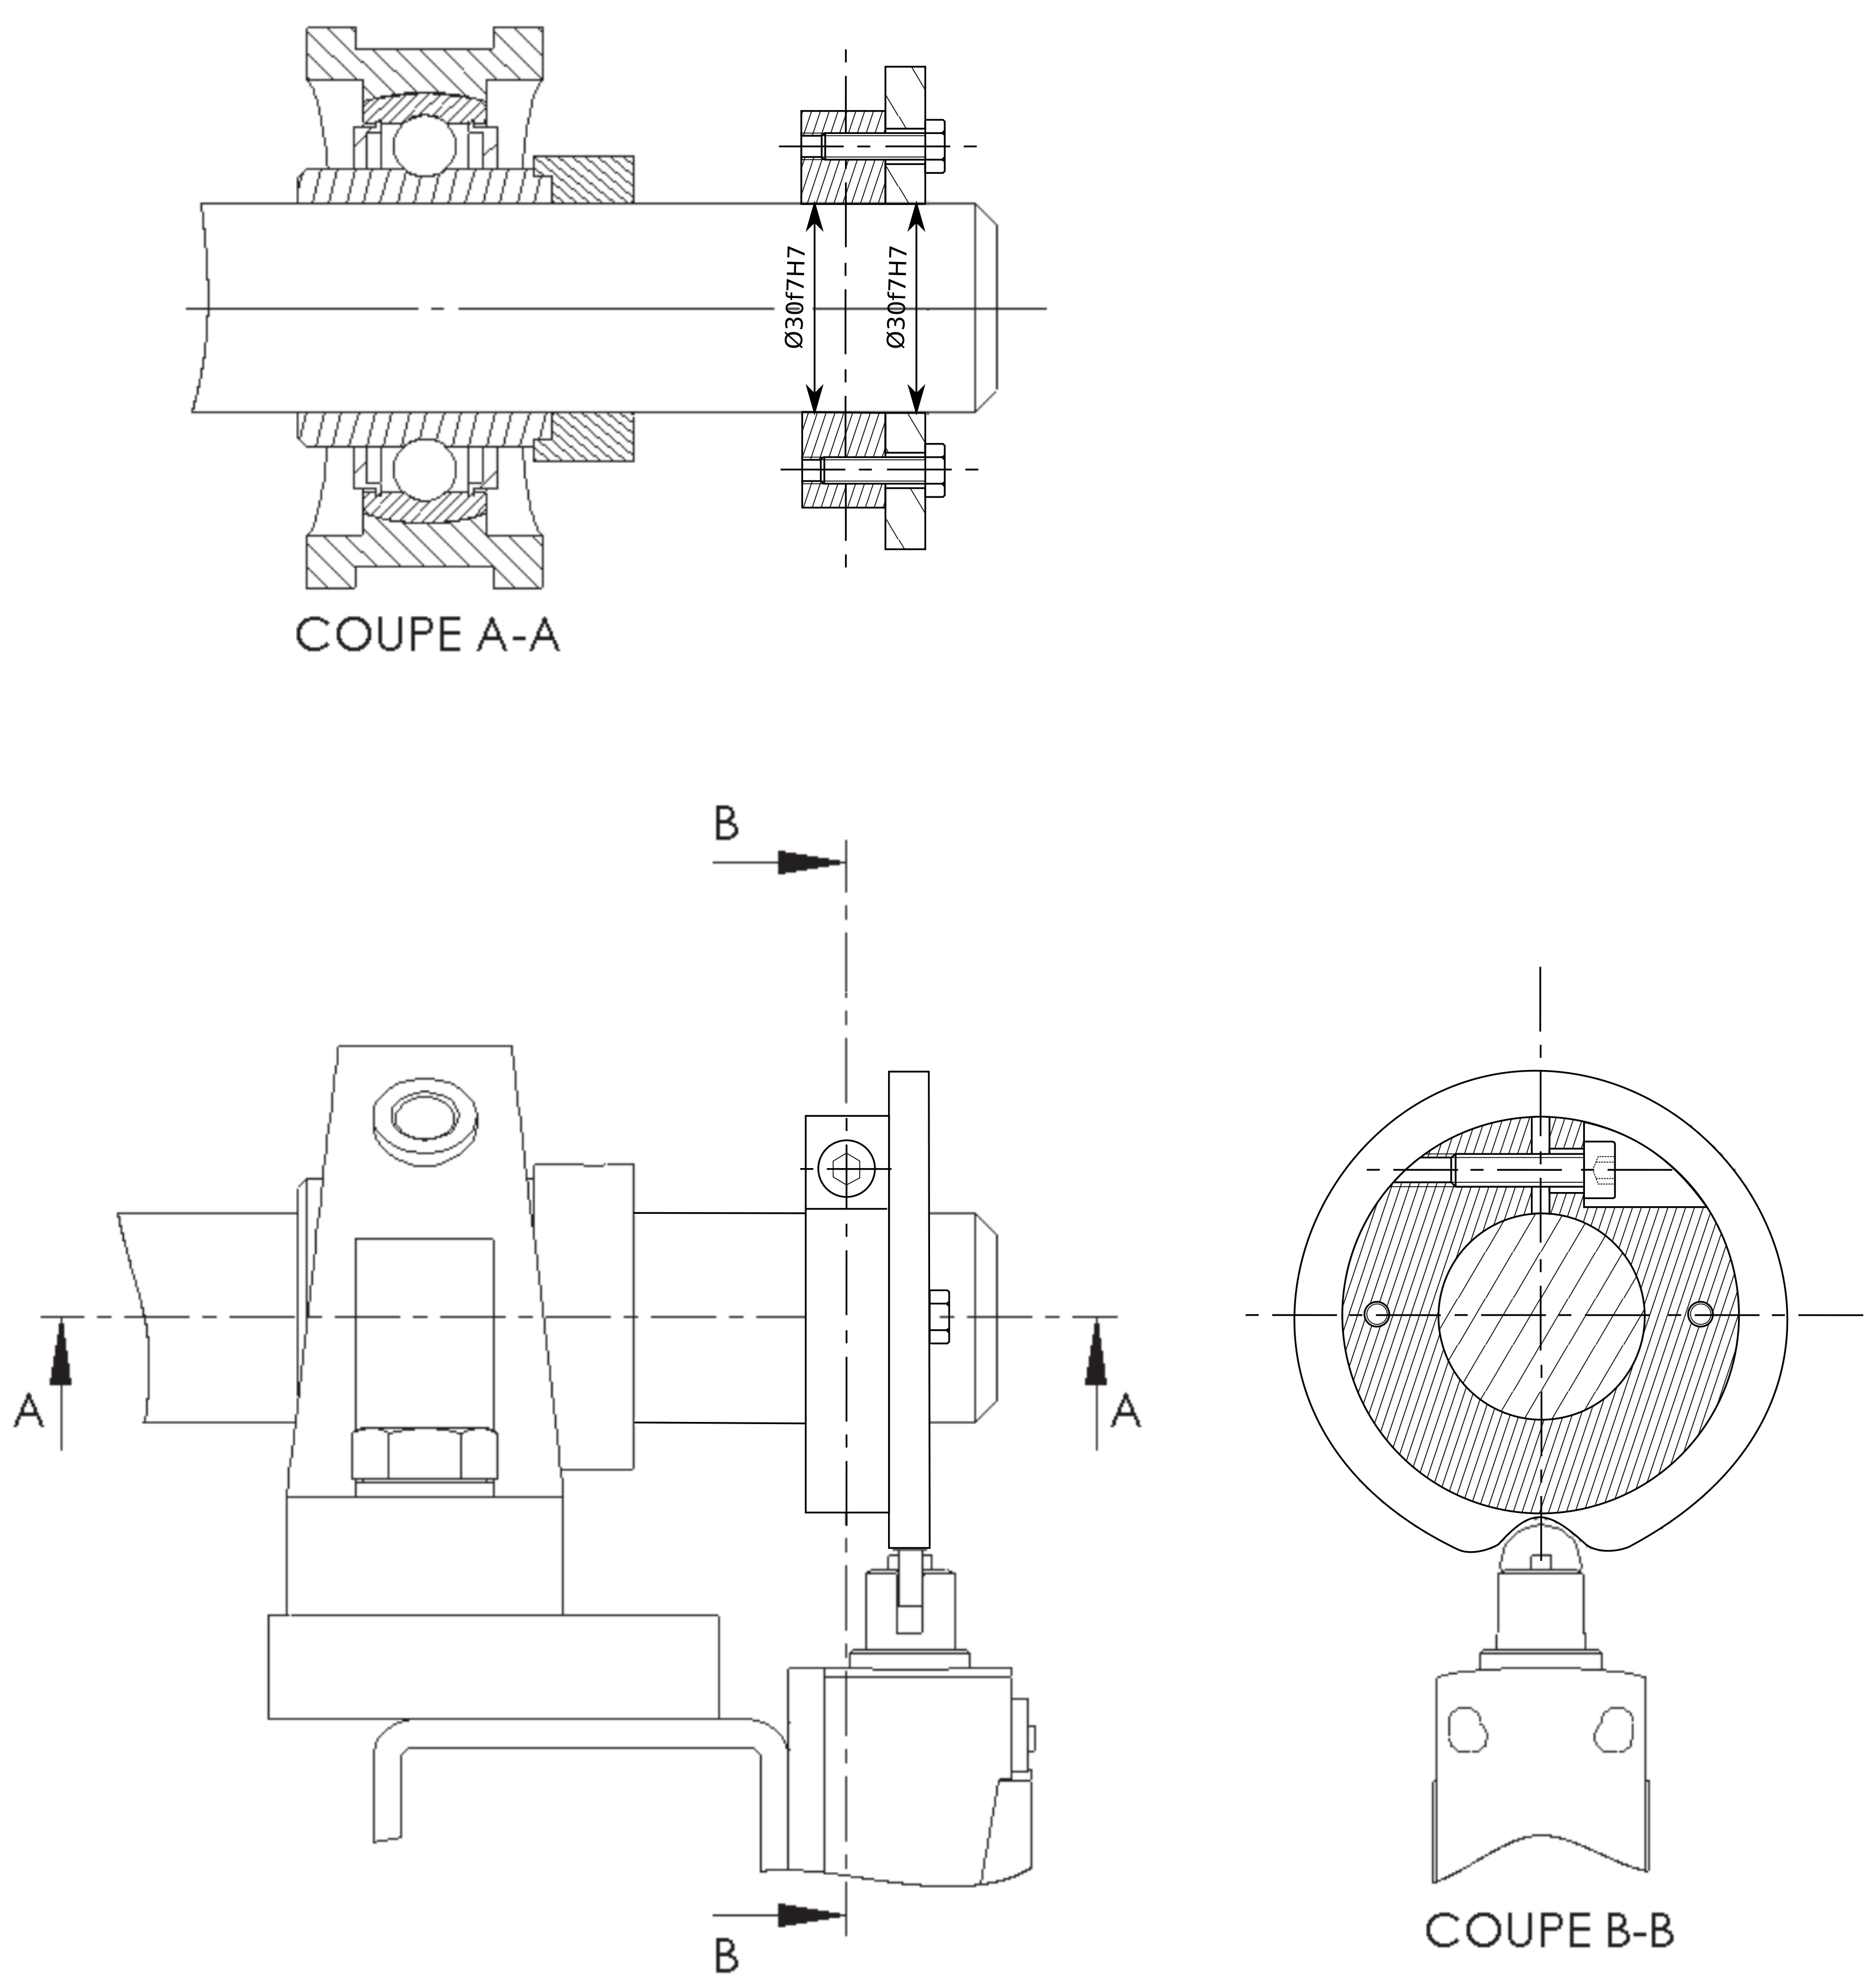
\includegraphics[width=\linewidth]{img/DR01_cor}
\end{center}
}

\reponse{0}{Réponse sur le document de la question 1.}{Réponse sur le document de la question 1.}

\reponse{2}{}{Le centre de gravité doit être sur l’axe de la rotation.}

\reponse{7}{}{
  On a donc:
  \[X_{GT} = \frac{M_{A}X_{A} - M_{G}X_{G}}{M_{A} + M_{G}}\] et
  \[Y_{GT} = -\frac{M_{A}Y_{A} + M_{G}{(Y_{A} - Y}_{GA})}{M_{A} + M_{G}}\]

  GT doit être positionné sur l'axe de rotation donc
  \[X_{GT} = 0\] et \[Y_{GT} = 0\].

  Enfin \[M_{A}X_{A} - M_{G}X_{G} = 0\] et
  \[M_{A}Y_{A} + M_{G}{(Y_{A} - Y}_{GA}) = 0\]
}

\reponse{3}{}{
  On déduit \[M_{A} = \frac{M_{G}}{X_{A}}X_{G}\] et
  \[Y_{A} = \frac{X_{A}}{X_{A} + X_{G}}Y_{GA}\]
}

\reponse{3}{}{
  \[M_{GT} = M_{A} + M_{G}\]
  \[Z_{GT} = \frac{M_{A}Z_{A} + M_{G}Z_{G}}{M_{A} + M_{G}} = \frac{M_{G}}{M_{A} + M_{G}}Z_{G}\]
  \[G_{T}(0;0;\frac{M_{G}}{M_{A} + M_{G}}Z_{G})\]
}

\reponse{3}{}{
  \[\overrightarrow{OE} + \overrightarrow{ED} + \overrightarrow{DC} + \overrightarrow{CO} = \overrightarrow{0}\]
  et donc
  \[\lambda\overrightarrow{y_{0}} + \ l_{2}\ \overrightarrow{y_{2}} - l_{3}\ \overrightarrow{x_{3}} - l_{x}\ \overrightarrow{x_{0}} - l_{y}\ \overrightarrow{y_{0}} = \ \overrightarrow{0}\]
}

\reponse{4}{}{
 \[\lambda\overrightarrow{y_{0}} + \ l_{2}(\cos\alpha\ \overrightarrow{y_{0}} - \sin\alpha\overrightarrow{x_{0}}) - l_{3}\ (\cos\beta\ \overrightarrow{x_{0}} + \sin\beta\overrightarrow{y_{0}}) - l_{x}\ \overrightarrow{x_{0}} - l_{y}\ \overrightarrow{y_{0}} = \ \overrightarrow{0}\]

\begin{eqnarray}
-{l_{2}\sin}\alpha - l_{3}\ \cos\beta - l_{x} = 0\\
\lambda + l_{2}\cos\alpha\  - l_{3}\ \sin\beta - l_{y}\  = \ 0
\end{eqnarray}
}

\reponse{4}{}{

D'après la question précédente:
\begin{eqnarray}
-{l_{2}\sin}\alpha = l_{3}\ \cos\beta + l_{x}\\
l_{2}\cos\alpha\  = l_{3}\ \sin\beta + l_{y}\  -\lambda
\end{eqnarray}

\[l_{2}^{2} = l_{3}^{2}\cos^{2}\beta + 2l_{x}l_{3}\cos\beta + l_{x}^{2} + l_{3}^{2}\sin^{2}\beta + 2l_{3}\left( l_{y} - \lambda \right)\sin\beta + l_{y}^{2} - 2l_{y}\lambda + \lambda^{2}\ \]

  \[l_{2}^{2} = l_{3}^{2} + 2l_{x}l_{3}\cos\beta + 2l_{3}\left( l_{y} - \lambda \right)\sin\beta + l_{x}^{2} + l_{y}^{2} - 2l_{y}\lambda + \lambda^{2}\]
}

\reponse{5}{}{

La pièce \textbf{2} est soumise à 2 actions mécaniques extérieures (pivot en D et E). Elles sont donc de même direction $\overrightarrow{x_{0}}$ mais de sens opposé.

L'ensemble \{1+2\} est soumis à 3 actions mécaniques (en D, F et O). On vient de montrer que l'action en D est de direction $\overrightarrow{x_{0}}$ et n'a pas de composante selon
  $\overrightarrow{y_{0}}$). La liaison glissière en O n'a pas de composante selon $\overrightarrow{y_{0}}$, donc $Y_{F} = 0$.
}

\reponse{2}{}{
C'est un distributeur 5/3 bistable, sa commande est manuelle ou pneumatique ou électronique, elle est monostable de par la présence des ressorts.
}

\reponse{0}{\begin{center}
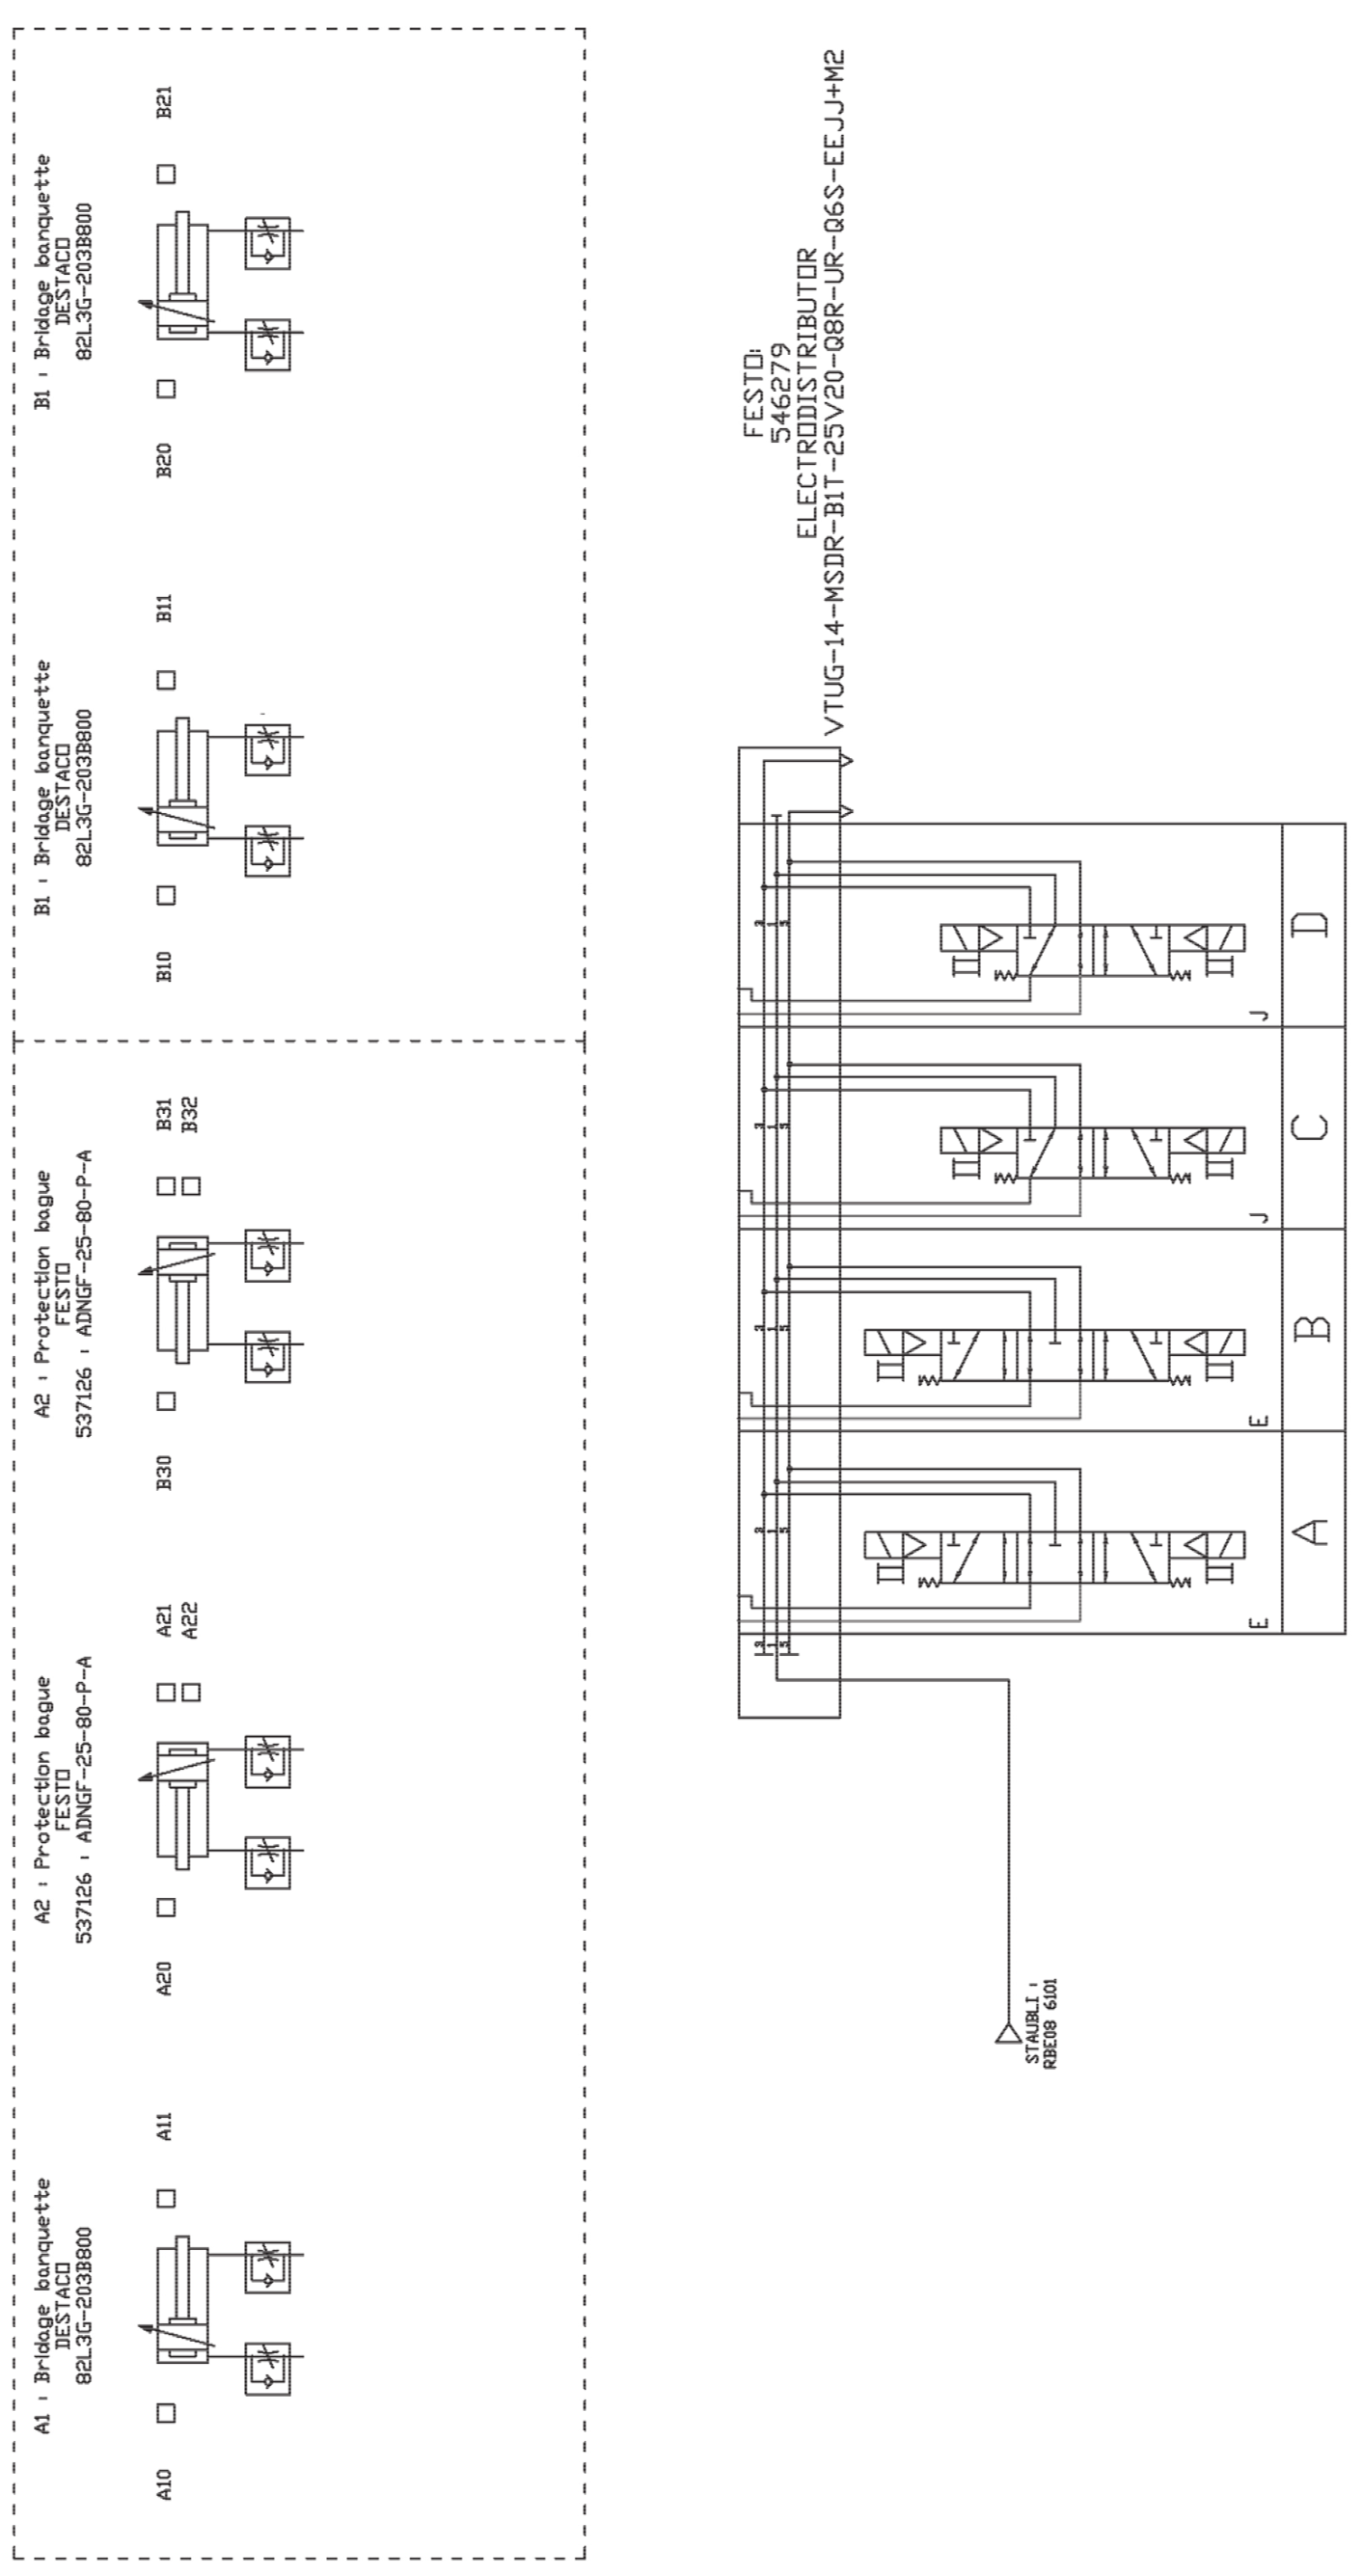
\includegraphics[width=0.6\linewidth]{img/DR02}
\end{center}}{\begin{center}
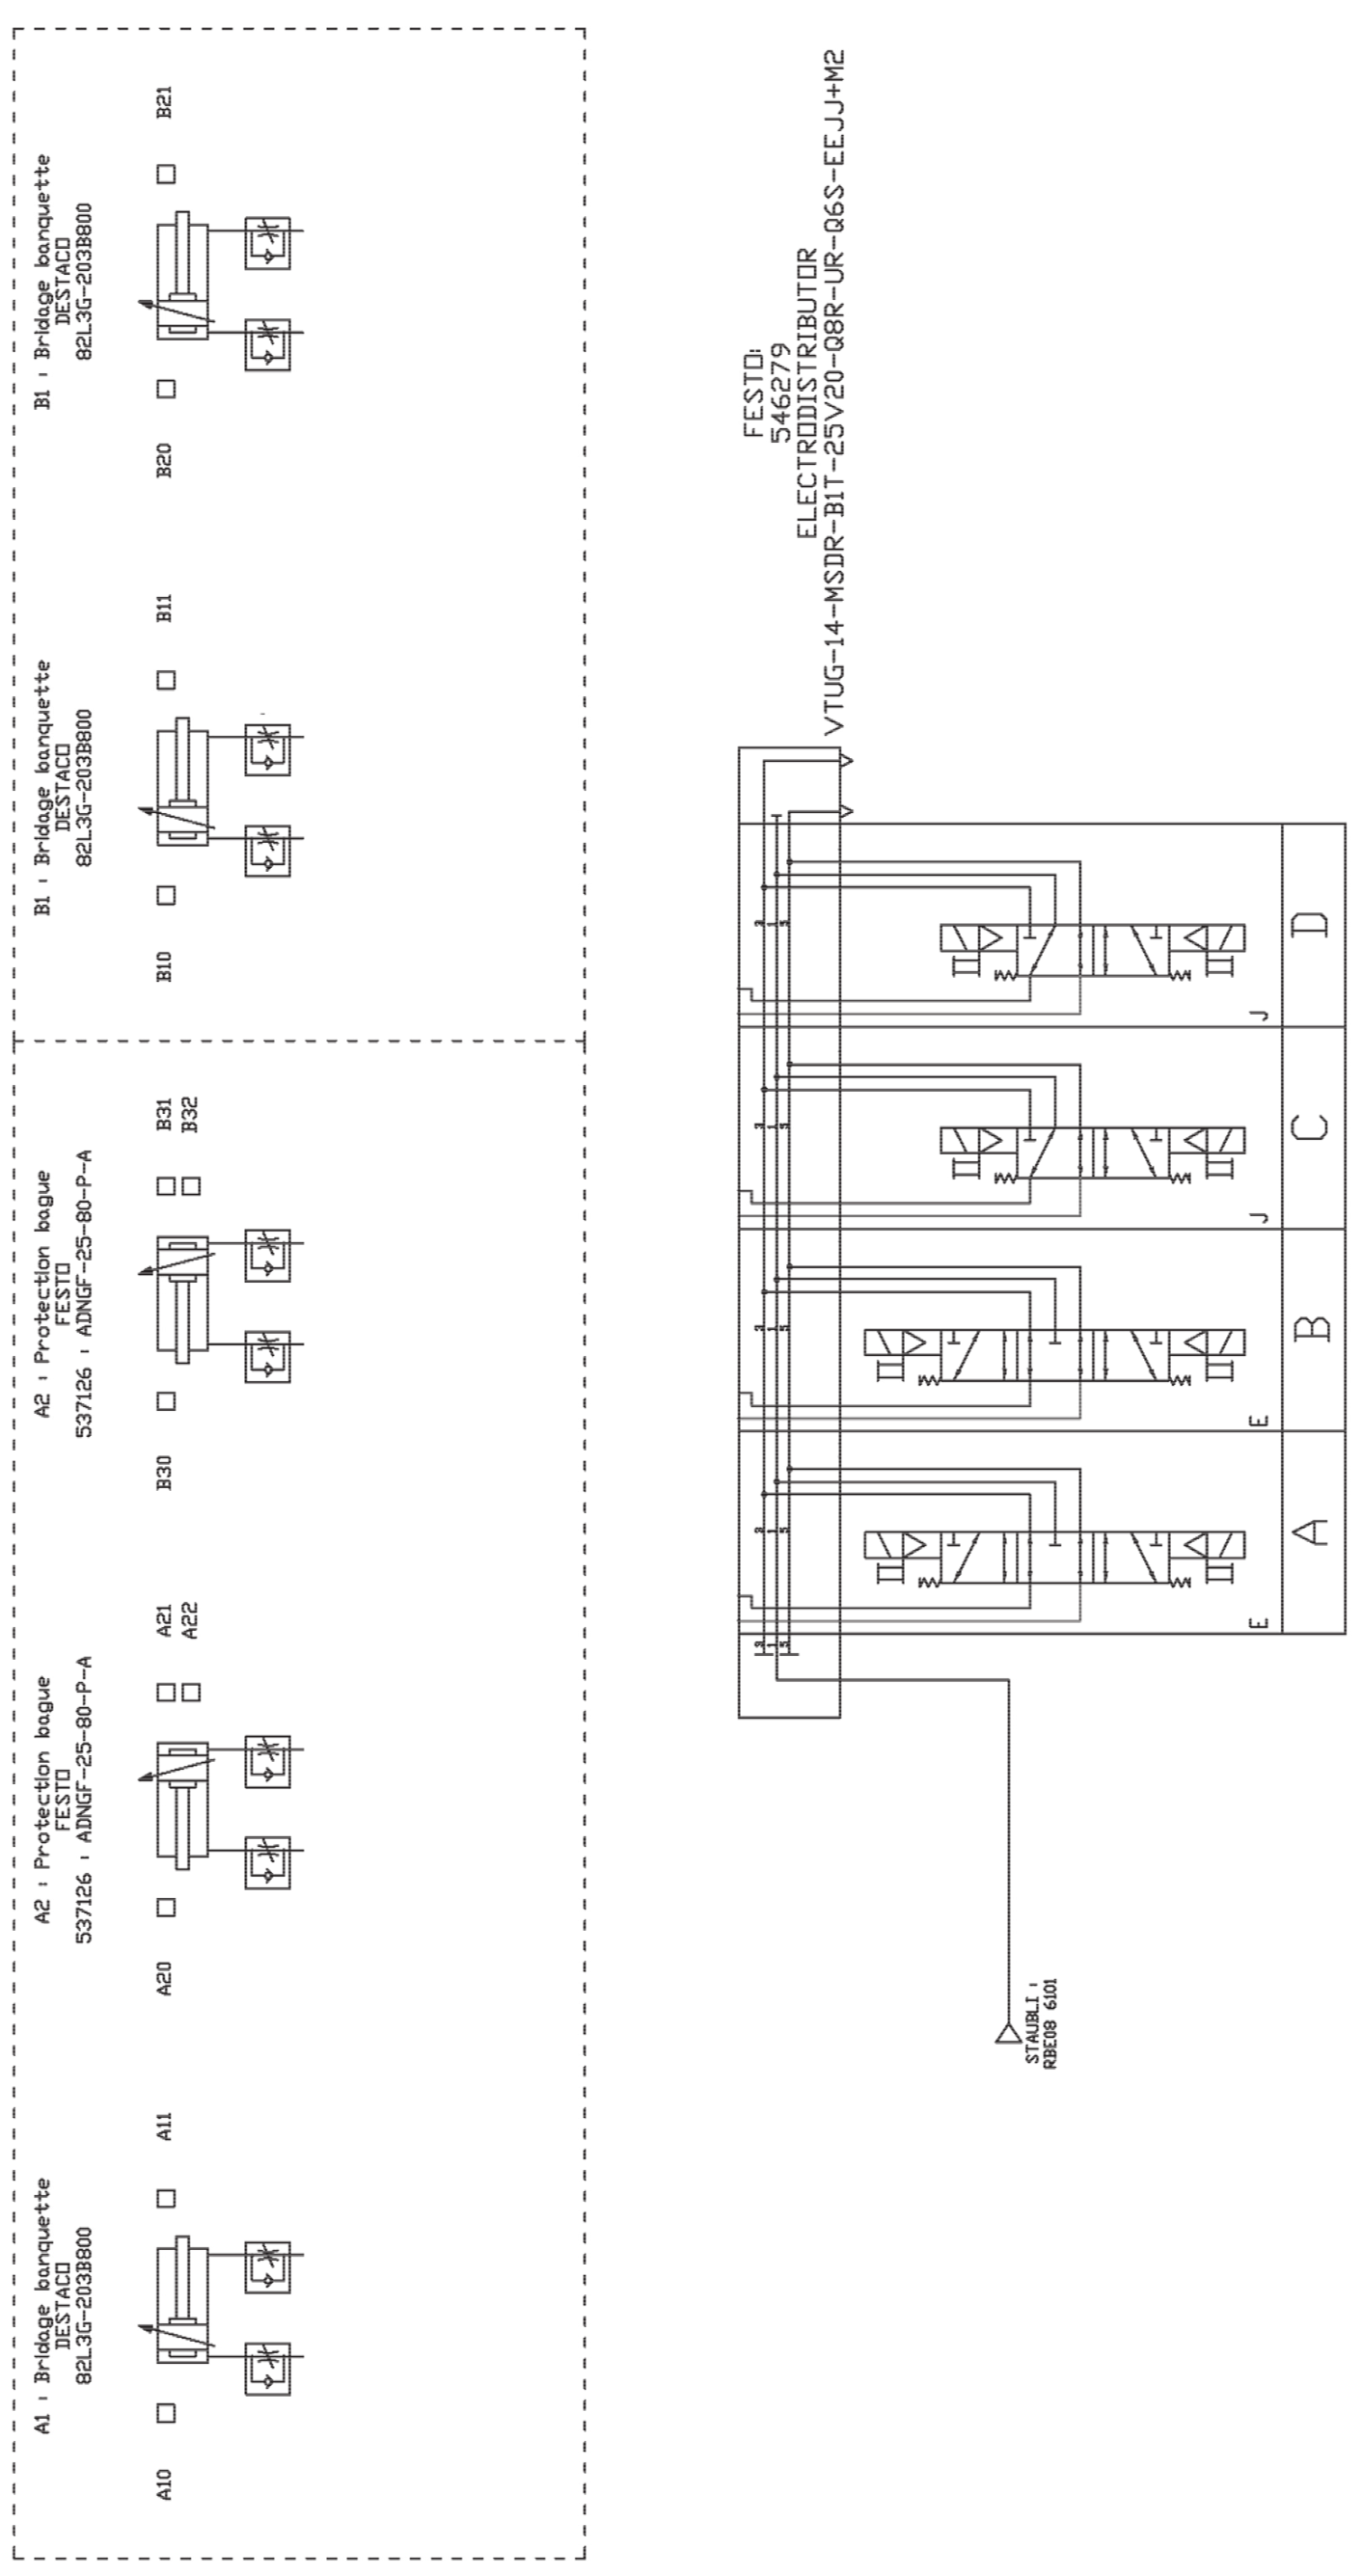
\includegraphics[width=0.6\linewidth]{img/DR02}
\end{center}
}

\reponse{5}{}{
Le transformateur permet d'abaisser la tension de 380 V à 230V. 
Un gradateur, ou l'association d'un redresseur, d'un hacheur et d'un onduleur serait d'autres solution possibles mais elles ont un moins bon rendement.
}

\reponse{8}{}{
\begin{itemize}
 \item Prise coffret~: 230 x 6 = 1380 VA\tabularnewline
 \item Ventilateur coffret~: 12.5 VA\tabularnewline
 \item Prise machine~: 10 x 230 = 2300 VA\tabularnewline
 \item Ventilateur opérateur~: 6 x 230 = 1380 VA\tabularnewline
 \item Éclairage~: 4 x 18 = 72 VA\tabularnewline
 \item Commande vérins~: 2 x 215 = 430 VA\tabularnewline
 \item Alimentation 24V~: 24 x 5 = 120 VA\tabularnewline
\end{itemize}

Ce qui fait un total de 5694.5 VA, en ajoutant une majoration de 20\%(1139 VA), cela fait un total de 6833.5 VA.
}

\ifdef{\public}{\newpage}

\reponse{0}{\begin{center}
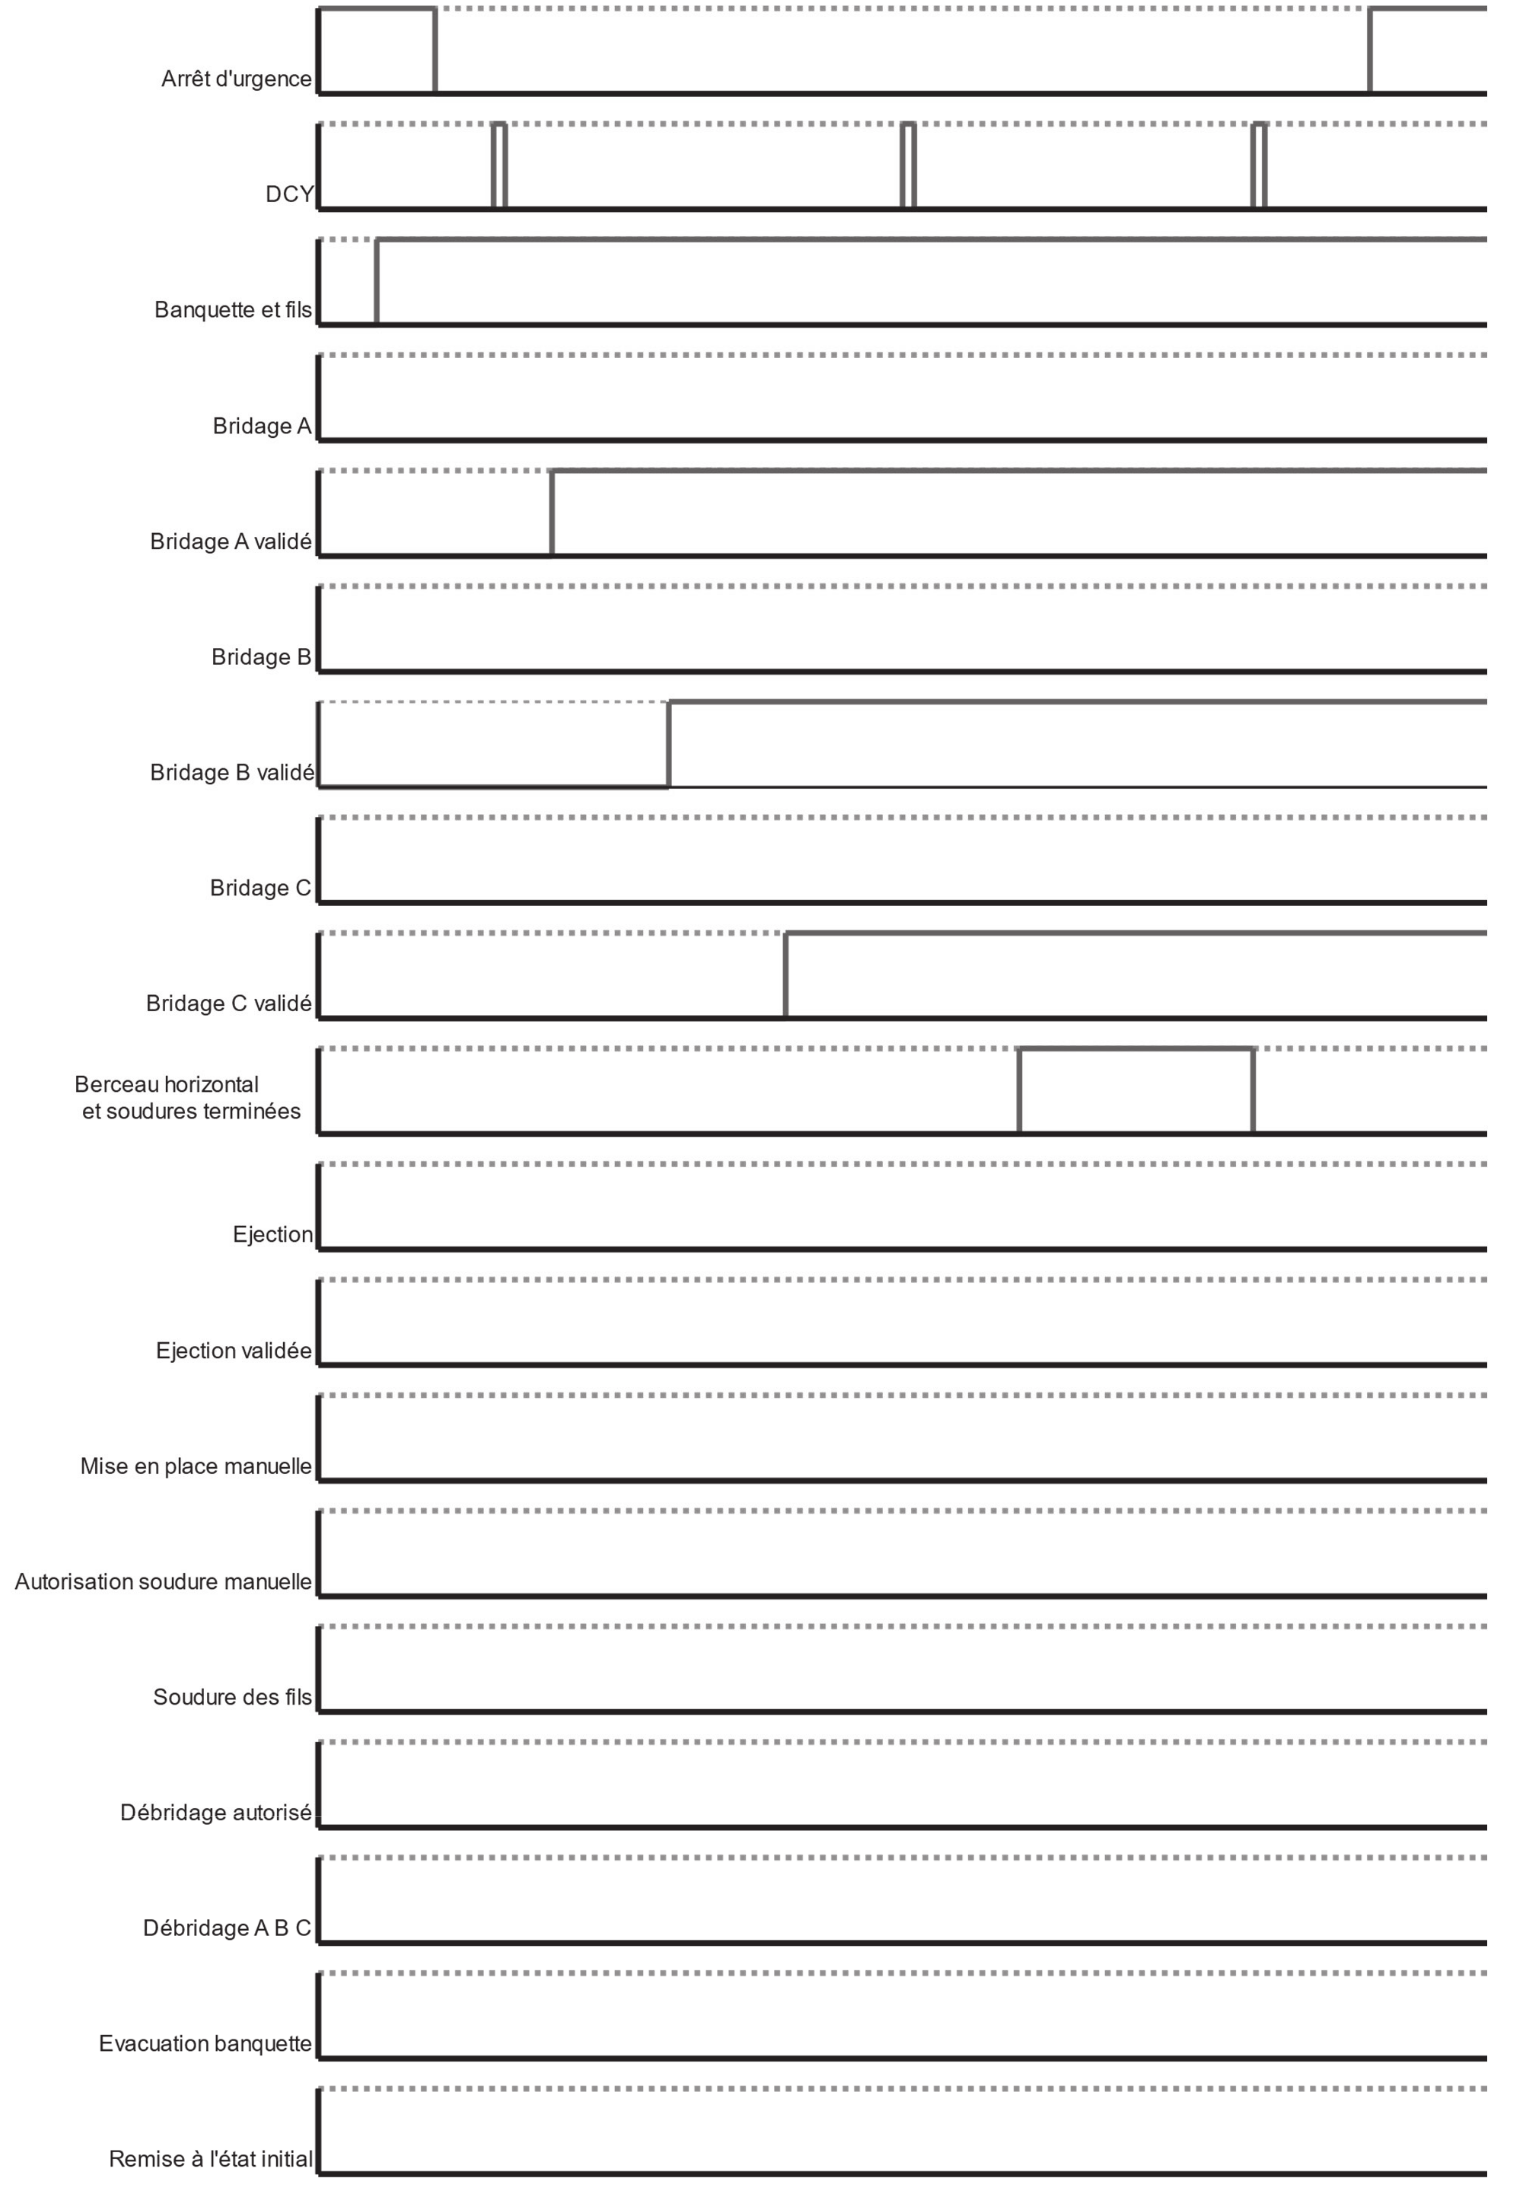
\includegraphics[width=0.9\linewidth]{img/DR03}
\end{center}}{\begin{center}
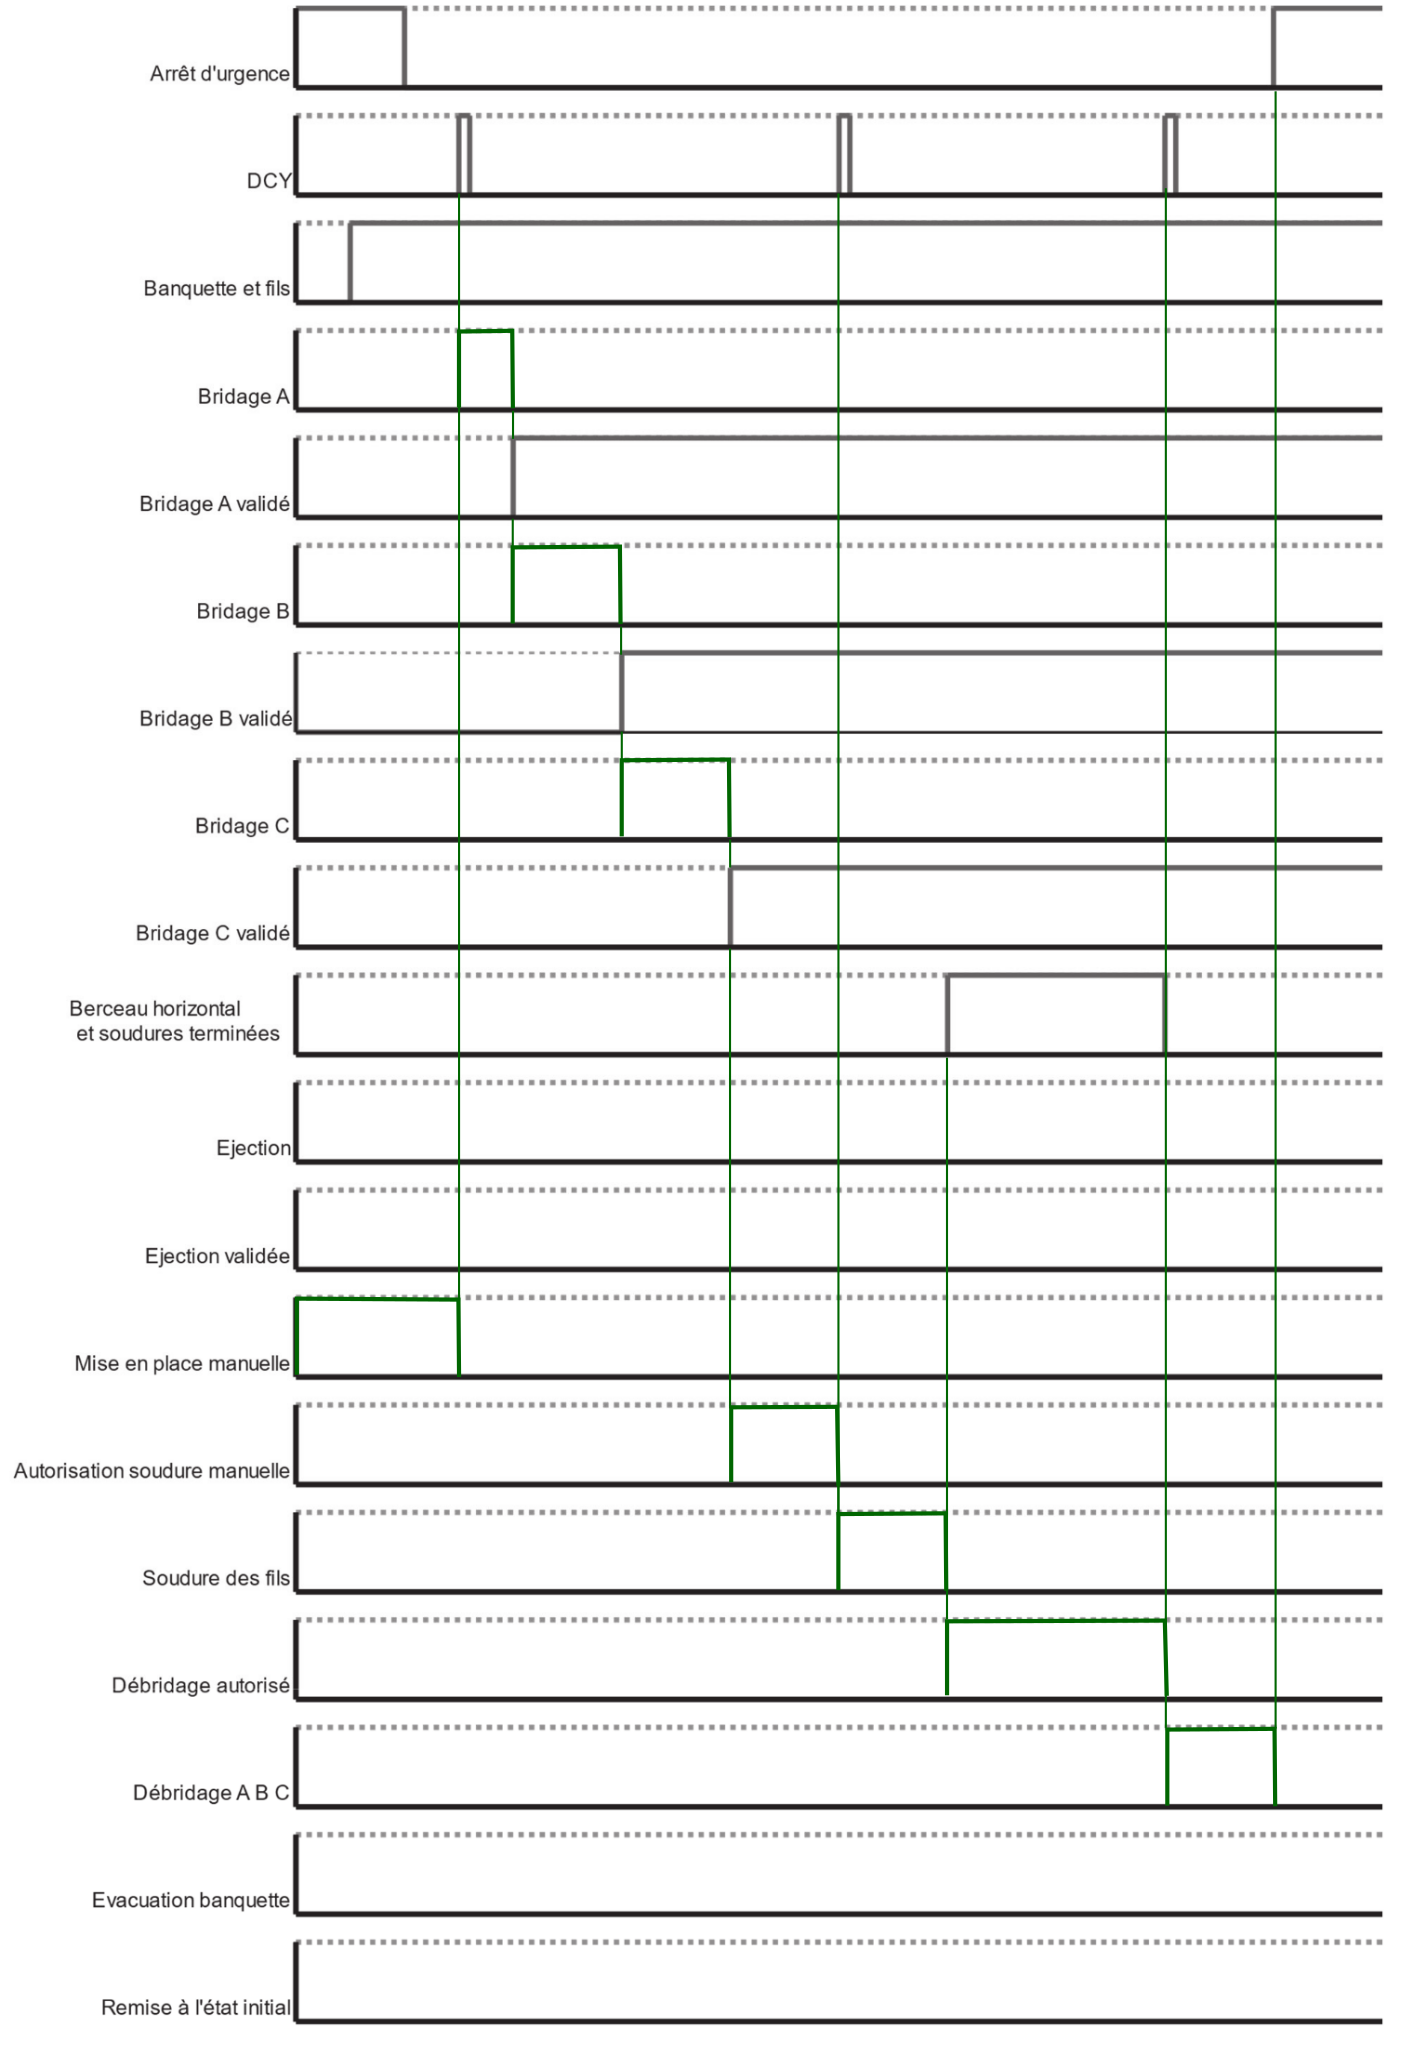
\includegraphics[width=0.9\linewidth]{img/DR03_cor}
\end{center}
}

\reponse{0}{\begin{center}
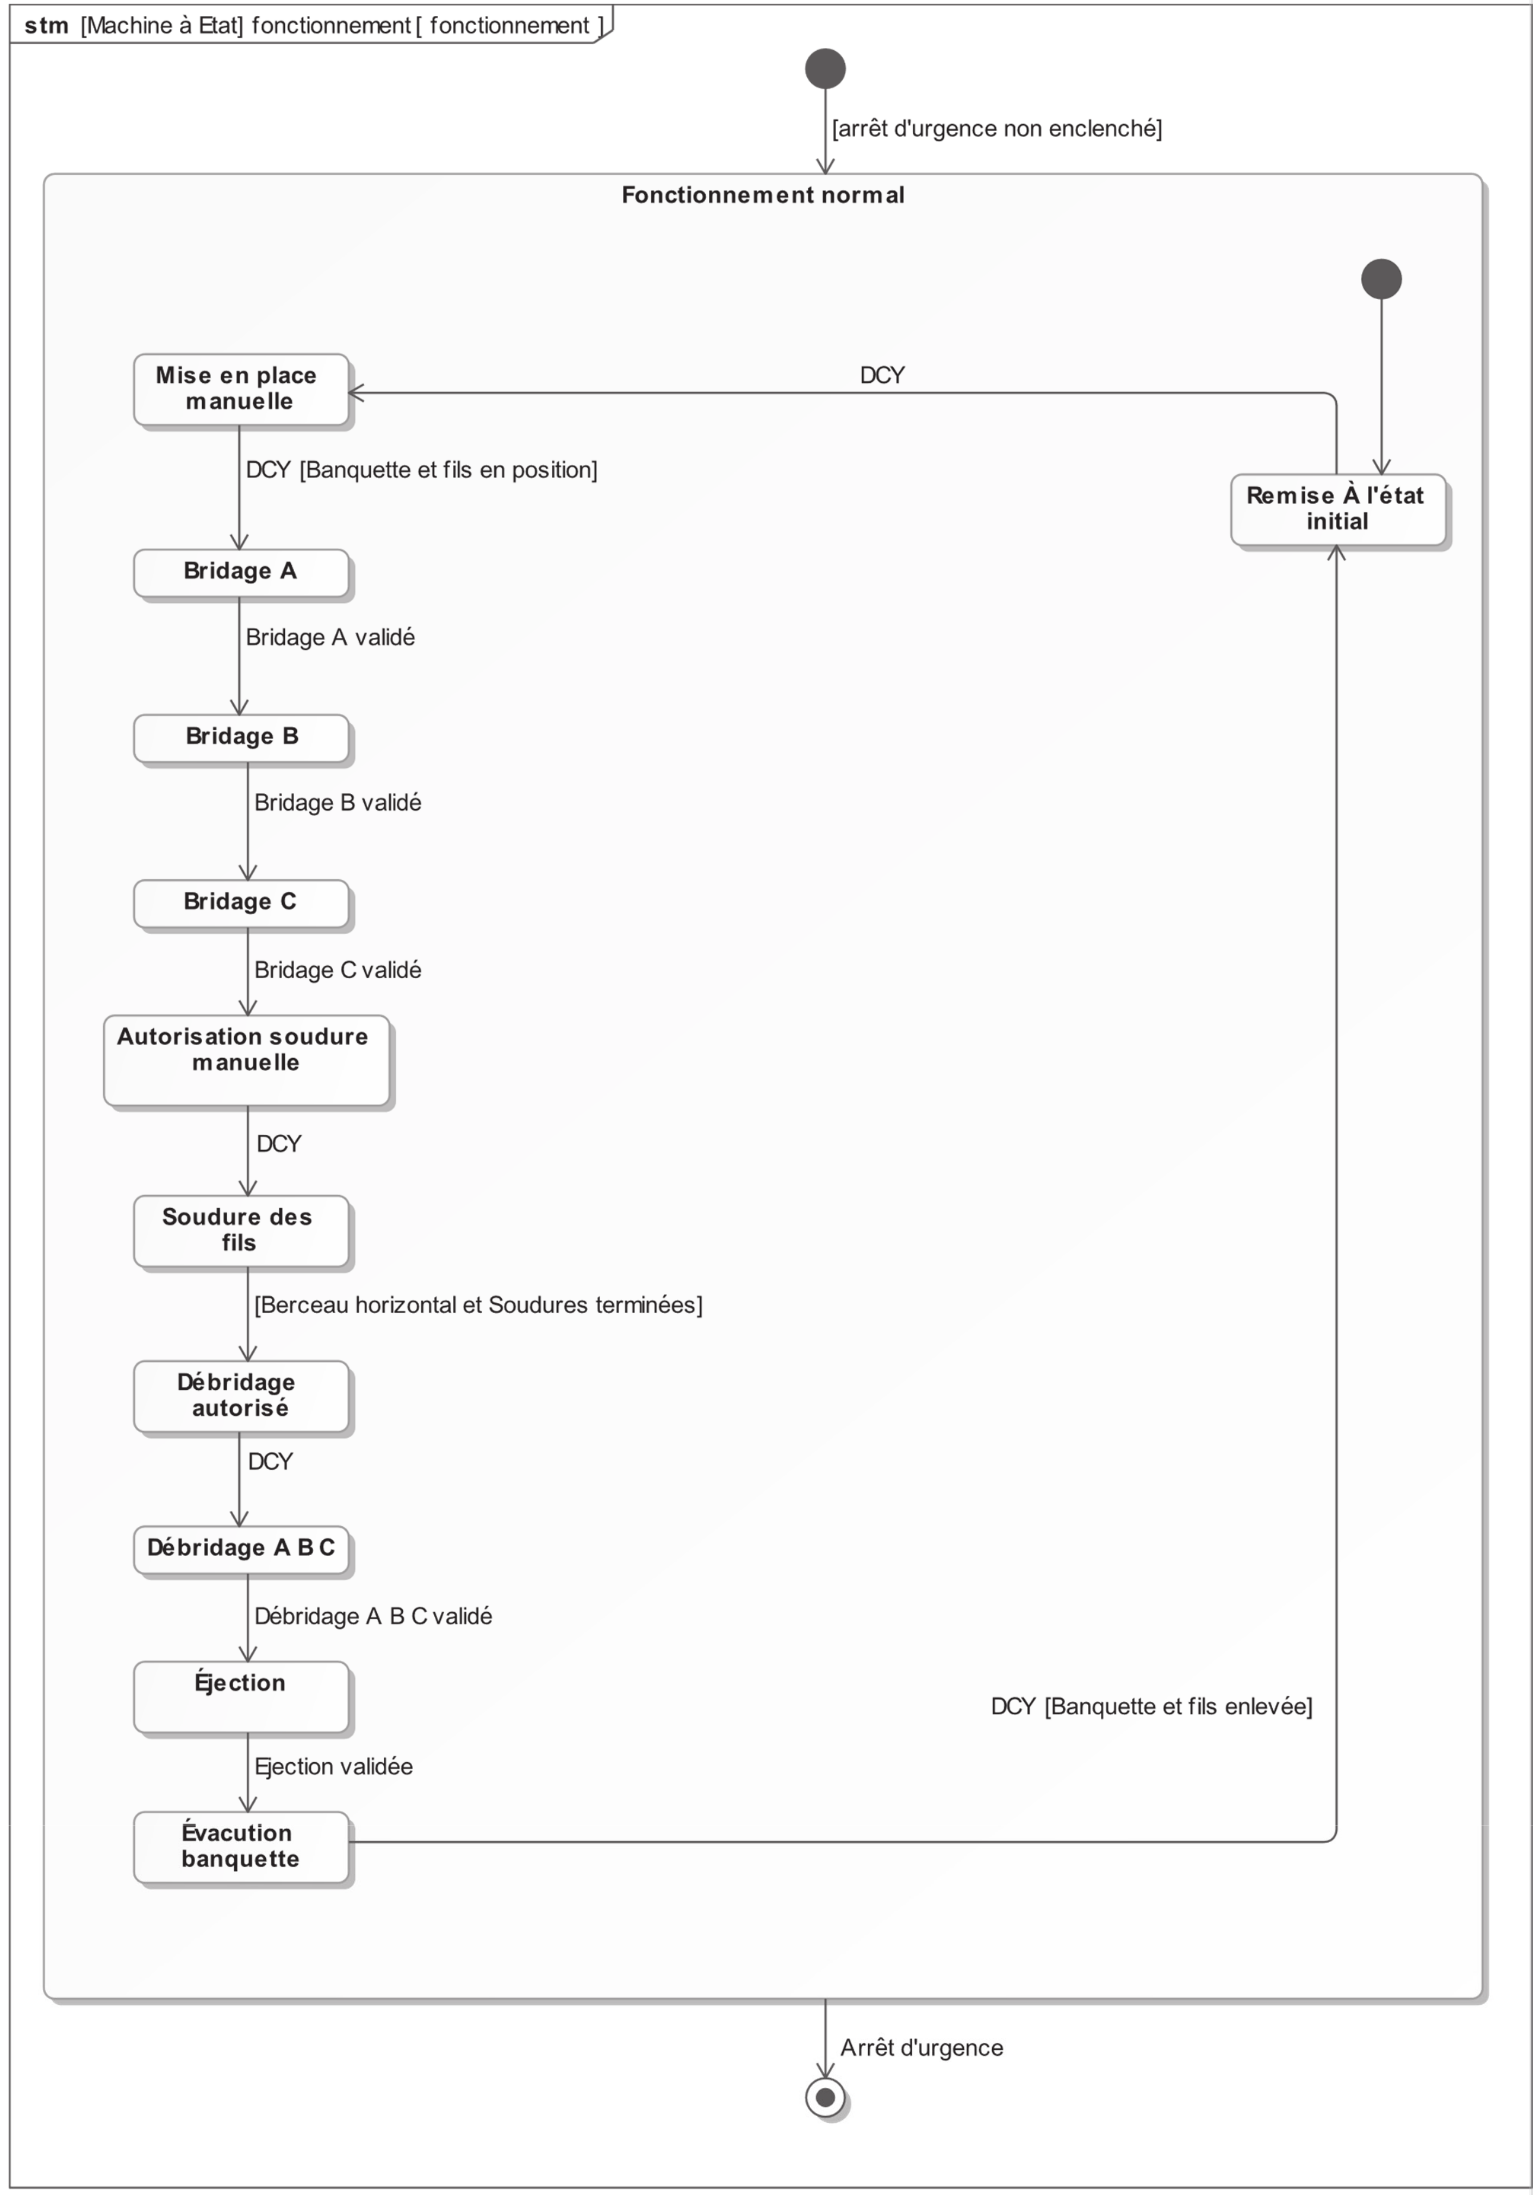
\includegraphics[width=0.8\linewidth]{img/DR04}
\end{center}}{\begin{center}
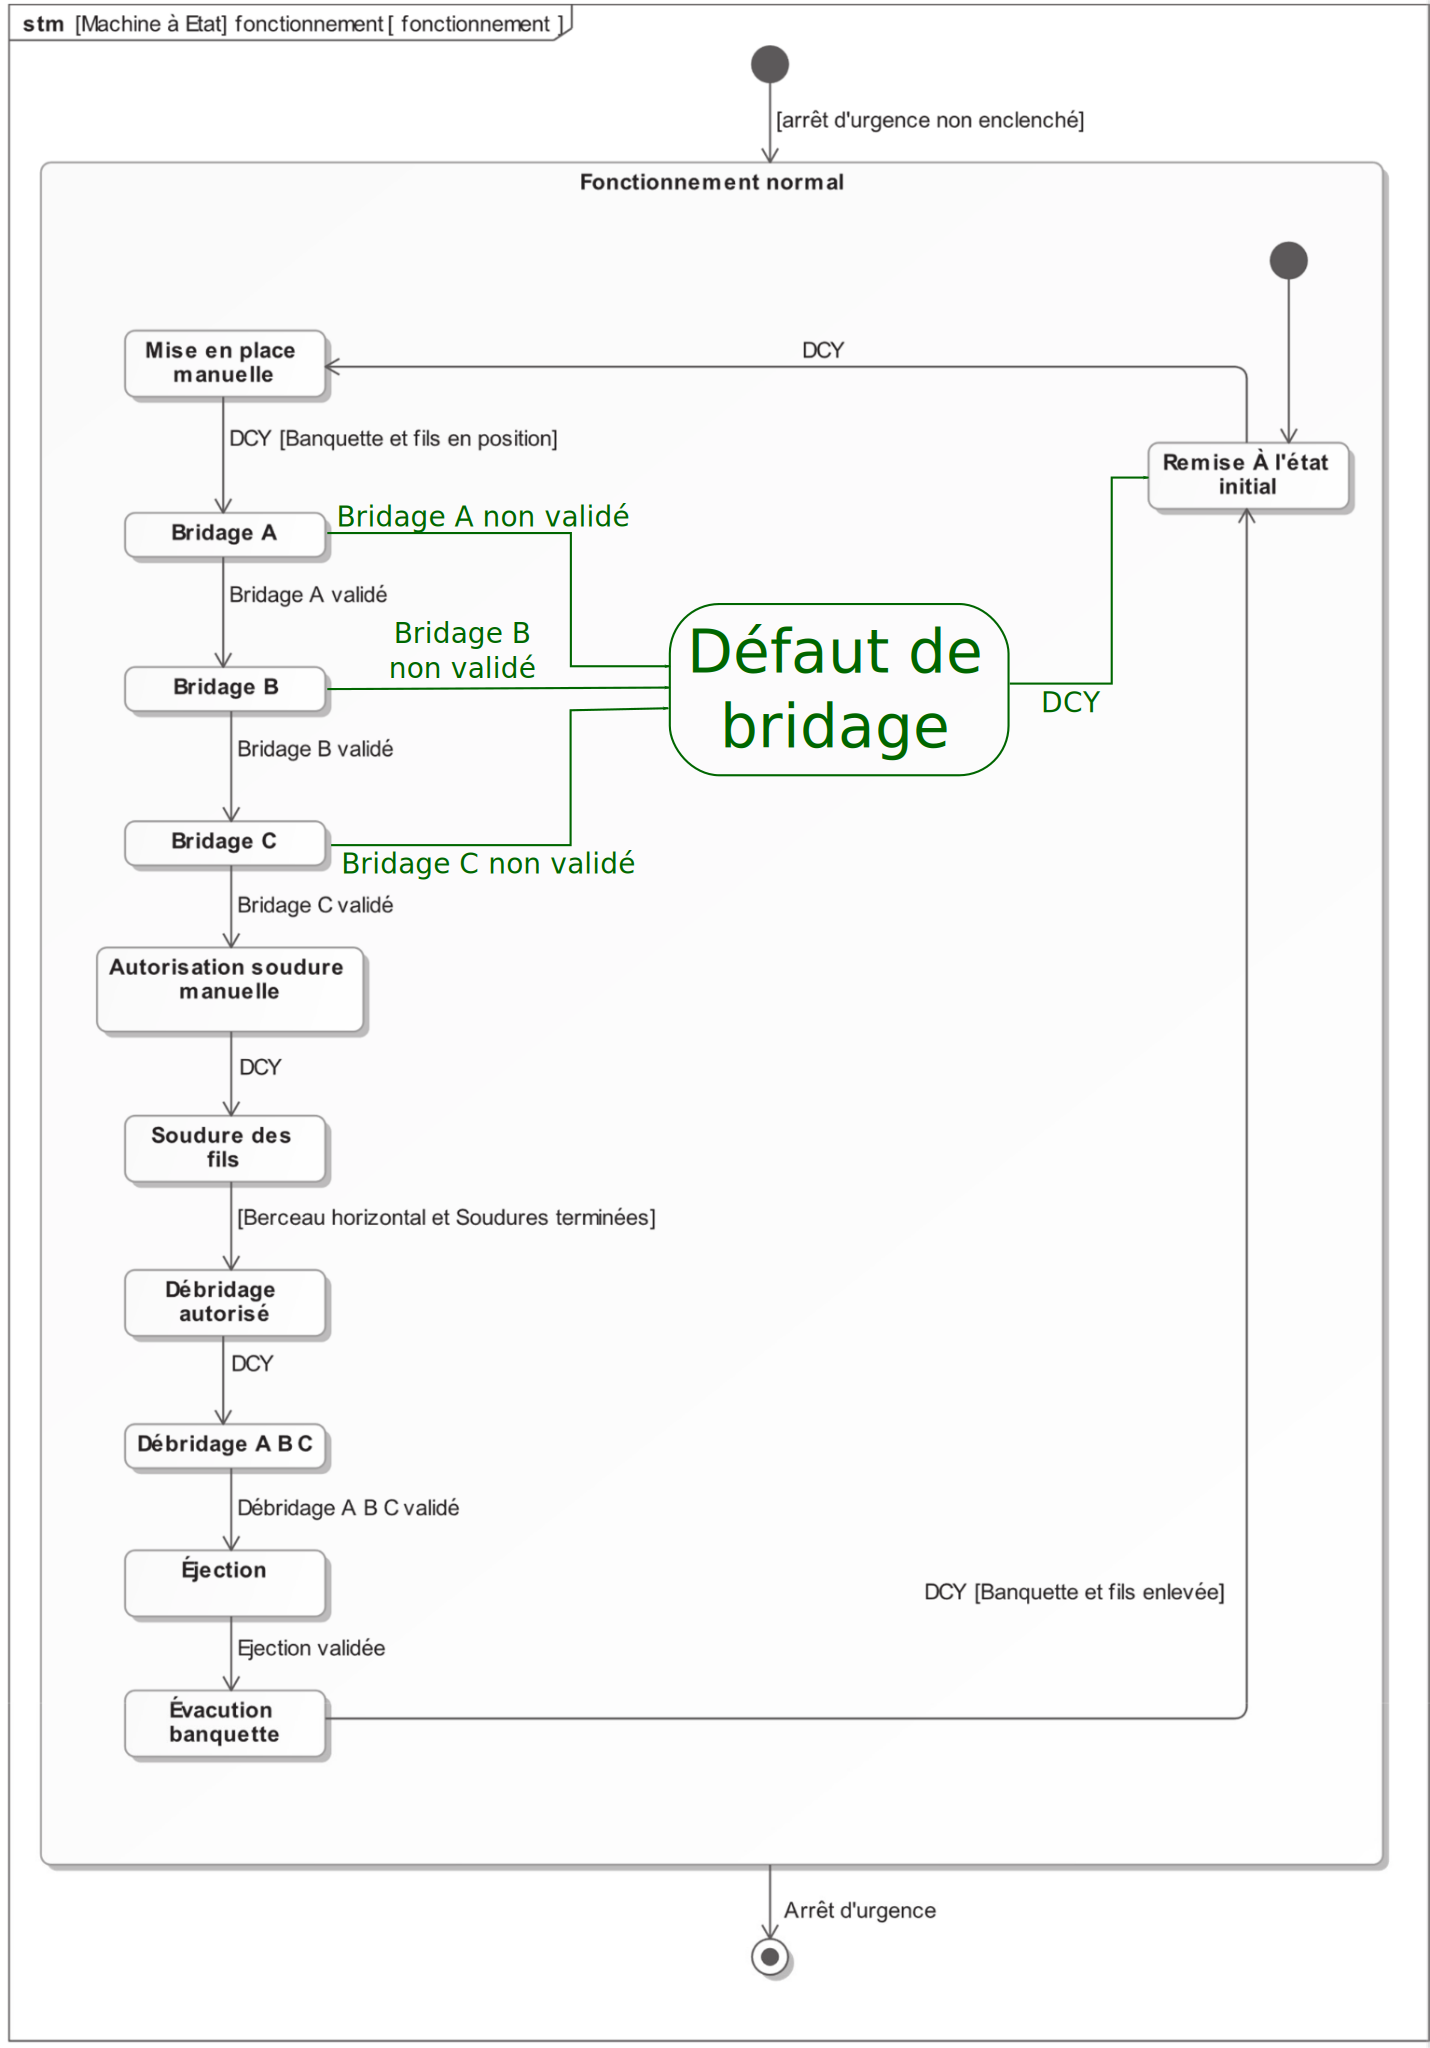
\includegraphics[width=0.8\linewidth]{img/DR04_cor}
\end{center}
}

\reponse{4}{}{
\[\Delta\lambda_{\max}=L\cdot\tan\alpha\]

\[\Delta\lambda_{\max}=1000\cdot\tan 0,1\degree\]

\[\Delta\lambda_{\max}=1000\cdot\tan \frac{0,1\cdot 2\cdot \pi}{6\cdot 60}\]

\[\Delta\lambda_{\max}=1000\cdot\tan \frac{10^{-2}}{6}\]

\[\Delta\lambda_{\max}=1000\cdot\frac{10^{-2}}{6}\]

\[\Delta\lambda_{\max}=1.66mm\]
}

\reponse{5}{}{
\begin{center}
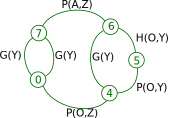
\includegraphics[width=0.8\linewidth]{img/Q18_cor}
\end{center}
}

\reponse{4}{}{
\[h=N_s-r_s\]

\[h=(3\cdot 5+1\cdot 5+3\cdot 5)-(6\cdot(5-1)-1)\]

\[h=35-23=12\]
}

\reponse{4}{}{
\begin{itemize}
 \item supprimer une glissière: $h=7$,
 \item remplacer la glissière entre 4 et 6 par une ponctuelle: $h=3$,
 \item remplacer la pivot en A par une linéaire annulaire : $h=0$.
\end{itemize}
\begin{center}
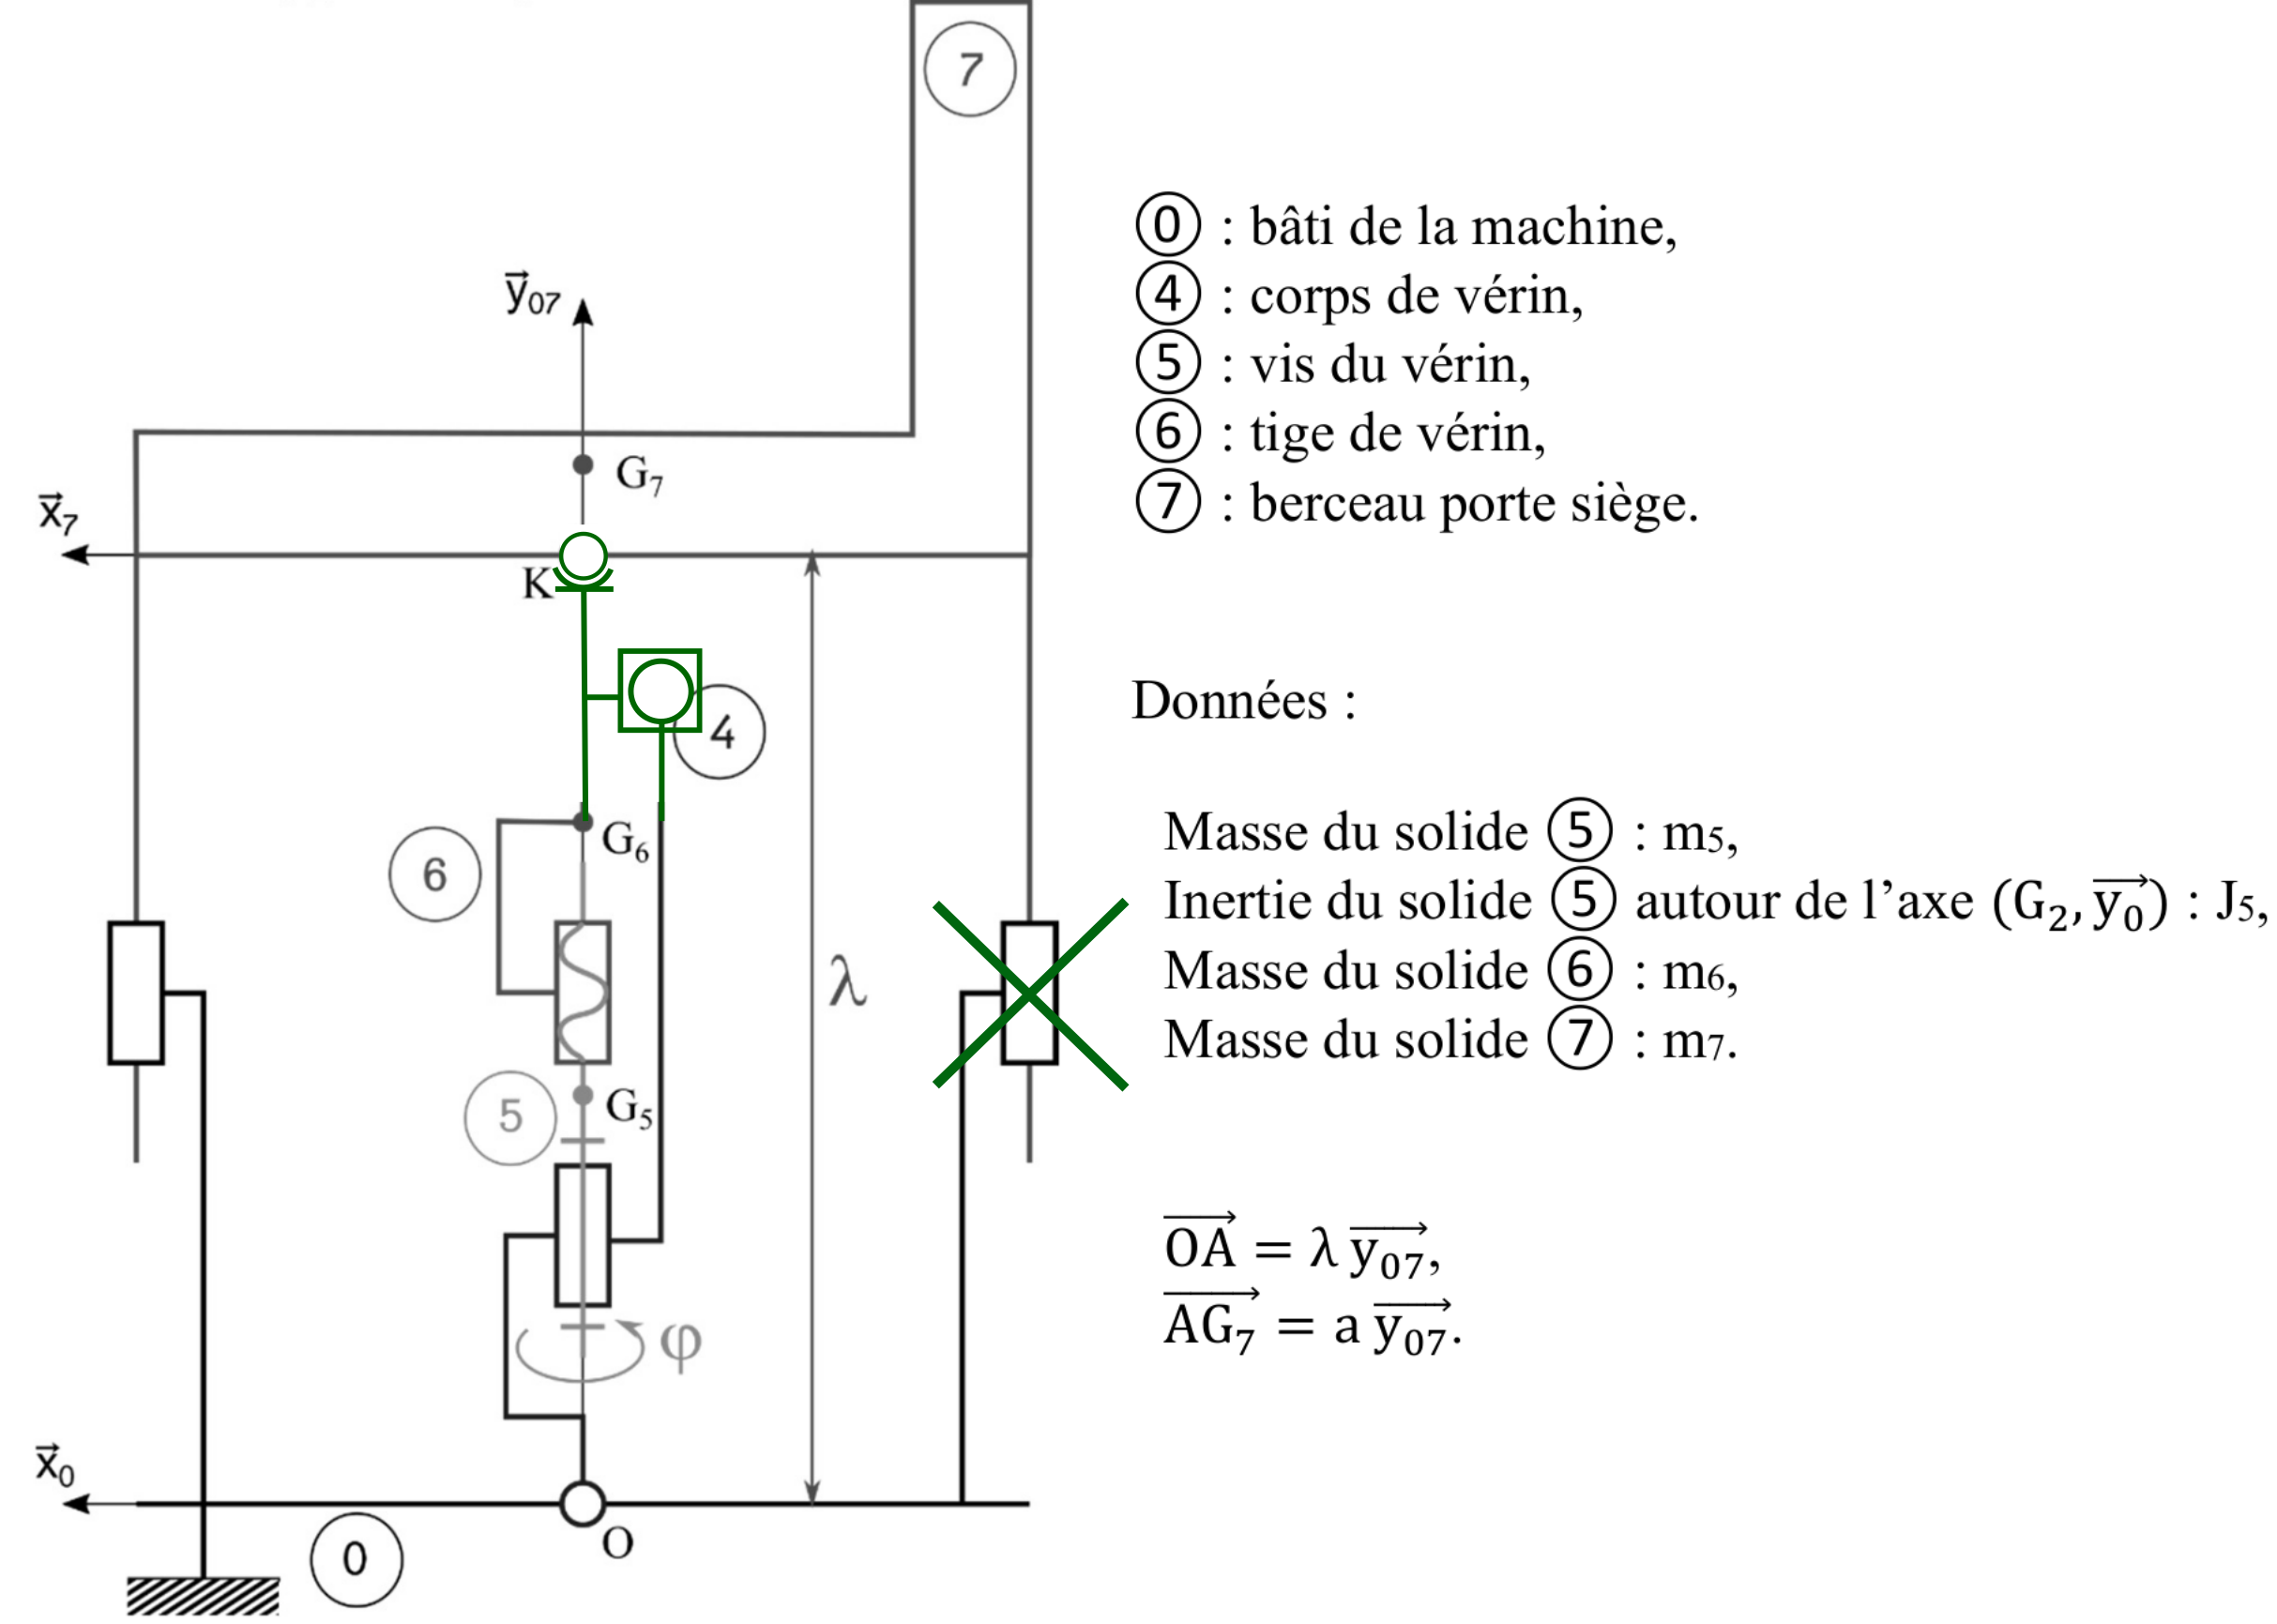
\includegraphics[width=0.8\linewidth]{img/fig20_cor}
\end{center}
}

\reponse{5}{}{
\begin{center}
\begin{circuitikz}
\draw (0,3) to [R, i>^=$i_m(t)$, l=$R$]  (3,3);
\draw (3,3) to [american inductor, l=$L$] (5,3);
\draw (5,3) to [V, l=$e(t)$] (5,0);
\draw (5,0) -- (0,0);
\draw[-triangle 45] (5.5,1.2) -- (5.5,2.0);
\draw[-triangle 45] (-0.2,0) -- (-0.2,3) node[left, midway] {$u_m(p)$};
% utilisation de la librairie arrow
\end{circuitikz} 
\end{center}
}

\reponse{4}{}{
En supposant les conditions nulles:
\[u_{m}(t)\  = R*i_{m}(t)\  + \ L\ \frac{di_{m}(t)}{dt}+\ e(t)\]

\[Um\left( p \right) = \ R*I_{m}\left( p \right) + \ L*p*\ I(p)+\ E\left( p \right)\]
}

\reponse{3}{}{
En supposant les conditions nulles:

\[C_{m}\left( t \right) - C_{mr}\left( t \right) = J_T\frac{d\Omega_{m}(t)}{dt}\]

\[C_{M}\left( p \right) - C_{MR}\left( p \right) = J_T*p{*\Omega}_{M}(p)\]
}

\reponse{3}{}{
\begin{itemize}
 \item $X_1(p)$ est la fem en $V$,
 \item $X_2(p)$ est le couple moteur en $N\cdot M$.
\end{itemize}
}

\reponse{6}{}{
  \[Um\left( p \right) = \ E\left( p \right) + \ R*I\left( p \right) + \ L*p*\ I_{M}(p) \rightarrow Um\left( p \right) - \ E\left( p \right) = \ \left( R + \ L*p \right)\ I_{M}(p)\]

  \[C_{M}\left( p \right) - C_{MR}\left( p \right) = J_T*p{*\Omega}_{M}\left( p \right) + f{*\Omega}_{M}\left( p \right) \rightarrow
C_{M}\left( p \right) - C_{MR}\left( p \right) = J_T*p{*\Omega}_{M}\left( p \right)\]

  \[E\left( p \right) = K*\ \Omega_{M}(p)\]

  \[C_{M}\left( p \right) = K*I_{M}(p)\]

Donc, 
\begin{eqnarray}
H_{1}\left( p \right) = \frac{\frac{1}{R}}{1+\frac{L}{R}p} \nonumber \\ 
H_{2}\left( p \right) = \frac{1}{J_{T}p} \nonumber
\end{eqnarray}
}

\reponse{7}{}{

En prenant $C_m(p)=0$ et $L=0$, on obtient le schéma bloc suivant:
\begin{center}
\begin{tikzpicture}
\sbEntree{E}
\sbComp{comp}{E}
\sbRelier[$U_m(p)$]{E}{comp}
\sbBloc{H1}{$\frac{1}{R}$}{comp}
\sbRelier{comp}{H1}
\sbBloc{K}{$K$}{H1}
\sbRelier{H1}{K}
\sbBloc{sys}{$\frac{1}{J_{T}p}$}{K}
\sbRelier{K}{sys}
\sbSortie{S}{sys}
\sbRelier[$\ \ \ \ \ \ \Omega_m(p)$]{sys}{S}
\sbDecaleNoeudy[4]{S}{U}
\sbDecaleNoeudx[-5]{U}{V}
\sbBlocr{cap}{$K$}{V}
\sbRelieryx{sys-S}{cap}
\sbRelierxy{cap}{comp}
\end{tikzpicture}
\end{center}

\[H\left( p \right) =\frac{\frac{1}{R}\cdot K\cdot \frac{1}{J_T\cdot p}}{1+\frac{1}{R}\cdot K\cdot \frac{1}{J_T\cdot p}\cdot K}=\frac{\frac{K}{R}}{J_T\cdot p+\frac{K^2}{R}}=\frac{\frac{1}{K}}{1 + \frac{RJ_T}{K^2}p} = \frac{K^{'}}{1 + \tau_{m}p}\]

Donc: \[K' = \frac{1}{K}\] et \[\tau_m = \frac{RJ_T}{K^2}\]
}

\reponse{3}{}{
Un codeur incrémental transmet l'angle ou la distance mesuré par une information numérique, suivant différents protocoles. L’information numérique provient d’un système généralement optique comportant une source de lumière, un disque strié et un photodétecteur. Le codeur rotatif permet grâce à un disque (Roue codeuse) comportant des stries de mesurer un déplacement angulaire. Le fait d'avoir deux disques permet de déterminer le sens de rotation.

\begin{center}
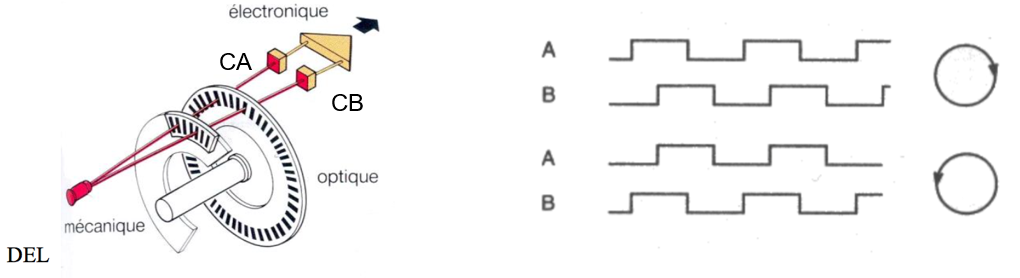
\includegraphics[width=0.8\linewidth]{img/codeur_incremental}
\end{center}
}

\ifdef{\public}{\newpage}

\reponse{5}{}{
Lorsque la tige du vérin se déplace de 1 mm, la vis du vérin,
 effectue un angle \(\Delta\theta_{vis}\), tel que:
 
  \(\Delta\theta_{vis} = \frac{360}{k_{t}} = \frac{360}{12.7} = \frac{3600}{99+27} = \frac{9.400}{9.(11+3)} = \frac{2.200}{2.7} =\frac{210}{7}-\frac{7}{7}-\frac{3}{7}=30-1-0.5= 28.5\degree\).

Le moteur tourne alors d'un angle \(\Delta\theta_{mot}\):
  \(\Delta\theta_{mot} = \frac{\Delta\theta_{vis}}{k_{r}} = 28.5*3.5 =28.5*(3+0.5) = 85.5+14.25=99.75\degree\).

Il faut donc \(360/99.75\approx 3.6\), donc 4 impulsions par tour.
}


\reponse{8}{}{

On trouve \[B'=\frac{B}{k_r\cdot k_t}\]

Donc, on obtient le schéma bloc suivant:
\begin{center}
\begin{tikzpicture}
\sbEntree{E}
\sbComp{comp}{E}
\sbRelier[$Dc(p)\ $]{E}{comp}
\sbBloc{B}{$B'$}{comp}
\sbRelier{comp}{B}
\sbBloc{C}{$C$}{B}
\begin{tiny}
\sbRelier[$\varepsilon(p)$]{B}{C}
\end{tiny}
\sbBloc{A}{$A$}{C}
\begin{tiny}
\sbRelier[$U_c(p)$]{C}{A}
\end{tiny}
\sbBloc{H}{$H(p)$}{A}
\begin{tiny}
\sbRelier[$U_M(p)$]{A}{H}
\end{tiny}
\sbBloc{I}{$\frac{1}{p}$}{H}
\begin{tiny}
\sbRelier[$\Omega_M(p)$]{H}{I}
\end{tiny}
\sbBloc{KR}{$k_r$}{I}
\begin{tiny}
\sbRelier[$\theta_M(p)$]{I}{KR}
\end{tiny}
\sbBloc{KT}{$k_t$}{KR}
\begin{tiny}
\sbRelier[$\theta_R(p)$]{KR}{KT}
\end{tiny}
\sbSortie{S}{KT}
\sbRelier[$\ \ \ \ \ \ D(p)$]{KT}{S}
\sbRenvoi{KT-S}{comp}{}
\end{tikzpicture}
\end{center}
}

\reponse{5}{}{
 \[G(p) = \frac{A\cdot B\cdot K'}{\left( 1 + \tau_{m}p \right)p} = \frac{A_0}{\left( 1 + \tau_{m}p \right)p}\]\\
donc : \[A_0 = A\cdot B\cdot K'\]
}

\ifdef{\public}{\newpage}

\reponse{3}{\begin{center}
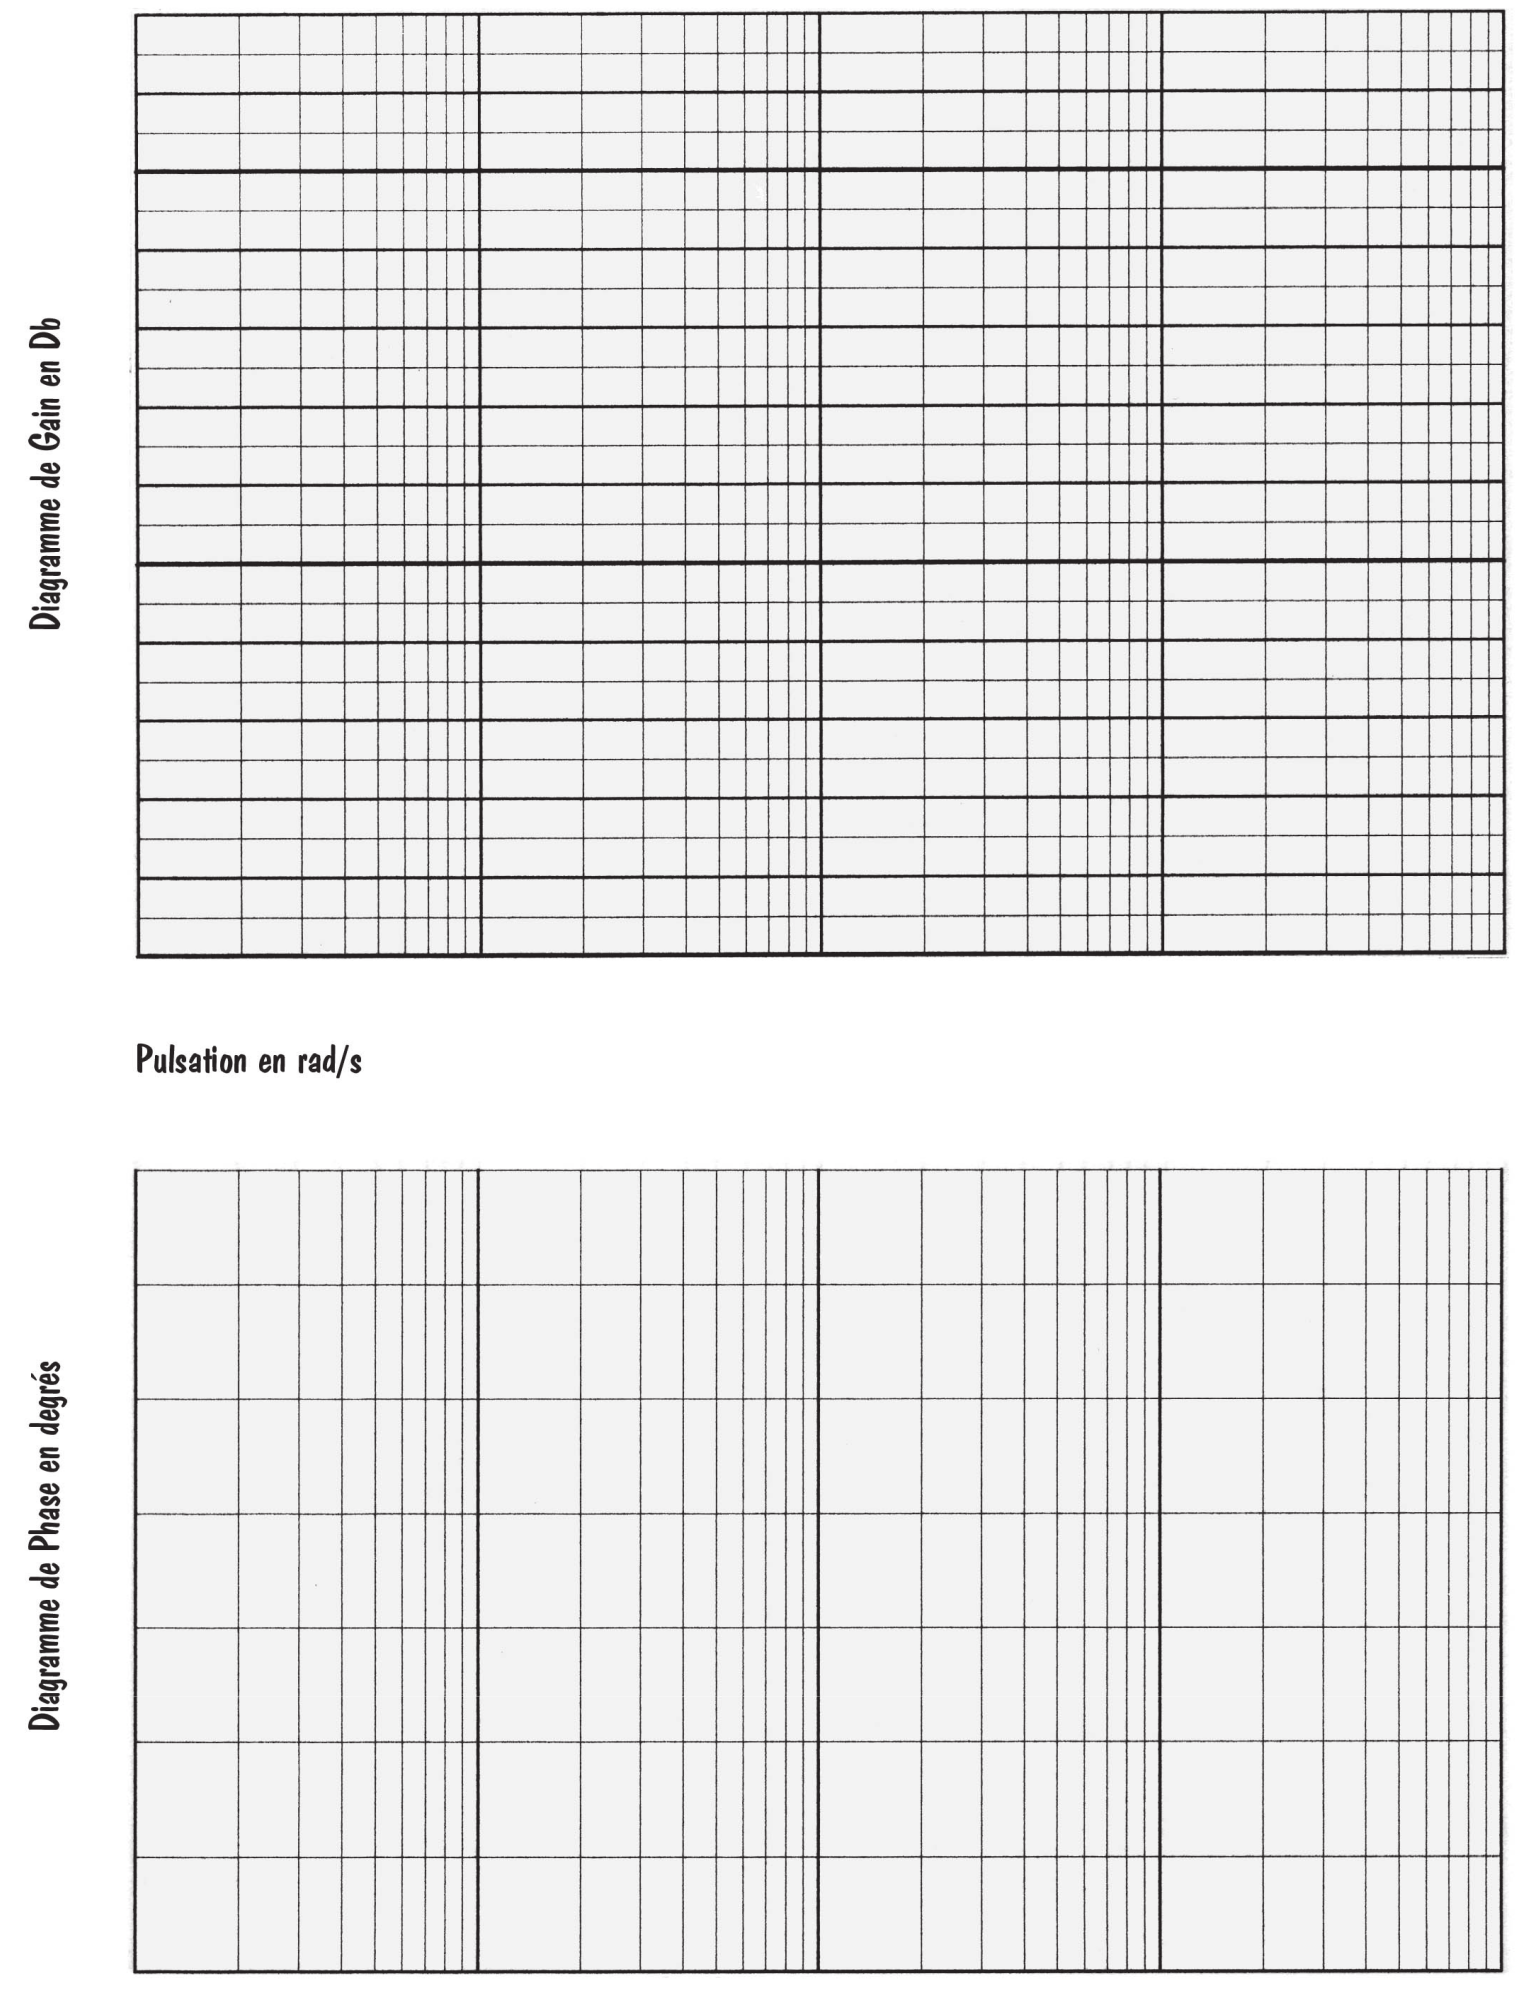
\includegraphics[width=0.8\linewidth]{img/DR05}
\end{center}}{\begin{center}
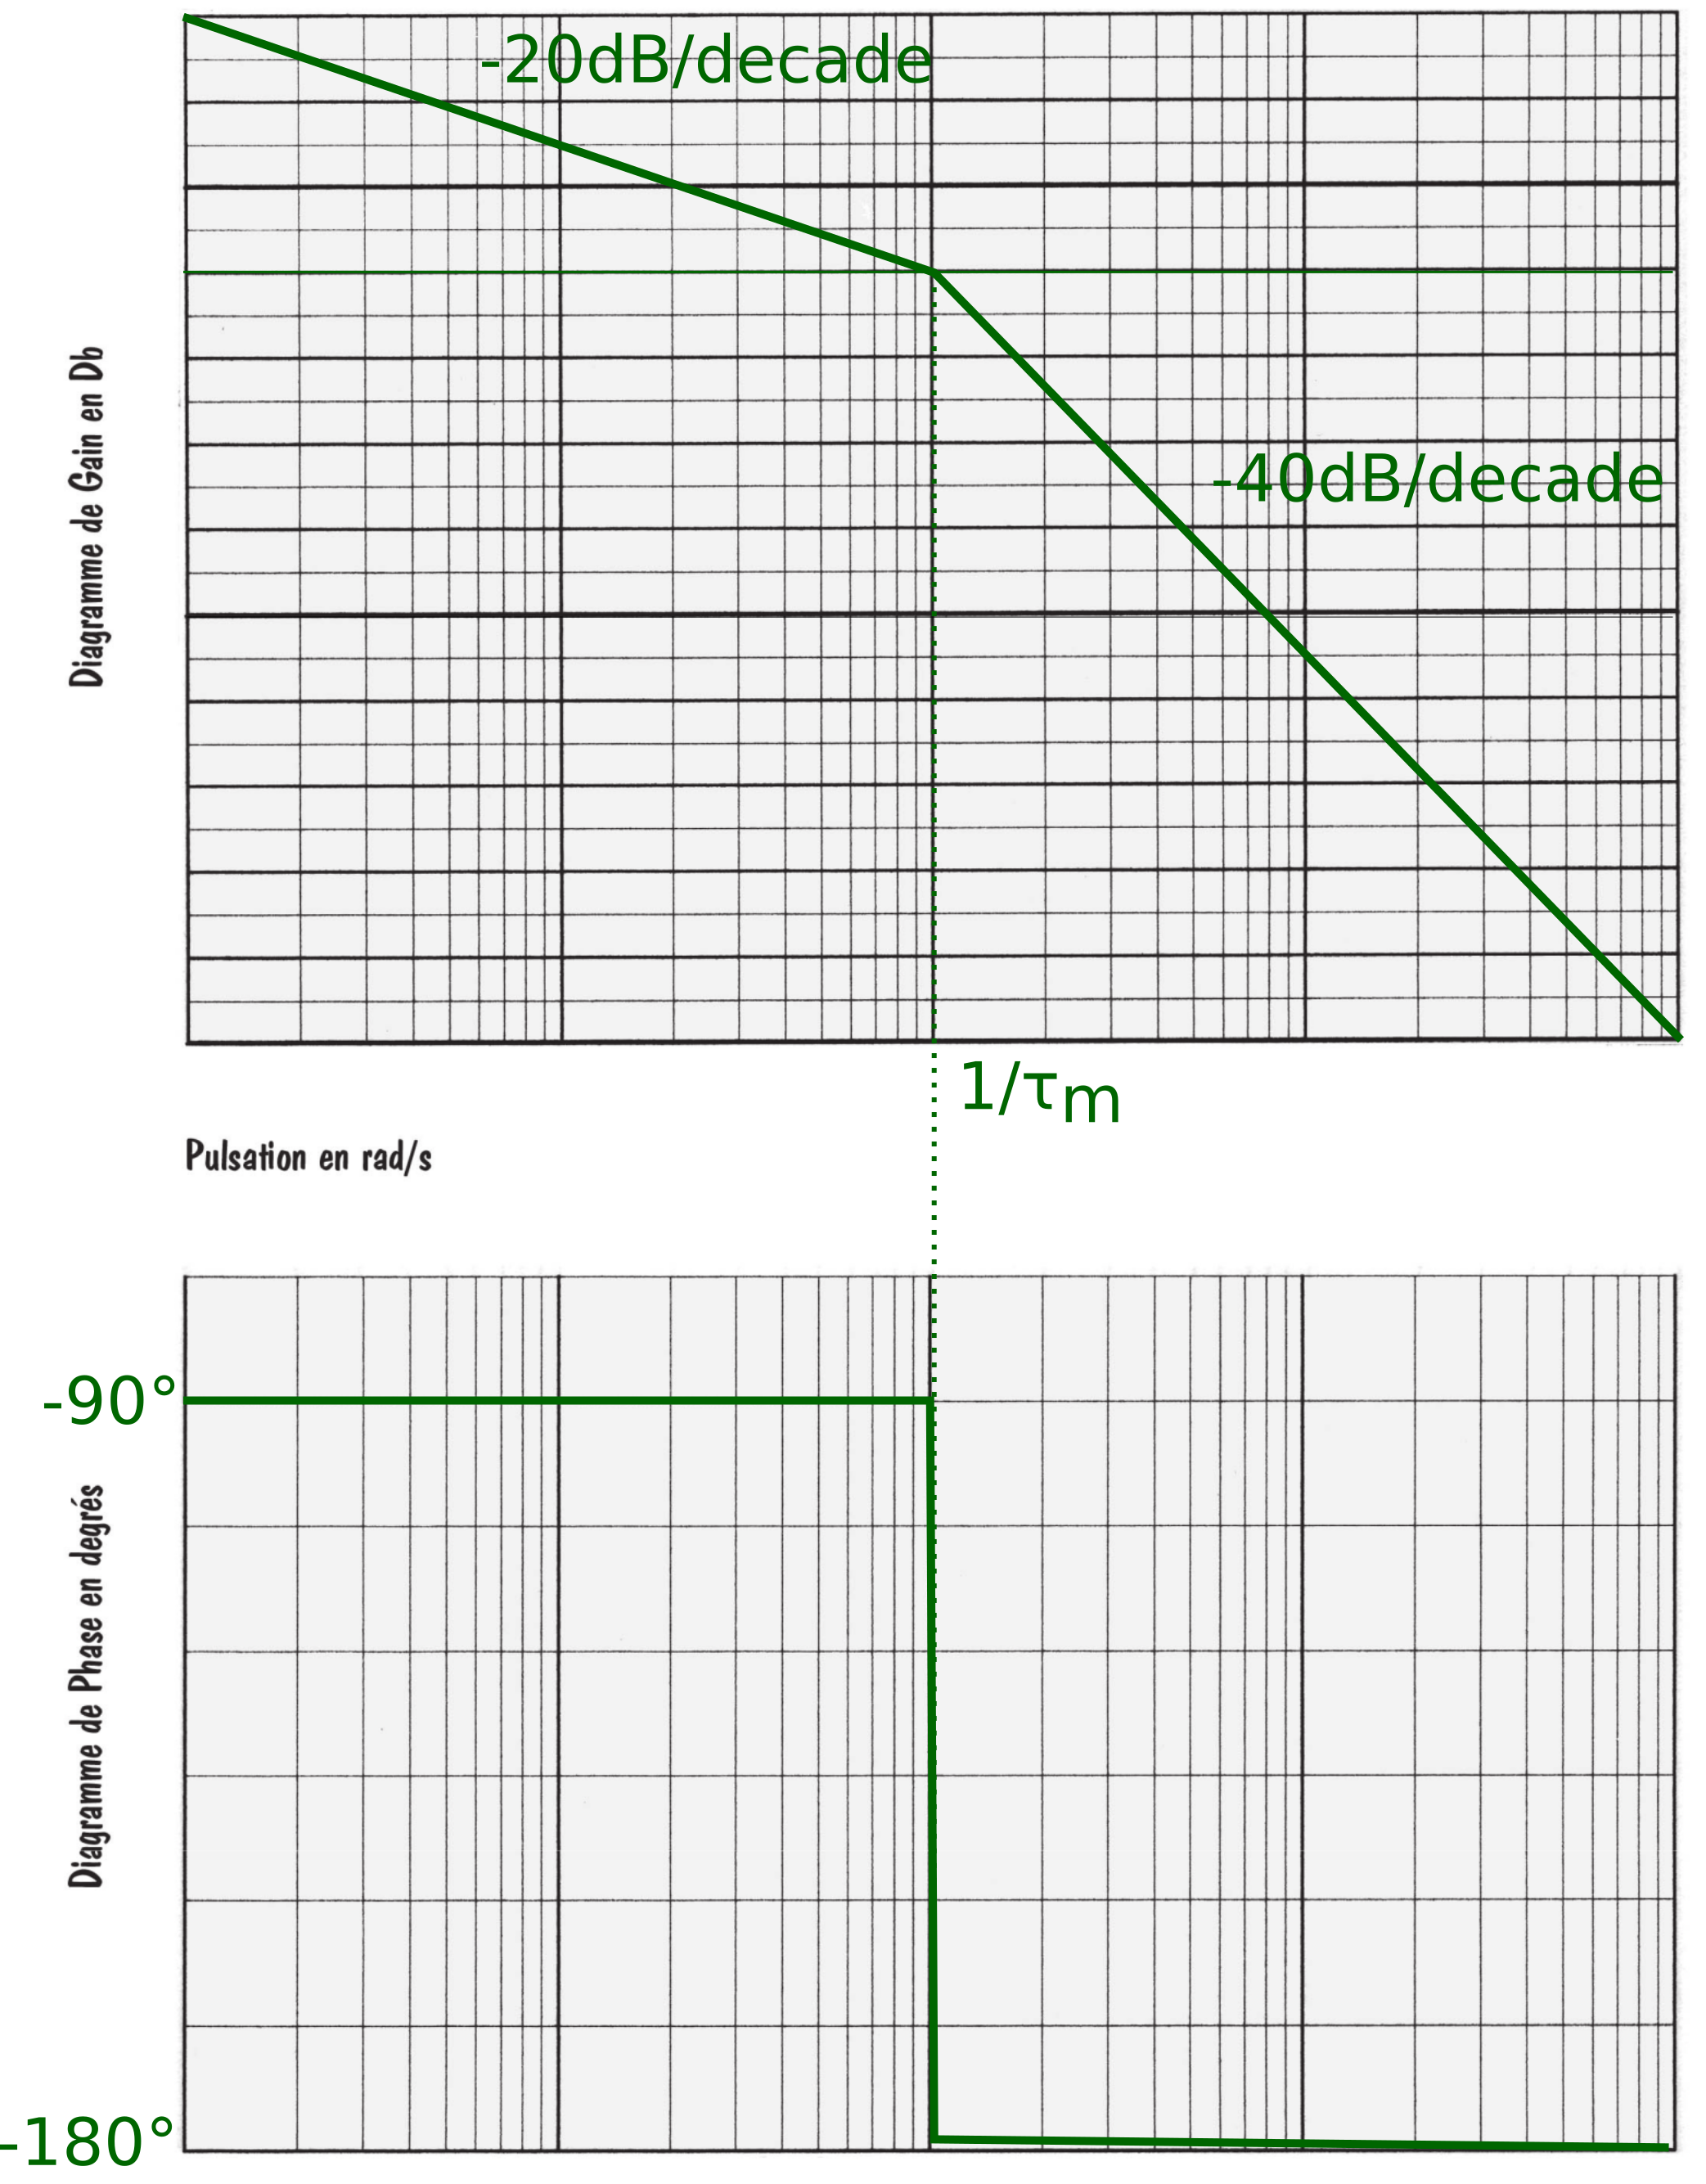
\includegraphics[width=0.8\linewidth]{img/DR05_cor}
\end{center}
}

\ifdef{\public}{\newpage}

\reponse{3}{\begin{center}
\includegraphics[width=0.8\linewidth]{img/DR06}
\end{center}}{\begin{center}
\includegraphics[width=0.8\linewidth]{img/DR06_cor}
\end{center}

\[A_0=\frac{9}{10}\]

\[\tau\approx1.15s\]

\[C\cdot A_0=\sqrt{2}\]

\[C=\frac{\sqrt{2}}{A_0}=\frac{10\cdot \sqrt{2}}{9}\]
}

\ifdef{\public}{\newpage}

\reponse{3}{
\begin{center}
\begin{tikzpicture}
  \draw[->] (-3, 0) -- (3, 0) node[right] {$\Omega_m$};
  \draw[->] (0, -3) -- (0, 3) node[above] {$C_m$};
\node[align=left] at (-0.2,-0.2) {0};
\end{tikzpicture}
\end{center}
}{
Le moteur doit pouvoir fonctionner en moteur dans les deux sens (montée et descente). Et la charge ne peut pas l'entraîner, donc il ne fonctionnera pas en générateur.

\begin{center}
\begin{tikzpicture}
  \draw[->] (-3, 0) -- (3, 0) node[right] {$\Omega_m$};
  \draw[->] (0, -3) -- (0, 3) node[above] {$C_m$};
  \draw[pattern=north west lines, pattern color=blue] (0,0) rectangle (2,-2);
  \draw[pattern=north west lines, pattern color=blue] (0,0) rectangle (-2,2);
\node[align=left] at (-0.2,-0.2) {0};
\node[align=left] at (1.5,1) {$C_m>0$\\$\Omega_m>0$\\ Fonctionnement\\ en moteur};
\node[align=left] at (-1.5,-1) {$C_m<0$\\$\Omega_m<0$\\ Fonctionnement\\ en moteur};
\end{tikzpicture}
\end{center}
}


\reponse{4}{}{
Les interrupteurs non spécifiés dans la suite sont ouverts.

\begin{itemize}
 \item Cas 1: $U_m=E$ si $H_1$ et $H_4$ fermés
 \item Cas 2: $U_m=-E$ si $H_2$ et $H_3$ fermés
 \item Cas 3: $U_m=0$ si $H_1$ et $H_2$ fermés ou exclusif $H_3$ et $H_4$  fermés.
\end{itemize}

Ainsi, pour piloter le moteur avec $U_m>0$ il faut alterner entre:
\begin{itemize}
 \item le cas 1 et le cas 2 avec un rapport cyclique plus grand que 50\%,
 \item le cas 1 et un des cas 3 avec un rapport cyclique plus grand que 0\%. 
\end{itemize}

}


\end{document}